\section{Data and Sample}
\label{empirics}

\subsection{Measuring Spatial Proximity of Conflict to Urban Centers}

Our theoretical framework centers around the argument that variation in macroeconomic growth amongst countries in the midst of civil war can be explained by the spatial proximity between civil conflicts and urban centers. In constructing our dataset, we thus restrict the cases we include to only those country-years in which there was an internal armed conflict. Additionally, the unit of observation for this analysis is the country-year. This enables us to directly explore whether variation in growth amongst countries experiencing internal conflict can be explained by the proximity of conflict to cities.

To measure macroeconomic performance, we focus on annual percent change in GDP from the World Development Indicators. We adopt this parameterization of our dependent variable because we expect that conflicts proximate to urban centers will generate abrupt changes in macroeconomic growth. Much of the extant literature linking internal armed conflict and economic growth has approached this instead using five or ten year averages of GDP growth. However, averaging over an arbitrary set of years may obfuscate meaningful variation in GDP growth over short temporal spans.

We collect information on the location of conflicts from the PRIO Conflict Site Dataset \citep{hallberg:2012}. This dataset contains information on the geographical centers of armed conflict events and the area covered by each conflict at a yearly level from 1989 to 2008. In recent years, other geo-referenced datasets have been developed that go beyond just providing information on conflict centroids and area to providing an actual spatial grid structure through which to conduct analysis (e.g., \citealt{tollefsen:etal:2012}). For the purpose of this analysis, however, we deliberately avoid using these datasets since our primary interest is in examining variation in changes to GDP growth due to the proximity of conflict to urban centers. 

% Note to Ben: Does that sound convincing? Probably not. The point that I'm trying to get across is that using the gridded data is not at the appropriate level of analysis. We need to say something here about this so if you can think of something better that'd be great.

To construct a time-series cross-sectional database of urban centers, we turn to yearly editions of The World Almanac from 1989 to 2008. More refined subnational data listing urban centers by their contribution to economic output would be the most direct way to test our hypothesis, however, cross-national data such as this over the time period of our analysis, especially for developing countries, is simply not available. The World Alamanac lists the major cities in a country by population, thus providing us with a second best approximation of the urban centers that are most relevant for a particular national economy. Typically, the Almanacs list at least three major cities, including the capital, for each country and year from 1989 to 2008. We use the top five major cities listed for each country and then determine their geographical centers.

% Again if you could add anything to why The World Alamanac data is the right choice that would be great.

Using our geo-referenced conflict and urban center data, we proceed to compute the proximity of every civil armed conflict in a country-year from every urban center listed in that year.\footnote{Distances between centroid locations were computed using an iterative method of distance calculation proposed by \citet{vincenty:1975}.} Since our unit of analysis is the country-year, we aggregate the distance between conflicts and major cities by calculating the  minimum logged distance any conflict is from a major city. For example, if a country faces, four conflicts in a year, the datapoint for that country-year level would be the minimum distance any conflict centroid is from any city centroid. This choice of aggregation is what conforms closest to our theoretical claims about macroeconomic activity only being severely disrupted in cases of conflicts being proximate to major cities. 

\begin{figure}
	\centering
	\resizebox{.8\textwidth}{!}{% Created by tikzDevice version 0.8.1 on 2016-01-23 06:21:33
% !TEX encoding = UTF-8 Unicode
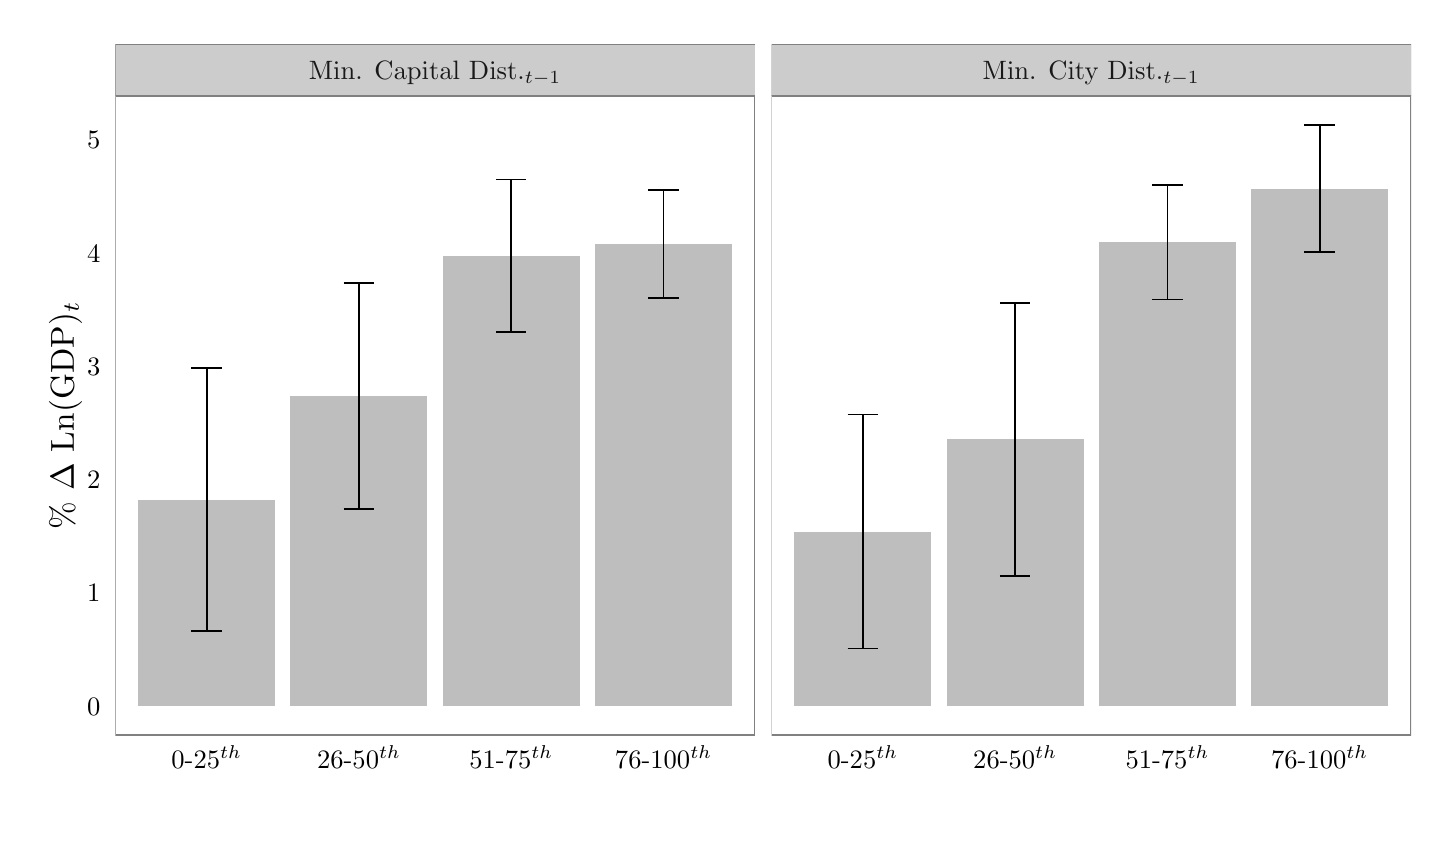
\begin{tikzpicture}[x=1pt,y=1pt]
\definecolor{fillColor}{RGB}{255,255,255}
\path[use as bounding box,fill=fillColor,fill opacity=0.00] (0,0) rectangle (505.89,289.08);
\begin{scope}
\path[clip] (  0.00,  0.00) rectangle (505.89,289.08);
\definecolor{drawColor}{RGB}{255,255,255}
\definecolor{fillColor}{RGB}{255,255,255}

\path[draw=drawColor,line width= 0.6pt,line join=round,line cap=round,fill=fillColor] (  0.00,  0.00) rectangle (505.89,289.08);
\end{scope}
\begin{scope}
\path[clip] ( 31.66, 33.48) rectangle (262.78,264.47);
\definecolor{fillColor}{RGB}{255,255,255}

\path[fill=fillColor] ( 31.66, 33.48) rectangle (262.78,264.47);
\definecolor{fillColor}{RGB}{190,190,190}

\path[fill=fillColor] ( 39.92, 43.98) rectangle ( 89.44,118.52);

\path[fill=fillColor] ( 94.94, 43.98) rectangle (144.47,156.08);

\path[fill=fillColor] (149.97, 43.98) rectangle (199.50,206.62);

\path[fill=fillColor] (205.00, 43.98) rectangle (254.52,210.92);
\definecolor{drawColor}{RGB}{0,0,0}

\path[draw=drawColor,line width= 0.6pt,line join=round] ( 59.18,166.05) --
	( 70.18,166.05);

\path[draw=drawColor,line width= 0.6pt,line join=round] ( 64.68,166.05) --
	( 64.68, 70.99);

\path[draw=drawColor,line width= 0.6pt,line join=round] ( 59.18, 70.99) --
	( 70.18, 70.99);

\path[draw=drawColor,line width= 0.6pt,line join=round] (114.20,196.90) --
	(125.21,196.90);

\path[draw=drawColor,line width= 0.6pt,line join=round] (119.71,196.90) --
	(119.71,115.25);

\path[draw=drawColor,line width= 0.6pt,line join=round] (114.20,115.25) --
	(125.21,115.25);

\path[draw=drawColor,line width= 0.6pt,line join=round] (169.23,234.20) --
	(180.24,234.20);

\path[draw=drawColor,line width= 0.6pt,line join=round] (174.73,234.20) --
	(174.73,179.04);

\path[draw=drawColor,line width= 0.6pt,line join=round] (169.23,179.04) --
	(180.24,179.04);

\path[draw=drawColor,line width= 0.6pt,line join=round] (224.26,230.50) --
	(235.26,230.50);

\path[draw=drawColor,line width= 0.6pt,line join=round] (229.76,230.50) --
	(229.76,191.33);

\path[draw=drawColor,line width= 0.6pt,line join=round] (224.26,191.33) --
	(235.26,191.33);
\definecolor{drawColor}{gray}{0.50}

\path[draw=drawColor,line width= 0.6pt,line join=round,line cap=round] ( 31.66, 33.48) rectangle (262.78,264.47);
\end{scope}
\begin{scope}
\path[clip] (268.78, 33.48) rectangle (499.89,264.47);
\definecolor{fillColor}{RGB}{255,255,255}

\path[fill=fillColor] (268.78, 33.48) rectangle (499.89,264.47);
\definecolor{fillColor}{RGB}{190,190,190}

\path[fill=fillColor] (277.03, 43.98) rectangle (326.56,107.02);

\path[fill=fillColor] (332.06, 43.98) rectangle (381.58,140.28);

\path[fill=fillColor] (387.08, 43.98) rectangle (436.61,211.59);

\path[fill=fillColor] (442.11, 43.98) rectangle (491.64,230.95);
\definecolor{drawColor}{RGB}{0,0,0}

\path[draw=drawColor,line width= 0.6pt,line join=round] (296.29,149.26) --
	(307.30,149.26);

\path[draw=drawColor,line width= 0.6pt,line join=round] (301.79,149.26) --
	(301.79, 64.78);

\path[draw=drawColor,line width= 0.6pt,line join=round] (296.29, 64.78) --
	(307.30, 64.78);

\path[draw=drawColor,line width= 0.6pt,line join=round] (351.32,189.55) --
	(362.32,189.55);

\path[draw=drawColor,line width= 0.6pt,line join=round] (356.82,189.55) --
	(356.82, 91.00);

\path[draw=drawColor,line width= 0.6pt,line join=round] (351.32, 91.00) --
	(362.32, 91.00);

\path[draw=drawColor,line width= 0.6pt,line join=round] (406.34,232.29) --
	(417.35,232.29);

\path[draw=drawColor,line width= 0.6pt,line join=round] (411.85,232.29) --
	(411.85,190.89);

\path[draw=drawColor,line width= 0.6pt,line join=round] (406.34,190.89) --
	(417.35,190.89);

\path[draw=drawColor,line width= 0.6pt,line join=round] (461.37,253.97) --
	(472.38,253.97);

\path[draw=drawColor,line width= 0.6pt,line join=round] (466.87,253.97) --
	(466.87,207.94);

\path[draw=drawColor,line width= 0.6pt,line join=round] (461.37,207.94) --
	(472.38,207.94);
\definecolor{drawColor}{gray}{0.50}

\path[draw=drawColor,line width= 0.6pt,line join=round,line cap=round] (268.78, 33.48) rectangle (499.89,264.47);
\end{scope}
\begin{scope}
\path[clip] ( 31.66,264.47) rectangle (262.78,283.08);
\definecolor{drawColor}{gray}{0.50}
\definecolor{fillColor}{gray}{0.80}

\path[draw=drawColor,line width= 0.2pt,line join=round,line cap=round,fill=fillColor] ( 31.66,264.47) rectangle (262.78,283.08);
\definecolor{drawColor}{gray}{0.10}

\node[text=drawColor,anchor=base,inner sep=0pt, outer sep=0pt, scale=  0.96] at (147.22,270.47) {Min. Capital Dist.$_{t-1}$};
\end{scope}
\begin{scope}
\path[clip] (268.78,264.47) rectangle (499.89,283.08);
\definecolor{drawColor}{gray}{0.50}
\definecolor{fillColor}{gray}{0.80}

\path[draw=drawColor,line width= 0.2pt,line join=round,line cap=round,fill=fillColor] (268.78,264.47) rectangle (499.89,283.08);
\definecolor{drawColor}{gray}{0.10}

\node[text=drawColor,anchor=base,inner sep=0pt, outer sep=0pt, scale=  0.96] at (384.33,270.47) {Min. City Dist.$_{t-1}$};
\end{scope}
\begin{scope}
\path[clip] (  0.00,  0.00) rectangle (505.89,289.08);
\definecolor{drawColor}{RGB}{0,0,0}

\node[text=drawColor,anchor=base east,inner sep=0pt, outer sep=0pt, scale=  0.96] at ( 26.26, 40.67) {0};

\node[text=drawColor,anchor=base east,inner sep=0pt, outer sep=0pt, scale=  0.96] at ( 26.26, 81.59) {1};

\node[text=drawColor,anchor=base east,inner sep=0pt, outer sep=0pt, scale=  0.96] at ( 26.26,122.51) {2};

\node[text=drawColor,anchor=base east,inner sep=0pt, outer sep=0pt, scale=  0.96] at ( 26.26,163.44) {3};

\node[text=drawColor,anchor=base east,inner sep=0pt, outer sep=0pt, scale=  0.96] at ( 26.26,204.36) {4};

\node[text=drawColor,anchor=base east,inner sep=0pt, outer sep=0pt, scale=  0.96] at ( 26.26,245.28) {5};
\end{scope}
\begin{scope}
\path[clip] (  0.00,  0.00) rectangle (505.89,289.08);
\definecolor{drawColor}{RGB}{0,0,0}

\node[text=drawColor,anchor=base,inner sep=0pt, outer sep=0pt, scale=  0.96] at ( 64.68, 21.46) {0-25$^{th}$};

\node[text=drawColor,anchor=base,inner sep=0pt, outer sep=0pt, scale=  0.96] at (119.71, 21.46) {26-50$^{th}$};

\node[text=drawColor,anchor=base,inner sep=0pt, outer sep=0pt, scale=  0.96] at (174.73, 21.46) {51-75$^{th}$};

\node[text=drawColor,anchor=base,inner sep=0pt, outer sep=0pt, scale=  0.96] at (229.76, 21.46) {76-100$^{th}$};
\end{scope}
\begin{scope}
\path[clip] (  0.00,  0.00) rectangle (505.89,289.08);
\definecolor{drawColor}{RGB}{0,0,0}

\node[text=drawColor,anchor=base,inner sep=0pt, outer sep=0pt, scale=  0.96] at (301.79, 21.46) {0-25$^{th}$};

\node[text=drawColor,anchor=base,inner sep=0pt, outer sep=0pt, scale=  0.96] at (356.82, 21.46) {26-50$^{th}$};

\node[text=drawColor,anchor=base,inner sep=0pt, outer sep=0pt, scale=  0.96] at (411.85, 21.46) {51-75$^{th}$};

\node[text=drawColor,anchor=base,inner sep=0pt, outer sep=0pt, scale=  0.96] at (466.87, 21.46) {76-100$^{th}$};
\end{scope}
\begin{scope}
\path[clip] (  0.00,  0.00) rectangle (505.89,289.08);
\definecolor{drawColor}{RGB}{0,0,0}

\node[text=drawColor,rotate= 90.00,anchor=base,inner sep=0pt, outer sep=0pt, scale=  1.20] at ( 16.66,148.97) {\% $\Delta$ Ln(GDP)$_{t}$};
\end{scope}
\end{tikzpicture}
}
	\caption{Average relationship between city and capital distance from conflict and GDP growth.}
	\label{fig:distGdp}
\end{figure}

In figure \ref{fig:CityConfMap}, we show the geographic distribution of conflicts and cities. The centroid locations of conflicts are shown by red dots. Not surprisingly, we can see that in many cases conflict locations are clustered within specific parts of a country. In most cases, this clustering is indicative of the same conflict moving within the geographic boundaries of a country over time. The blue diamonds in \ref{fig:CityConfMap} denote the locations of major cities as identified in The World Alamanacs from 1989 to 2008. Countries shaded in grey are those for which no armed conflict took place in this period according to the PRIO dataset.  

\begin{amssidewaysfigure}
	\centering
	\includegraphics[width=1\textwidth]{CityConfMap-crop}
	\caption{This map illustrates the geographic distribution of all conflicts, according to the PRIO Conflict Site Dataset, and major cities listed in The World Almanac from 1989 to 2008. Countries for which no armed conflicts are recorded are shaded in grey.}
	\label{fig:CityConfMap}
\end{amssidewaysfigure}
\FloatBarrier

\subsection{Control Variables}

From the PRIO dataset we also bring in additional information about that conflict, specifically its intensity, the area of conflict, whether the conflict involves a territorial dispute, and its duration.

Last, we include a number of additional control measures. First, we control for a country's total, logged land area to differentiate between the proximity effects of conflicts within large and small countries. We also control for a couple of macroeconomic variables that could affect year over year changes in GDP, specifically, lagged inflation and whether or not the state is an upper income country, as defined by the World Bank.

Add in descriptors for each of these variables and expectations of their sign.

A drawback with circular conflict zones is that they cover more territory than is actually affected by the conflict, including territories of neighboring countries.4 Due to the nature of armed conflict it may be impossible to gain information on the exact locations of armed encounters, occupied territories, and rebel bases. It might be possible to map the actual conflict-affected area with high precision for some well- reported conflicts, but it would be virtually impossible to code all conflict-years in the dataset coherently in a similar manner. The operationalization of conflict zones is essentially a trade-off between precision and simplicity, and in most cases a circular conflict zone will give a good indication of the core area of the conflict.

Using a dataset that includes 497 country-years of civil war from 68 different countries during the period of 1989 to 2007. 

To estimate the model we use random effects clustered on countries. The model we estimate is shown below:

\begin{align*}
	\% \Delta Log(GDP_{i,t}) &= \beta_{1}(Ln(Min. \; Conflict \; Dist.)_{i,t}) \\
	& \;+\; \beta_{2}(Conflict \; Intensity_{i,t}) \;+\; \beta_{3}(Conflict \; Type_{i,t}) \\
	& \;+\; \beta_{4}(Conflict \; Duration_{i,t}) \;+\; \beta_{5}(Ln(Conflict \; Area)_{i,t}) \\	
	& \;+\; \beta_{6}(Upper \; Income_{i,t}) \;+\; \beta_{7}(Inflation_{i,t-1}) \\
	&  \;+\; \beta_{8}(Democracy_{i,t-1}) \;+\; \beta_{9}(Resource \; Rents/GDP_{t}) \\
	& \;+\; \beta_{10}(World \; GDP \; Growth_{t}) \;+\; \mu_{i,t} \;+\; \epsilon_{i,t}
\end{align*}

\section{Results}
\label{findings} 

We depict the results of our model in figure \ref{fig:coefPlot}. Most of the findings here are in line with our theoretical expectations. We find that higher levels of conflict intensity are associated with lower levels of GDP growth. The effect of conflict type is positive, indicating that non-territorial disputes are related to lower levels of GDP growth as well. Surprisingly, conflicts that are of a longer duration are, on average, not having a negative effect on GDP growth. 

Most importantly, we find strong support for our key hypothesis relating the proximity of a conflict to lower levels of GDP growth. The fact that the logged, minimum conflict distance variable is positive indicates that conflicts closer to major cities have an adverse effect on economic growth. 

\begin{figure}
	\centering
	\begin{tabular}{cc}
		\subfloat[SubFigure 1][Capital City]{
			\resizebox{.45\textwidth}{!}{% Created by tikzDevice version 0.7.0 on 2014-09-23 11:36:12
% !TEX encoding = UTF-8 Unicode
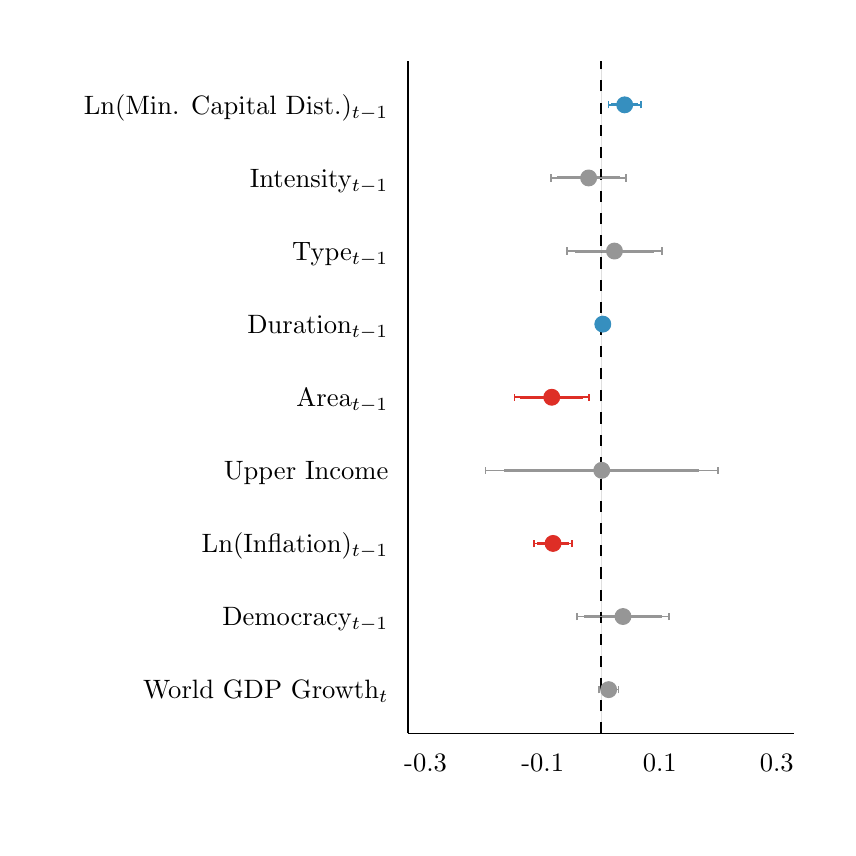
\begin{tikzpicture}[x=1pt,y=1pt]
\definecolor[named]{fillColor}{rgb}{1.00,1.00,1.00}
\path[use as bounding box,fill=fillColor,fill opacity=0.00] (0,0) rectangle (289.08,289.08);
\begin{scope}
\path[clip] (  0.00,  0.00) rectangle (289.08,289.08);
\definecolor[named]{drawColor}{rgb}{1.00,1.00,1.00}
\definecolor[named]{fillColor}{rgb}{1.00,1.00,1.00}

\path[draw=drawColor,line width= 0.6pt,line join=round,line cap=round,fill=fillColor] ( -0.00,  0.00) rectangle (289.08,289.08);
\end{scope}
\begin{scope}
\path[clip] (137.46, 34.03) rectangle (277.03,277.03);
\definecolor[named]{fillColor}{rgb}{1.00,1.00,1.00}

\path[fill=fillColor] (137.46, 34.03) rectangle (277.03,277.03);
\definecolor[named]{drawColor}{rgb}{0.59,0.59,0.59}
\definecolor[named]{fillColor}{rgb}{0.59,0.59,0.59}

\path[draw=drawColor,draw opacity=0.30,line width= 0.3pt,line join=round,fill=fillColor,fill opacity=0.30] (206.43, 49.88) -- (213.45, 49.88);

\path[draw=drawColor,draw opacity=0.30,line width= 0.3pt,line join=round,fill=fillColor,fill opacity=0.30] (198.47, 76.30) -- (231.75, 76.30);
\definecolor[named]{drawColor}{rgb}{0.87,0.18,0.15}
\definecolor[named]{fillColor}{rgb}{0.87,0.18,0.15}

\path[draw=drawColor,draw opacity=0.30,line width= 0.3pt,line join=round,fill=fillColor,fill opacity=0.30] (183.03,102.71) -- (196.68,102.71);
\definecolor[named]{drawColor}{rgb}{0.59,0.59,0.59}
\definecolor[named]{fillColor}{rgb}{0.59,0.59,0.59}

\path[draw=drawColor,draw opacity=0.30,line width= 0.3pt,line join=round,fill=fillColor,fill opacity=0.30] (165.42,129.12) -- (249.46,129.12);
\definecolor[named]{drawColor}{rgb}{0.87,0.18,0.15}
\definecolor[named]{fillColor}{rgb}{0.87,0.18,0.15}

\path[draw=drawColor,draw opacity=0.30,line width= 0.3pt,line join=round,fill=fillColor,fill opacity=0.30] (175.86,155.53) -- (202.88,155.53);
\definecolor[named]{drawColor}{rgb}{0.21,0.56,0.75}
\definecolor[named]{fillColor}{rgb}{0.21,0.56,0.75}

\path[draw=drawColor,draw opacity=0.30,line width= 0.3pt,line join=round,fill=fillColor,fill opacity=0.30] (207.28,181.95) -- (208.37,181.95);
\definecolor[named]{drawColor}{rgb}{0.59,0.59,0.59}
\definecolor[named]{fillColor}{rgb}{0.59,0.59,0.59}

\path[draw=drawColor,draw opacity=0.30,line width= 0.3pt,line join=round,fill=fillColor,fill opacity=0.30] (194.89,208.36) -- (229.18,208.36);

\path[draw=drawColor,draw opacity=0.30,line width= 0.3pt,line join=round,fill=fillColor,fill opacity=0.30] (189.15,234.77) -- (216.25,234.77);
\definecolor[named]{drawColor}{rgb}{0.21,0.56,0.75}
\definecolor[named]{fillColor}{rgb}{0.21,0.56,0.75}

\path[draw=drawColor,draw opacity=0.30,line width= 0.3pt,line join=round,fill=fillColor,fill opacity=0.30] (209.85,261.19) -- (221.60,261.19);
\definecolor[named]{drawColor}{rgb}{0.59,0.59,0.59}
\definecolor[named]{fillColor}{rgb}{0.59,0.59,0.59}

\path[draw=drawColor,line width= 1.1pt,line join=round,fill=fillColor] (206.99, 49.88) -- (212.88, 49.88);

\path[draw=drawColor,line width= 1.1pt,line join=round,fill=fillColor] (201.15, 76.30) -- (229.08, 76.30);
\definecolor[named]{drawColor}{rgb}{0.87,0.18,0.15}
\definecolor[named]{fillColor}{rgb}{0.87,0.18,0.15}

\path[draw=drawColor,line width= 1.1pt,line join=round,fill=fillColor] (184.13,102.71) -- (195.58,102.71);
\definecolor[named]{drawColor}{rgb}{0.59,0.59,0.59}
\definecolor[named]{fillColor}{rgb}{0.59,0.59,0.59}

\path[draw=drawColor,line width= 1.1pt,line join=round,fill=fillColor] (172.18,129.12) -- (242.71,129.12);
\definecolor[named]{drawColor}{rgb}{0.87,0.18,0.15}
\definecolor[named]{fillColor}{rgb}{0.87,0.18,0.15}

\path[draw=drawColor,line width= 1.1pt,line join=round,fill=fillColor] (178.04,155.53) -- (200.70,155.53);
\definecolor[named]{drawColor}{rgb}{0.21,0.56,0.75}
\definecolor[named]{fillColor}{rgb}{0.21,0.56,0.75}

\path[draw=drawColor,line width= 1.1pt,line join=round,fill=fillColor] (207.37,181.95) -- (208.28,181.95);
\definecolor[named]{drawColor}{rgb}{0.59,0.59,0.59}
\definecolor[named]{fillColor}{rgb}{0.59,0.59,0.59}

\path[draw=drawColor,line width= 1.1pt,line join=round,fill=fillColor] (197.65,208.36) -- (226.42,208.36);

\path[draw=drawColor,line width= 1.1pt,line join=round,fill=fillColor] (191.33,234.77) -- (214.07,234.77);
\definecolor[named]{drawColor}{rgb}{0.21,0.56,0.75}
\definecolor[named]{fillColor}{rgb}{0.21,0.56,0.75}

\path[draw=drawColor,line width= 1.1pt,line join=round,fill=fillColor] (210.79,261.19) -- (220.66,261.19);
\definecolor[named]{drawColor}{rgb}{0.00,0.00,0.00}
\definecolor[named]{fillColor}{rgb}{0.00,0.00,0.00}

\path[draw=drawColor,line width= 0.6pt,dash pattern=on 4pt off 4pt ,line join=round,fill=fillColor] (207.25, 34.03) -- (207.25,277.03);
\definecolor[named]{drawColor}{rgb}{0.21,0.56,0.75}
\definecolor[named]{fillColor}{rgb}{0.21,0.56,0.75}

\path[draw=drawColor,line width= 0.4pt,line join=round,line cap=round,fill=fillColor] (215.73,261.19) circle (  2.85);
\definecolor[named]{drawColor}{rgb}{0.59,0.59,0.59}
\definecolor[named]{fillColor}{rgb}{0.59,0.59,0.59}

\path[draw=drawColor,line width= 0.4pt,line join=round,line cap=round,fill=fillColor] (202.70,234.77) circle (  2.85);

\path[draw=drawColor,line width= 0.4pt,line join=round,line cap=round,fill=fillColor] (212.04,208.36) circle (  2.85);
\definecolor[named]{drawColor}{rgb}{0.21,0.56,0.75}
\definecolor[named]{fillColor}{rgb}{0.21,0.56,0.75}

\path[draw=drawColor,line width= 0.4pt,line join=round,line cap=round,fill=fillColor] (207.82,181.95) circle (  2.85);
\definecolor[named]{drawColor}{rgb}{0.87,0.18,0.15}
\definecolor[named]{fillColor}{rgb}{0.87,0.18,0.15}

\path[draw=drawColor,line width= 0.4pt,line join=round,line cap=round,fill=fillColor] (189.37,155.53) circle (  2.85);
\definecolor[named]{drawColor}{rgb}{0.59,0.59,0.59}
\definecolor[named]{fillColor}{rgb}{0.59,0.59,0.59}

\path[draw=drawColor,line width= 0.4pt,line join=round,line cap=round,fill=fillColor] (207.44,129.12) circle (  2.85);
\definecolor[named]{drawColor}{rgb}{0.87,0.18,0.15}
\definecolor[named]{fillColor}{rgb}{0.87,0.18,0.15}

\path[draw=drawColor,line width= 0.4pt,line join=round,line cap=round,fill=fillColor] (189.85,102.71) circle (  2.85);
\definecolor[named]{drawColor}{rgb}{0.59,0.59,0.59}
\definecolor[named]{fillColor}{rgb}{0.59,0.59,0.59}

\path[draw=drawColor,line width= 0.4pt,line join=round,line cap=round,fill=fillColor] (215.11, 76.30) circle (  2.85);

\path[draw=drawColor,line width= 0.4pt,line join=round,line cap=round,fill=fillColor] (209.94, 49.88) circle (  2.85);

\path[draw=drawColor,line width= 0.6pt,line join=round] (213.45, 48.56) --
	(213.45, 51.20);

\path[draw=drawColor,line width= 0.6pt,line join=round] (213.45, 49.88) --
	(206.43, 49.88);

\path[draw=drawColor,line width= 0.6pt,line join=round] (206.43, 48.56) --
	(206.43, 51.20);

\path[draw=drawColor,line width= 0.6pt,line join=round] (231.75, 74.97) --
	(231.75, 77.62);

\path[draw=drawColor,line width= 0.6pt,line join=round] (231.75, 76.30) --
	(198.47, 76.30);

\path[draw=drawColor,line width= 0.6pt,line join=round] (198.47, 74.97) --
	(198.47, 77.62);
\definecolor[named]{drawColor}{rgb}{0.87,0.18,0.15}

\path[draw=drawColor,line width= 0.6pt,line join=round] (196.68,101.39) --
	(196.68,104.03);

\path[draw=drawColor,line width= 0.6pt,line join=round] (196.68,102.71) --
	(183.03,102.71);

\path[draw=drawColor,line width= 0.6pt,line join=round] (183.03,101.39) --
	(183.03,104.03);
\definecolor[named]{drawColor}{rgb}{0.59,0.59,0.59}

\path[draw=drawColor,line width= 0.6pt,line join=round] (249.46,127.80) --
	(249.46,130.44);

\path[draw=drawColor,line width= 0.6pt,line join=round] (249.46,129.12) --
	(165.42,129.12);

\path[draw=drawColor,line width= 0.6pt,line join=round] (165.42,127.80) --
	(165.42,130.44);
\definecolor[named]{drawColor}{rgb}{0.87,0.18,0.15}

\path[draw=drawColor,line width= 0.6pt,line join=round] (202.88,154.21) --
	(202.88,156.86);

\path[draw=drawColor,line width= 0.6pt,line join=round] (202.88,155.53) --
	(175.86,155.53);

\path[draw=drawColor,line width= 0.6pt,line join=round] (175.86,154.21) --
	(175.86,156.86);
\definecolor[named]{drawColor}{rgb}{0.21,0.56,0.75}

\path[draw=drawColor,line width= 0.6pt,line join=round] (208.37,180.63) --
	(208.37,183.27);

\path[draw=drawColor,line width= 0.6pt,line join=round] (208.37,181.95) --
	(207.28,181.95);

\path[draw=drawColor,line width= 0.6pt,line join=round] (207.28,180.63) --
	(207.28,183.27);
\definecolor[named]{drawColor}{rgb}{0.59,0.59,0.59}

\path[draw=drawColor,line width= 0.6pt,line join=round] (229.18,207.04) --
	(229.18,209.68);

\path[draw=drawColor,line width= 0.6pt,line join=round] (229.18,208.36) --
	(194.89,208.36);

\path[draw=drawColor,line width= 0.6pt,line join=round] (194.89,207.04) --
	(194.89,209.68);

\path[draw=drawColor,line width= 0.6pt,line join=round] (216.25,233.45) --
	(216.25,236.09);

\path[draw=drawColor,line width= 0.6pt,line join=round] (216.25,234.77) --
	(189.15,234.77);

\path[draw=drawColor,line width= 0.6pt,line join=round] (189.15,233.45) --
	(189.15,236.09);
\definecolor[named]{drawColor}{rgb}{0.21,0.56,0.75}

\path[draw=drawColor,line width= 0.6pt,line join=round] (221.60,259.87) --
	(221.60,262.51);

\path[draw=drawColor,line width= 0.6pt,line join=round] (221.60,261.19) --
	(209.85,261.19);

\path[draw=drawColor,line width= 0.6pt,line join=round] (209.85,259.87) --
	(209.85,262.51);
\end{scope}
\begin{scope}
\path[clip] (  0.00,  0.00) rectangle (289.08,289.08);
\definecolor[named]{drawColor}{rgb}{0.00,0.00,0.00}

\path[draw=drawColor,line width= 0.6pt,line join=round] (137.46, 34.03) --
	(137.46,277.03);
\end{scope}
\begin{scope}
\path[clip] (  0.00,  0.00) rectangle (289.08,289.08);
\definecolor[named]{drawColor}{rgb}{0.00,0.00,0.00}

\node[text=drawColor,anchor=base east,inner sep=0pt, outer sep=0pt, scale=  0.96] at (130.35, 46.58) {World GDP Growth$_{t}$};

\node[text=drawColor,anchor=base east,inner sep=0pt, outer sep=0pt, scale=  0.96] at (130.35, 72.99) {Democracy$_{t-1}$};

\node[text=drawColor,anchor=base east,inner sep=0pt, outer sep=0pt, scale=  0.96] at (130.35, 99.40) {Ln(Inflation)$_{t-1}$};

\node[text=drawColor,anchor=base east,inner sep=0pt, outer sep=0pt, scale=  0.96] at (130.35,125.82) {Upper Income};

\node[text=drawColor,anchor=base east,inner sep=0pt, outer sep=0pt, scale=  0.96] at (130.35,152.23) {Area$_{t-1}$};

\node[text=drawColor,anchor=base east,inner sep=0pt, outer sep=0pt, scale=  0.96] at (130.35,178.64) {Duration$_{t-1}$};

\node[text=drawColor,anchor=base east,inner sep=0pt, outer sep=0pt, scale=  0.96] at (130.35,205.06) {Type$_{t-1}$};

\node[text=drawColor,anchor=base east,inner sep=0pt, outer sep=0pt, scale=  0.96] at (130.35,231.47) {Intensity$_{t-1}$};

\node[text=drawColor,anchor=base east,inner sep=0pt, outer sep=0pt, scale=  0.96] at (130.35,257.88) {Ln(Min. Capital Dist.)$_{t-1}$};
\end{scope}
\begin{scope}
\path[clip] (  0.00,  0.00) rectangle (289.08,289.08);
\definecolor[named]{drawColor}{rgb}{0.00,0.00,0.00}

\path[draw=drawColor,line width= 0.6pt,line join=round] (137.46, 34.03) --
	(277.03, 34.03);
\end{scope}
\begin{scope}
\path[clip] (  0.00,  0.00) rectangle (289.08,289.08);
\definecolor[named]{drawColor}{rgb}{0.00,0.00,0.00}

\node[text=drawColor,anchor=base,inner sep=0pt, outer sep=0pt, scale=  0.96] at (143.80, 20.31) {-0.3};

\node[text=drawColor,anchor=base,inner sep=0pt, outer sep=0pt, scale=  0.96] at (186.10, 20.31) {-0.1};

\node[text=drawColor,anchor=base,inner sep=0pt, outer sep=0pt, scale=  0.96] at (228.40, 20.31) {0.1};

\node[text=drawColor,anchor=base,inner sep=0pt, outer sep=0pt, scale=  0.96] at (270.69, 20.31) {0.3};
\end{scope}
\end{tikzpicture}
}
		\label{fig:capCoef}} &
		\subfloat[SubFigure 2][Any City]{
			\resizebox{.45\textwidth}{!}{% Created by tikzDevice version 0.7.0 on 2014-09-23 11:36:07
% !TEX encoding = UTF-8 Unicode
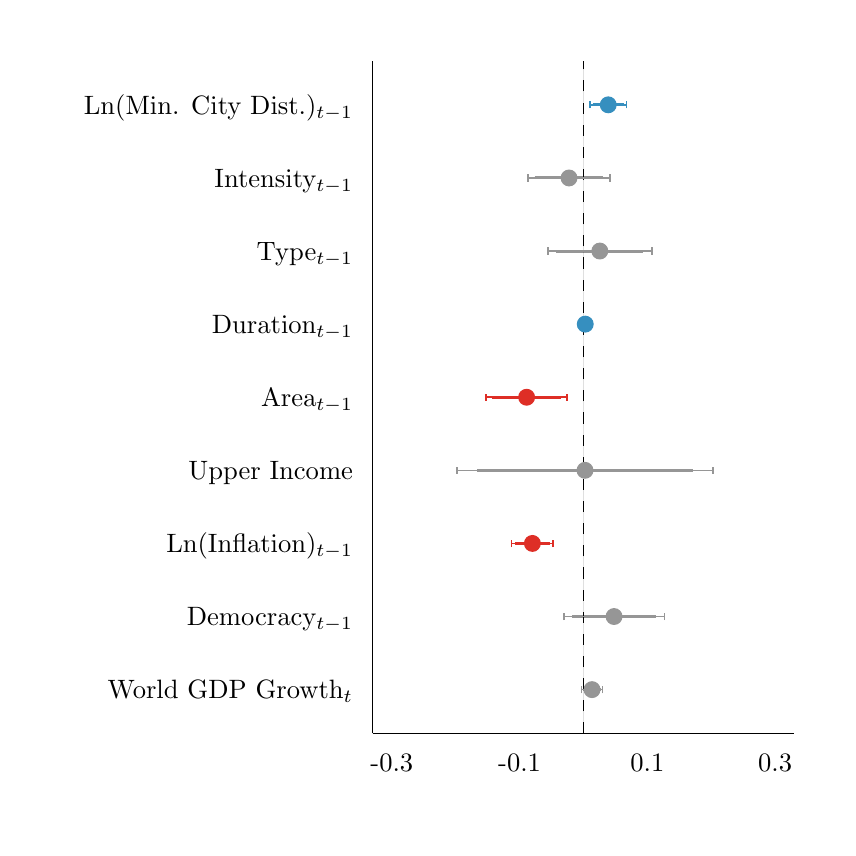
\begin{tikzpicture}[x=1pt,y=1pt]
\definecolor[named]{fillColor}{rgb}{1.00,1.00,1.00}
\path[use as bounding box,fill=fillColor,fill opacity=0.00] (0,0) rectangle (289.08,289.08);
\begin{scope}
\path[clip] (  0.00,  0.00) rectangle (289.08,289.08);
\definecolor[named]{drawColor}{rgb}{1.00,1.00,1.00}
\definecolor[named]{fillColor}{rgb}{1.00,1.00,1.00}

\path[draw=drawColor,line width= 0.6pt,line join=round,line cap=round,fill=fillColor] ( -0.00,  0.00) rectangle (289.08,289.08);
\end{scope}
\begin{scope}
\path[clip] (124.66, 34.03) rectangle (277.03,277.03);
\definecolor[named]{fillColor}{rgb}{1.00,1.00,1.00}

\path[fill=fillColor] (124.66, 34.03) rectangle (277.04,277.03);
\definecolor[named]{drawColor}{rgb}{0.59,0.59,0.59}
\definecolor[named]{fillColor}{rgb}{0.59,0.59,0.59}

\path[draw=drawColor,draw opacity=0.30,line width= 0.3pt,line join=round,fill=fillColor,fill opacity=0.30] (200.10, 49.88) -- (207.76, 49.88);

\path[draw=drawColor,draw opacity=0.30,line width= 0.3pt,line join=round,fill=fillColor,fill opacity=0.30] (193.68, 76.30) -- (230.11, 76.30);
\definecolor[named]{drawColor}{rgb}{0.87,0.18,0.15}
\definecolor[named]{fillColor}{rgb}{0.87,0.18,0.15}

\path[draw=drawColor,draw opacity=0.30,line width= 0.3pt,line join=round,fill=fillColor,fill opacity=0.30] (174.88,102.71) -- (189.88,102.71);
\definecolor[named]{drawColor}{rgb}{0.59,0.59,0.59}
\definecolor[named]{fillColor}{rgb}{0.59,0.59,0.59}

\path[draw=drawColor,draw opacity=0.30,line width= 0.3pt,line join=round,fill=fillColor,fill opacity=0.30] (155.06,129.12) -- (247.73,129.12);
\definecolor[named]{drawColor}{rgb}{0.87,0.18,0.15}
\definecolor[named]{fillColor}{rgb}{0.87,0.18,0.15}

\path[draw=drawColor,draw opacity=0.30,line width= 0.3pt,line join=round,fill=fillColor,fill opacity=0.30] (165.59,155.53) -- (195.00,155.53);
\definecolor[named]{drawColor}{rgb}{0.21,0.56,0.75}
\definecolor[named]{fillColor}{rgb}{0.21,0.56,0.75}

\path[draw=drawColor,draw opacity=0.30,line width= 0.3pt,line join=round,fill=fillColor,fill opacity=0.30] (200.88,181.95) -- (202.07,181.95);
\definecolor[named]{drawColor}{rgb}{0.59,0.59,0.59}
\definecolor[named]{fillColor}{rgb}{0.59,0.59,0.59}

\path[draw=drawColor,draw opacity=0.30,line width= 0.3pt,line join=round,fill=fillColor,fill opacity=0.30] (187.98,208.36) -- (225.50,208.36);

\path[draw=drawColor,draw opacity=0.30,line width= 0.3pt,line join=round,fill=fillColor,fill opacity=0.30] (180.79,234.77) -- (210.45,234.77);
\definecolor[named]{drawColor}{rgb}{0.21,0.56,0.75}
\definecolor[named]{fillColor}{rgb}{0.21,0.56,0.75}

\path[draw=drawColor,draw opacity=0.30,line width= 0.3pt,line join=round,fill=fillColor,fill opacity=0.30] (203.18,261.19) -- (216.39,261.19);
\definecolor[named]{drawColor}{rgb}{0.59,0.59,0.59}
\definecolor[named]{fillColor}{rgb}{0.59,0.59,0.59}

\path[draw=drawColor,line width= 1.1pt,line join=round,fill=fillColor] (200.72, 49.88) -- (207.15, 49.88);

\path[draw=drawColor,line width= 1.1pt,line join=round,fill=fillColor] (196.61, 76.30) -- (227.18, 76.30);
\definecolor[named]{drawColor}{rgb}{0.87,0.18,0.15}
\definecolor[named]{fillColor}{rgb}{0.87,0.18,0.15}

\path[draw=drawColor,line width= 1.1pt,line join=round,fill=fillColor] (176.09,102.71) -- (188.68,102.71);
\definecolor[named]{drawColor}{rgb}{0.59,0.59,0.59}
\definecolor[named]{fillColor}{rgb}{0.59,0.59,0.59}

\path[draw=drawColor,line width= 1.1pt,line join=round,fill=fillColor] (162.51,129.12) -- (240.28,129.12);
\definecolor[named]{drawColor}{rgb}{0.87,0.18,0.15}
\definecolor[named]{fillColor}{rgb}{0.87,0.18,0.15}

\path[draw=drawColor,line width= 1.1pt,line join=round,fill=fillColor] (167.95,155.53) -- (192.63,155.53);
\definecolor[named]{drawColor}{rgb}{0.21,0.56,0.75}
\definecolor[named]{fillColor}{rgb}{0.21,0.56,0.75}

\path[draw=drawColor,line width= 1.1pt,line join=round,fill=fillColor] (200.97,181.95) -- (201.98,181.95);
\definecolor[named]{drawColor}{rgb}{0.59,0.59,0.59}
\definecolor[named]{fillColor}{rgb}{0.59,0.59,0.59}

\path[draw=drawColor,line width= 1.1pt,line join=round,fill=fillColor] (191.00,208.36) -- (222.48,208.36);

\path[draw=drawColor,line width= 1.1pt,line join=round,fill=fillColor] (183.17,234.77) -- (208.07,234.77);
\definecolor[named]{drawColor}{rgb}{0.21,0.56,0.75}
\definecolor[named]{fillColor}{rgb}{0.21,0.56,0.75}

\path[draw=drawColor,line width= 1.1pt,line join=round,fill=fillColor] (204.24,261.19) -- (215.33,261.19);
\definecolor[named]{drawColor}{rgb}{0.00,0.00,0.00}
\definecolor[named]{fillColor}{rgb}{0.00,0.00,0.00}

\path[draw=drawColor,line width= 0.6pt,dash pattern=on 4pt off 4pt ,line join=round,fill=fillColor] (200.85, 34.03) -- (200.85,277.03);
\definecolor[named]{drawColor}{rgb}{0.21,0.56,0.75}
\definecolor[named]{fillColor}{rgb}{0.21,0.56,0.75}

\path[draw=drawColor,line width= 0.4pt,line join=round,line cap=round,fill=fillColor] (209.79,261.19) circle (  2.85);
\definecolor[named]{drawColor}{rgb}{0.59,0.59,0.59}
\definecolor[named]{fillColor}{rgb}{0.59,0.59,0.59}

\path[draw=drawColor,line width= 0.4pt,line join=round,line cap=round,fill=fillColor] (195.62,234.77) circle (  2.85);

\path[draw=drawColor,line width= 0.4pt,line join=round,line cap=round,fill=fillColor] (206.74,208.36) circle (  2.85);
\definecolor[named]{drawColor}{rgb}{0.21,0.56,0.75}
\definecolor[named]{fillColor}{rgb}{0.21,0.56,0.75}

\path[draw=drawColor,line width= 0.4pt,line join=round,line cap=round,fill=fillColor] (201.47,181.95) circle (  2.85);
\definecolor[named]{drawColor}{rgb}{0.87,0.18,0.15}
\definecolor[named]{fillColor}{rgb}{0.87,0.18,0.15}

\path[draw=drawColor,line width= 0.4pt,line join=round,line cap=round,fill=fillColor] (180.29,155.53) circle (  2.85);
\definecolor[named]{drawColor}{rgb}{0.59,0.59,0.59}
\definecolor[named]{fillColor}{rgb}{0.59,0.59,0.59}

\path[draw=drawColor,line width= 0.4pt,line join=round,line cap=round,fill=fillColor] (201.39,129.12) circle (  2.85);
\definecolor[named]{drawColor}{rgb}{0.87,0.18,0.15}
\definecolor[named]{fillColor}{rgb}{0.87,0.18,0.15}

\path[draw=drawColor,line width= 0.4pt,line join=round,line cap=round,fill=fillColor] (182.38,102.71) circle (  2.85);
\definecolor[named]{drawColor}{rgb}{0.59,0.59,0.59}
\definecolor[named]{fillColor}{rgb}{0.59,0.59,0.59}

\path[draw=drawColor,line width= 0.4pt,line join=round,line cap=round,fill=fillColor] (211.89, 76.30) circle (  2.85);

\path[draw=drawColor,line width= 0.4pt,line join=round,line cap=round,fill=fillColor] (203.93, 49.88) circle (  2.85);

\path[draw=drawColor,line width= 0.6pt,line join=round] (207.76, 48.56) --
	(207.76, 51.20);

\path[draw=drawColor,line width= 0.6pt,line join=round] (207.76, 49.88) --
	(200.10, 49.88);

\path[draw=drawColor,line width= 0.6pt,line join=round] (200.10, 48.56) --
	(200.10, 51.20);

\path[draw=drawColor,line width= 0.6pt,line join=round] (230.11, 74.97) --
	(230.11, 77.62);

\path[draw=drawColor,line width= 0.6pt,line join=round] (230.11, 76.30) --
	(193.68, 76.30);

\path[draw=drawColor,line width= 0.6pt,line join=round] (193.68, 74.97) --
	(193.68, 77.62);
\definecolor[named]{drawColor}{rgb}{0.87,0.18,0.15}

\path[draw=drawColor,line width= 0.6pt,line join=round] (189.88,101.39) --
	(189.88,104.03);

\path[draw=drawColor,line width= 0.6pt,line join=round] (189.88,102.71) --
	(174.88,102.71);

\path[draw=drawColor,line width= 0.6pt,line join=round] (174.88,101.39) --
	(174.88,104.03);
\definecolor[named]{drawColor}{rgb}{0.59,0.59,0.59}

\path[draw=drawColor,line width= 0.6pt,line join=round] (247.73,127.80) --
	(247.73,130.44);

\path[draw=drawColor,line width= 0.6pt,line join=round] (247.73,129.12) --
	(155.06,129.12);

\path[draw=drawColor,line width= 0.6pt,line join=round] (155.06,127.80) --
	(155.06,130.44);
\definecolor[named]{drawColor}{rgb}{0.87,0.18,0.15}

\path[draw=drawColor,line width= 0.6pt,line join=round] (195.00,154.21) --
	(195.00,156.86);

\path[draw=drawColor,line width= 0.6pt,line join=round] (195.00,155.53) --
	(165.59,155.53);

\path[draw=drawColor,line width= 0.6pt,line join=round] (165.59,154.21) --
	(165.59,156.86);
\definecolor[named]{drawColor}{rgb}{0.21,0.56,0.75}

\path[draw=drawColor,line width= 0.6pt,line join=round] (202.07,180.63) --
	(202.07,183.27);

\path[draw=drawColor,line width= 0.6pt,line join=round] (202.07,181.95) --
	(200.88,181.95);

\path[draw=drawColor,line width= 0.6pt,line join=round] (200.88,180.63) --
	(200.88,183.27);
\definecolor[named]{drawColor}{rgb}{0.59,0.59,0.59}

\path[draw=drawColor,line width= 0.6pt,line join=round] (225.50,207.04) --
	(225.50,209.68);

\path[draw=drawColor,line width= 0.6pt,line join=round] (225.50,208.36) --
	(187.98,208.36);

\path[draw=drawColor,line width= 0.6pt,line join=round] (187.98,207.04) --
	(187.98,209.68);

\path[draw=drawColor,line width= 0.6pt,line join=round] (210.45,233.45) --
	(210.45,236.09);

\path[draw=drawColor,line width= 0.6pt,line join=round] (210.45,234.77) --
	(180.79,234.77);

\path[draw=drawColor,line width= 0.6pt,line join=round] (180.79,233.45) --
	(180.79,236.09);
\definecolor[named]{drawColor}{rgb}{0.21,0.56,0.75}

\path[draw=drawColor,line width= 0.6pt,line join=round] (216.39,259.87) --
	(216.39,262.51);

\path[draw=drawColor,line width= 0.6pt,line join=round] (216.39,261.19) --
	(203.18,261.19);

\path[draw=drawColor,line width= 0.6pt,line join=round] (203.18,259.87) --
	(203.18,262.51);
\end{scope}
\begin{scope}
\path[clip] (  0.00,  0.00) rectangle (289.08,289.08);
\definecolor[named]{drawColor}{rgb}{0.00,0.00,0.00}

\path[draw=drawColor,line width= 0.6pt,line join=round] (124.66, 34.03) --
	(124.66,277.03);
\end{scope}
\begin{scope}
\path[clip] (  0.00,  0.00) rectangle (289.08,289.08);
\definecolor[named]{drawColor}{rgb}{0.00,0.00,0.00}

\node[text=drawColor,anchor=base east,inner sep=0pt, outer sep=0pt, scale=  0.96] at (117.55, 46.58) {World GDP Growth$_{t}$};

\node[text=drawColor,anchor=base east,inner sep=0pt, outer sep=0pt, scale=  0.96] at (117.55, 72.99) {Democracy$_{t-1}$};

\node[text=drawColor,anchor=base east,inner sep=0pt, outer sep=0pt, scale=  0.96] at (117.55, 99.40) {Ln(Inflation)$_{t-1}$};

\node[text=drawColor,anchor=base east,inner sep=0pt, outer sep=0pt, scale=  0.96] at (117.55,125.82) {Upper Income};

\node[text=drawColor,anchor=base east,inner sep=0pt, outer sep=0pt, scale=  0.96] at (117.55,152.23) {Area$_{t-1}$};

\node[text=drawColor,anchor=base east,inner sep=0pt, outer sep=0pt, scale=  0.96] at (117.55,178.64) {Duration$_{t-1}$};

\node[text=drawColor,anchor=base east,inner sep=0pt, outer sep=0pt, scale=  0.96] at (117.55,205.06) {Type$_{t-1}$};

\node[text=drawColor,anchor=base east,inner sep=0pt, outer sep=0pt, scale=  0.96] at (117.55,231.47) {Intensity$_{t-1}$};

\node[text=drawColor,anchor=base east,inner sep=0pt, outer sep=0pt, scale=  0.96] at (117.55,257.88) {Ln(Min. City Dist.)$_{t-1}$};
\end{scope}
\begin{scope}
\path[clip] (  0.00,  0.00) rectangle (289.08,289.08);
\definecolor[named]{drawColor}{rgb}{0.00,0.00,0.00}

\path[draw=drawColor,line width= 0.6pt,line join=round] (124.66, 34.03) --
	(277.03, 34.03);
\end{scope}
\begin{scope}
\path[clip] (  0.00,  0.00) rectangle (289.08,289.08);
\definecolor[named]{drawColor}{rgb}{0.00,0.00,0.00}

\node[text=drawColor,anchor=base,inner sep=0pt, outer sep=0pt, scale=  0.96] at (131.59, 20.31) {-0.3};

\node[text=drawColor,anchor=base,inner sep=0pt, outer sep=0pt, scale=  0.96] at (177.76, 20.31) {-0.1};

\node[text=drawColor,anchor=base,inner sep=0pt, outer sep=0pt, scale=  0.96] at (223.94, 20.31) {0.1};

\node[text=drawColor,anchor=base,inner sep=0pt, outer sep=0pt, scale=  0.96] at (270.11, 20.31) {0.3};
\end{scope}
\end{tikzpicture}
}
		\label{fig:cityCoef}}
	\end{tabular}
	\caption{Regression results using conflict distance from capital city on the left, and the chart on the right shows regression results using minimum conflict distance from any major city. Darker colors indicates that the coefficient estimate is significantly different from zero at a 95\% CI, while lighter the same for a 90\% CI. Grey indicates that the estimate is not significantly different from zero at either of those intervals.}
	\label{fig:coefplot}
\end{figure}

To assess the substantive effect of the minimum conflict distance variable we conduct a number of simulations. We set up scenarios where we hold all variables to their median except for the logged, minimum conflict distance, which we range from its minimum to maximum value. Next, we conduct 1,000 random draws from a multivariate normal to obtain distributions for the point estimates of each of the regression coefficients. After obtaining these distributions, we calculate the predicted value of GDP growth based on the conditions set by the scenarios. We plot the results of this analyis in figure \ref{fig:simsPlot}.  

\begin{figure}
	\centering
	\begin{tabular}{cc}
		\subfloat[SubFigure 1][Capital City]{
			\resizebox{.45\textwidth}{!}{% Created by tikzDevice version 0.7.0 on 2014-10-06 20:10:12
% !TEX encoding = UTF-8 Unicode
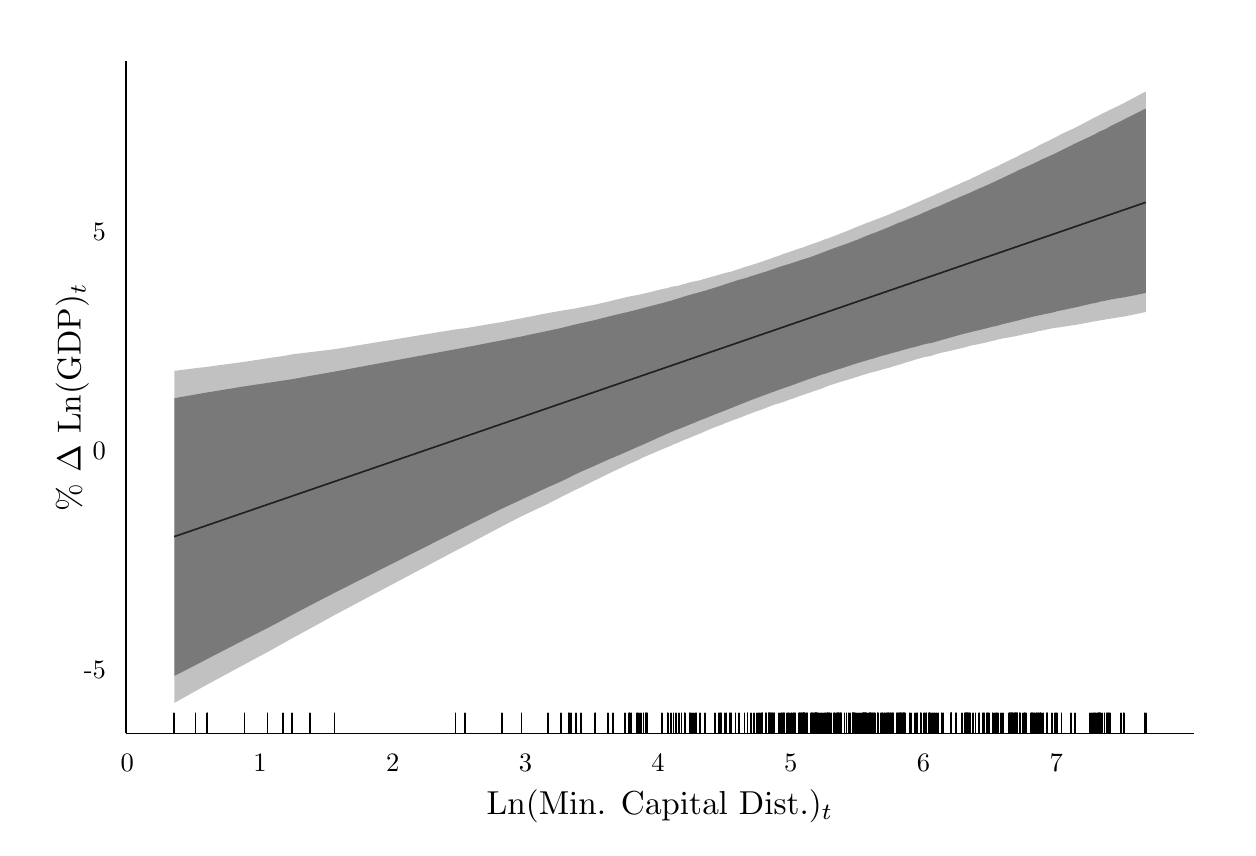
\begin{tikzpicture}[x=1pt,y=1pt]
\definecolor[named]{fillColor}{rgb}{1.00,1.00,1.00}
\path[use as bounding box,fill=fillColor,fill opacity=0.00] (0,0) rectangle (433.62,289.08);
\begin{scope}
\path[clip] (  0.00,  0.00) rectangle (433.62,289.08);
\definecolor[named]{drawColor}{rgb}{1.00,1.00,1.00}
\definecolor[named]{fillColor}{rgb}{1.00,1.00,1.00}

\path[draw=drawColor,line width= 0.6pt,line join=round,line cap=round,fill=fillColor] (  0.00,  0.00) rectangle (433.62,289.08);
\end{scope}
\begin{scope}
\path[clip] ( 35.42, 34.03) rectangle (421.57,277.03);
\definecolor[named]{fillColor}{rgb}{1.00,1.00,1.00}

\path[fill=fillColor] ( 35.42, 34.03) rectangle (421.57,277.03);
\definecolor[named]{drawColor}{rgb}{0.00,0.00,0.00}

\path[draw=drawColor,line width= 0.6pt,line join=round] ( 52.97,105.17) --
	( 60.61,107.79) --
	( 64.85,109.25) --
	( 64.98,109.30) --
	( 78.30,113.88) --
	( 86.71,116.78) --
	( 92.34,118.71) --
	( 95.59,119.83) --
	(101.92,122.01) --
	(110.88,125.09) --
	(154.64,140.15) --
	(158.01,141.31) --
	(171.43,145.93) --
	(178.49,148.35) --
	(187.92,151.60) --
	(192.71,153.25) --
	(195.62,154.25) --
	(195.71,154.28) --
	(196.35,154.50) --
	(198.04,155.08) --
	(199.87,155.71) --
	(204.99,157.47) --
	(205.19,157.54) --
	(209.65,159.08) --
	(211.50,159.71) --
	(215.87,161.22) --
	(217.33,161.72) --
	(217.43,161.75) --
	(217.68,161.84) --
	(218.17,162.01) --
	(220.17,162.70) --
	(220.33,162.75) --
	(220.93,162.96) --
	(221.63,163.20) --
	(222.58,163.53) --
	(223.29,163.77) --
	(223.54,163.86) --
	(223.59,163.87) --
	(224.00,164.02) --
	(229.14,165.78) --
	(231.15,166.48) --
	(231.34,166.54) --
	(232.39,166.90) --
	(233.34,167.23) --
	(234.24,167.54) --
	(235.24,167.88) --
	(236.22,168.22) --
	(237.40,168.63) --
	(237.41,168.63) --
	(239.29,169.28) --
	(239.31,169.28) --
	(240.03,169.53) --
	(240.80,169.79) --
	(241.27,169.96) --
	(241.65,170.09) --
	(242.95,170.54) --
	(244.78,171.17) --
	(248.30,172.38) --
	(249.74,172.87) --
	(250.22,173.04) --
	(250.38,173.09) --
	(250.69,173.20) --
	(251.97,173.64) --
	(252.46,173.81) --
	(253.69,174.23) --
	(253.89,174.30) --
	(254.34,174.45) --
	(255.73,174.94) --
	(256.94,175.35) --
	(258.99,176.06) --
	(260.08,176.43) --
	(260.16,176.46) --
	(261.39,176.88) --
	(262.57,177.29) --
	(263.47,177.60) --
	(264.14,177.83) --
	(264.43,177.93) --
	(264.94,178.10) --
	(265.11,178.16) --
	(265.48,178.29) --
	(265.54,178.31) --
	(266.69,178.71) --
	(266.70,178.71) --
	(267.74,179.07) --
	(267.83,179.10) --
	(267.95,179.14) --
	(268.15,179.21) --
	(268.32,179.26) --
	(268.51,179.33) --
	(268.75,179.41) --
	(269.12,179.54) --
	(269.30,179.60) --
	(269.75,179.76) --
	(269.91,179.81) --
	(271.51,180.36) --
	(272.31,180.64) --
	(272.40,180.67) --
	(272.91,180.84) --
	(273.01,180.88) --
	(273.29,180.98) --
	(273.48,181.04) --
	(274.31,181.33) --
	(274.85,181.51) --
	(274.88,181.52) --
	(275.50,181.74) --
	(276.03,181.92) --
	(276.14,181.95) --
	(276.73,182.16) --
	(276.77,182.17) --
	(277.28,182.35) --
	(277.37,182.38) --
	(278.83,182.88) --
	(278.93,182.92) --
	(278.99,182.94) --
	(279.03,182.95) --
	(279.36,183.06) --
	(279.83,183.23) --
	(279.90,183.25) --
	(280.21,183.36) --
	(280.36,183.41) --
	(280.41,183.43) --
	(280.47,183.45) --
	(280.50,183.46) --
	(280.60,183.49) --
	(280.63,183.50) --
	(281.16,183.68) --
	(281.52,183.81) --
	(281.60,183.84) --
	(283.10,184.35) --
	(283.28,184.41) --
	(283.34,184.44) --
	(283.74,184.57) --
	(283.80,184.59) --
	(284.26,184.75) --
	(284.43,184.81) --
	(284.75,184.92) --
	(284.80,184.94) --
	(284.81,184.94) --
	(284.81,184.94) --
	(284.84,184.95) --
	(284.88,184.96) --
	(285.44,185.16) --
	(285.67,185.24) --
	(286.04,185.36) --
	(286.70,185.59) --
	(286.95,185.68) --
	(287.76,185.96) --
	(288.16,186.09) --
	(288.45,186.19) --
	(288.86,186.33) --
	(289.03,186.39) --
	(289.13,186.43) --
	(289.30,186.48) --
	(289.61,186.59) --
	(289.71,186.63) --
	(289.99,186.72) --
	(290.44,186.88) --
	(291.29,187.17) --
	(291.45,187.22) --
	(291.58,187.27) --
	(292.20,187.48) --
	(292.36,187.54) --
	(292.77,187.68) --
	(292.78,187.68) --
	(292.85,187.71) --
	(292.94,187.74) --
	(293.49,187.93) --
	(293.61,187.97) --
	(293.90,188.07) --
	(293.94,188.08) --
	(295.12,188.49) --
	(295.85,188.74) --
	(296.61,189.00) --
	(297.11,189.17) --
	(297.99,189.47) --
	(298.09,189.51) --
	(298.13,189.52) --
	(298.21,189.55) --
	(298.45,189.63) --
	(298.48,189.64) --
	(298.71,189.72) --
	(298.89,189.79) --
	(299.22,189.90) --
	(300.07,190.19) --
	(300.69,190.40) --
	(301.34,190.63) --
	(301.81,190.79) --
	(301.86,190.81) --
	(302.06,190.87) --
	(302.08,190.88) --
	(302.20,190.93) --
	(302.30,190.96) --
	(302.45,191.01) --
	(302.52,191.03) --
	(302.61,191.06) --
	(302.89,191.16) --
	(302.93,191.17) --
	(303.17,191.26) --
	(304.10,191.58) --
	(304.31,191.65) --
	(304.47,191.71) --
	(304.48,191.71) --
	(304.60,191.75) --
	(304.68,191.78) --
	(305.11,191.93) --
	(305.28,191.98) --
	(305.76,192.15) --
	(305.86,192.18) --
	(306.15,192.28) --
	(307.03,192.59) --
	(307.16,192.63) --
	(307.37,192.70) --
	(308.42,193.06) --
	(308.63,193.14) --
	(308.79,193.19) --
	(309.08,193.29) --
	(309.55,193.45) --
	(309.72,193.51) --
	(310.36,193.73) --
	(310.45,193.76) --
	(310.80,193.88) --
	(310.98,193.95) --
	(311.09,193.98) --
	(311.49,194.12) --
	(311.71,194.20) --
	(311.87,194.25) --
	(312.39,194.43) --
	(312.68,194.53) --
	(312.75,194.55) --
	(314.09,195.02) --
	(314.12,195.02) --
	(314.55,195.17) --
	(314.84,195.27) --
	(315.05,195.34) --
	(315.28,195.42) --
	(315.54,195.51) --
	(315.61,195.54) --
	(315.65,195.55) --
	(316.29,195.77) --
	(316.37,195.80) --
	(316.58,195.87) --
	(316.61,195.88) --
	(316.72,195.92) --
	(317.13,196.06) --
	(318.60,196.57) --
	(319.14,196.75) --
	(320.71,197.29) --
	(321.34,197.51) --
	(321.47,197.55) --
	(322.56,197.93) --
	(322.64,197.96) --
	(322.93,198.06) --
	(323.98,198.42) --
	(324.06,198.44) --
	(324.53,198.61) --
	(324.82,198.71) --
	(325.46,198.93) --
	(325.85,199.06) --
	(325.87,199.07) --
	(325.91,199.08) --
	(326.16,199.17) --
	(326.46,199.27) --
	(327.01,199.46) --
	(327.50,199.63) --
	(327.78,199.72) --
	(328.37,199.93) --
	(328.92,200.12) --
	(330.17,200.55) --
	(330.38,200.62) --
	(330.88,200.79) --
	(333.53,201.71) --
	(333.56,201.71) --
	(333.69,201.76) --
	(333.82,201.80) --
	(333.83,201.81) --
	(335.38,202.34) --
	(335.47,202.37) --
	(337.65,203.12) --
	(338.50,203.41) --
	(338.83,203.53) --
	(338.87,203.54) --
	(339.04,203.60) --
	(339.21,203.66) --
	(339.40,203.72) --
	(339.55,203.77) --
	(339.76,203.85) --
	(339.84,203.88) --
	(340.15,203.98) --
	(340.28,204.03) --
	(340.65,204.15) --
	(341.52,204.45) --
	(342.53,204.80) --
	(343.79,205.23) --
	(343.95,205.29) --
	(345.11,205.69) --
	(345.20,205.72) --
	(345.78,205.92) --
	(346.49,206.16) --
	(346.80,206.27) --
	(346.94,206.32) --
	(347.30,206.44) --
	(348.63,206.90) --
	(348.84,206.97) --
	(349.59,207.23) --
	(350.01,207.38) --
	(350.27,207.46) --
	(350.57,207.57) --
	(351.61,207.93) --
	(352.50,208.23) --
	(354.60,208.95) --
	(354.77,209.01) --
	(355.03,209.10) --
	(355.06,209.11) --
	(355.38,209.22) --
	(355.44,209.24) --
	(355.66,209.32) --
	(355.69,209.33) --
	(356.06,209.46) --
	(356.08,209.46) --
	(356.57,209.63) --
	(356.86,209.73) --
	(356.99,209.78) --
	(357.04,209.79) --
	(357.10,209.81) --
	(357.28,209.88) --
	(357.68,210.01) --
	(357.71,210.02) --
	(358.36,210.25) --
	(358.45,210.28) --
	(358.80,210.40) --
	(359.58,210.67) --
	(360.14,210.86) --
	(360.17,210.87) --
	(360.28,210.91) --
	(360.68,211.05) --
	(362.54,211.69) --
	(362.92,211.82) --
	(362.99,211.84) --
	(362.99,211.84) --
	(363.68,212.08) --
	(363.71,212.09) --
	(364.25,212.28) --
	(364.57,212.39) --
	(364.77,212.45) --
	(365.00,212.53) --
	(365.26,212.62) --
	(365.84,212.82) --
	(365.84,212.82) --
	(365.92,212.85) --
	(366.04,212.89) --
	(366.47,213.04) --
	(367.05,213.24) --
	(368.20,213.63) --
	(368.39,213.70) --
	(368.50,213.74) --
	(370.21,214.32) --
	(371.17,214.65) --
	(371.58,214.80) --
	(372.02,214.95) --
	(373.58,215.48) --
	(376.96,216.65) --
	(378.52,217.19) --
	(383.85,219.02) --
	(384.44,219.22) --
	(384.92,219.39) --
	(385.30,219.52) --
	(385.73,219.66) --
	(385.96,219.74) --
	(386.70,220.00) --
	(386.81,220.04) --
	(387.17,220.16) --
	(387.19,220.17) --
	(387.24,220.18) --
	(387.39,220.24) --
	(387.67,220.34) --
	(388.26,220.54) --
	(389.16,220.85) --
	(389.82,221.07) --
	(390.40,221.27) --
	(390.44,221.29) --
	(390.79,221.41) --
	(391.07,221.50) --
	(395.16,222.91) --
	(396.00,223.20) --
	(396.15,223.25) --
	(403.52,225.79) --
	(404.02,225.96);
\definecolor[named]{fillColor}{rgb}{0.20,0.20,0.20}

\path[fill=fillColor,fill opacity=0.30] ( 52.97,165.07) --
	( 60.61,166.03) --
	( 64.85,166.51) --
	( 64.98,166.54) --
	( 78.30,168.33) --
	( 86.71,169.61) --
	( 92.34,170.44) --
	( 95.59,171.03) --
	(101.92,171.81) --
	(110.88,172.89) --
	(154.64,180.05) --
	(158.01,180.45) --
	(171.43,182.73) --
	(178.49,184.08) --
	(187.92,185.93) --
	(192.71,186.77) --
	(195.62,187.27) --
	(195.71,187.28) --
	(196.35,187.38) --
	(198.04,187.65) --
	(199.87,188.05) --
	(204.99,189.01) --
	(205.19,189.03) --
	(209.65,190.06) --
	(211.50,190.52) --
	(215.87,191.59) --
	(217.33,191.90) --
	(217.43,191.93) --
	(217.68,191.97) --
	(218.17,192.07) --
	(220.17,192.44) --
	(220.33,192.49) --
	(220.93,192.59) --
	(221.63,192.75) --
	(222.58,192.98) --
	(223.29,193.13) --
	(223.54,193.18) --
	(223.59,193.19) --
	(224.00,193.30) --
	(229.14,194.56) --
	(231.15,194.97) --
	(231.34,194.99) --
	(232.39,195.37) --
	(233.34,195.60) --
	(234.24,195.69) --
	(235.24,195.85) --
	(236.22,196.18) --
	(237.40,196.49) --
	(237.41,196.49) --
	(239.29,197.05) --
	(239.31,197.06) --
	(240.03,197.23) --
	(240.80,197.39) --
	(241.27,197.46) --
	(241.65,197.55) --
	(242.95,197.83) --
	(244.78,198.38) --
	(248.30,199.35) --
	(249.74,199.77) --
	(250.22,199.91) --
	(250.38,199.94) --
	(250.69,200.06) --
	(251.97,200.42) --
	(252.46,200.53) --
	(253.69,200.79) --
	(253.89,200.86) --
	(254.34,200.96) --
	(255.73,201.43) --
	(256.94,201.82) --
	(258.99,202.54) --
	(260.08,202.88) --
	(260.16,202.90) --
	(261.39,203.25) --
	(262.57,203.64) --
	(263.47,203.91) --
	(264.14,204.11) --
	(264.43,204.22) --
	(264.94,204.38) --
	(265.11,204.45) --
	(265.48,204.57) --
	(265.54,204.59) --
	(266.69,205.01) --
	(266.70,205.01) --
	(267.74,205.35) --
	(267.83,205.37) --
	(267.95,205.45) --
	(268.15,205.52) --
	(268.32,205.56) --
	(268.51,205.63) --
	(268.75,205.74) --
	(269.12,205.89) --
	(269.30,205.97) --
	(269.75,206.12) --
	(269.91,206.17) --
	(271.51,206.69) --
	(272.31,207.01) --
	(272.40,207.06) --
	(272.91,207.29) --
	(273.01,207.33) --
	(273.29,207.43) --
	(273.48,207.49) --
	(274.31,207.72) --
	(274.85,207.89) --
	(274.88,207.90) --
	(275.50,208.11) --
	(276.03,208.30) --
	(276.14,208.34) --
	(276.73,208.55) --
	(276.77,208.57) --
	(277.28,208.75) --
	(277.37,208.78) --
	(278.83,209.26) --
	(278.93,209.30) --
	(278.99,209.33) --
	(279.03,209.34) --
	(279.36,209.43) --
	(279.83,209.54) --
	(279.90,209.57) --
	(280.21,209.70) --
	(280.36,209.75) --
	(280.41,209.78) --
	(280.47,209.80) --
	(280.50,209.81) --
	(280.60,209.85) --
	(280.63,209.85) --
	(281.16,210.05) --
	(281.52,210.20) --
	(281.60,210.24) --
	(283.10,210.77) --
	(283.28,210.82) --
	(283.34,210.83) --
	(283.74,210.94) --
	(283.80,210.97) --
	(284.26,211.19) --
	(284.43,211.24) --
	(284.75,211.33) --
	(284.80,211.34) --
	(284.81,211.34) --
	(284.81,211.34) --
	(284.84,211.35) --
	(284.88,211.37) --
	(285.44,211.54) --
	(285.67,211.63) --
	(286.04,211.78) --
	(286.70,212.02) --
	(286.95,212.12) --
	(287.76,212.51) --
	(288.16,212.63) --
	(288.45,212.70) --
	(288.86,212.81) --
	(289.03,212.87) --
	(289.13,212.93) --
	(289.30,212.99) --
	(289.61,213.12) --
	(289.71,213.16) --
	(289.99,213.26) --
	(290.44,213.43) --
	(291.29,213.72) --
	(291.45,213.79) --
	(291.58,213.85) --
	(292.20,214.08) --
	(292.36,214.13) --
	(292.77,214.30) --
	(292.78,214.30) --
	(292.85,214.32) --
	(292.94,214.36) --
	(293.49,214.59) --
	(293.61,214.64) --
	(293.90,214.77) --
	(293.94,214.79) --
	(295.12,215.21) --
	(295.85,215.51) --
	(296.61,215.83) --
	(297.11,216.04) --
	(297.99,216.40) --
	(298.09,216.45) --
	(298.13,216.47) --
	(298.21,216.50) --
	(298.45,216.60) --
	(298.48,216.61) --
	(298.71,216.72) --
	(298.89,216.80) --
	(299.22,216.90) --
	(300.07,217.25) --
	(300.69,217.51) --
	(301.34,217.77) --
	(301.81,217.95) --
	(301.86,217.97) --
	(302.06,218.06) --
	(302.08,218.06) --
	(302.20,218.12) --
	(302.30,218.16) --
	(302.45,218.22) --
	(302.52,218.25) --
	(302.61,218.29) --
	(302.89,218.40) --
	(302.93,218.42) --
	(303.17,218.52) --
	(304.10,218.84) --
	(304.31,218.92) --
	(304.47,218.97) --
	(304.48,218.97) --
	(304.60,219.01) --
	(304.68,219.04) --
	(305.11,219.23) --
	(305.28,219.30) --
	(305.76,219.46) --
	(305.86,219.49) --
	(306.15,219.58) --
	(307.03,219.96) --
	(307.16,220.02) --
	(307.37,220.07) --
	(308.42,220.47) --
	(308.63,220.55) --
	(308.79,220.61) --
	(309.08,220.73) --
	(309.55,220.92) --
	(309.72,220.98) --
	(310.36,221.22) --
	(310.45,221.25) --
	(310.80,221.37) --
	(310.98,221.46) --
	(311.09,221.48) --
	(311.49,221.66) --
	(311.71,221.78) --
	(311.87,221.84) --
	(312.39,222.06) --
	(312.68,222.19) --
	(312.75,222.21) --
	(314.09,222.81) --
	(314.12,222.82) --
	(314.55,223.00) --
	(314.84,223.11) --
	(315.05,223.18) --
	(315.28,223.25) --
	(315.54,223.34) --
	(315.61,223.36) --
	(315.65,223.37) --
	(316.29,223.65) --
	(316.37,223.69) --
	(316.58,223.78) --
	(316.61,223.79) --
	(316.72,223.82) --
	(317.13,223.99) --
	(318.60,224.64) --
	(319.14,224.92) --
	(320.71,225.62) --
	(321.34,225.89) --
	(321.47,225.94) --
	(322.56,226.40) --
	(322.64,226.44) --
	(322.93,226.57) --
	(323.98,227.03) --
	(324.06,227.07) --
	(324.53,227.28) --
	(324.82,227.40) --
	(325.46,227.67) --
	(325.85,227.84) --
	(325.87,227.86) --
	(325.91,227.88) --
	(326.16,227.97) --
	(326.46,228.10) --
	(327.01,228.35) --
	(327.50,228.52) --
	(327.78,228.67) --
	(328.37,228.96) --
	(328.92,229.20) --
	(330.17,229.74) --
	(330.38,229.85) --
	(330.88,230.08) --
	(333.53,231.22) --
	(333.56,231.23) --
	(333.69,231.29) --
	(333.82,231.35) --
	(333.83,231.35) --
	(335.38,232.05) --
	(335.47,232.09) --
	(337.65,233.08) --
	(338.50,233.45) --
	(338.83,233.59) --
	(338.87,233.61) --
	(339.04,233.68) --
	(339.21,233.75) --
	(339.40,233.82) --
	(339.55,233.88) --
	(339.76,233.97) --
	(339.84,234.00) --
	(340.15,234.13) --
	(340.28,234.18) --
	(340.65,234.38) --
	(341.52,234.84) --
	(342.53,235.30) --
	(343.79,235.93) --
	(343.95,236.02) --
	(345.11,236.58) --
	(345.20,236.63) --
	(345.78,236.90) --
	(346.49,237.20) --
	(346.80,237.34) --
	(346.94,237.42) --
	(347.30,237.59) --
	(348.63,238.22) --
	(348.84,238.32) --
	(349.59,238.65) --
	(350.01,238.84) --
	(350.27,238.96) --
	(350.57,239.10) --
	(351.61,239.64) --
	(352.50,240.05) --
	(354.60,241.08) --
	(354.77,241.16) --
	(355.03,241.32) --
	(355.06,241.34) --
	(355.38,241.48) --
	(355.44,241.51) --
	(355.66,241.60) --
	(355.69,241.61) --
	(356.06,241.77) --
	(356.08,241.77) --
	(356.57,242.01) --
	(356.86,242.17) --
	(356.99,242.24) --
	(357.04,242.27) --
	(357.10,242.29) --
	(357.28,242.37) --
	(357.68,242.57) --
	(357.71,242.59) --
	(358.36,242.94) --
	(358.45,242.99) --
	(358.80,243.19) --
	(359.58,243.57) --
	(360.14,243.86) --
	(360.17,243.87) --
	(360.28,243.93) --
	(360.68,244.11) --
	(362.54,244.96) --
	(362.92,245.17) --
	(362.99,245.21) --
	(362.99,245.21) --
	(363.68,245.56) --
	(363.71,245.57) --
	(364.25,245.86) --
	(364.57,246.01) --
	(364.77,246.11) --
	(365.00,246.26) --
	(365.26,246.42) --
	(365.84,246.74) --
	(365.84,246.74) --
	(365.92,246.77) --
	(366.04,246.82) --
	(366.47,247.02) --
	(367.05,247.32) --
	(368.20,247.89) --
	(368.39,247.96) --
	(368.50,248.02) --
	(370.21,248.86) --
	(371.17,249.37) --
	(371.58,249.56) --
	(372.02,249.77) --
	(373.58,250.63) --
	(376.96,252.21) --
	(378.52,252.92) --
	(383.85,255.70) --
	(384.44,256.07) --
	(384.92,256.30) --
	(385.30,256.48) --
	(385.73,256.69) --
	(385.96,256.80) --
	(386.70,257.17) --
	(386.81,257.23) --
	(387.17,257.43) --
	(387.19,257.44) --
	(387.24,257.46) --
	(387.39,257.54) --
	(387.67,257.70) --
	(388.26,258.02) --
	(389.16,258.43) --
	(389.82,258.73) --
	(390.40,259.04) --
	(390.44,259.06) --
	(390.79,259.24) --
	(391.07,259.36) --
	(395.16,261.33) --
	(396.00,261.76) --
	(396.15,261.83) --
	(403.52,265.76) --
	(404.02,265.99) --
	(404.02,186.34) --
	(403.52,186.23) --
	(396.15,184.68) --
	(396.00,184.66) --
	(395.16,184.56) --
	(391.07,183.90) --
	(390.79,183.85) --
	(390.44,183.80) --
	(390.40,183.79) --
	(389.82,183.70) --
	(389.16,183.57) --
	(388.26,183.43) --
	(387.67,183.36) --
	(387.39,183.28) --
	(387.24,183.25) --
	(387.19,183.24) --
	(387.17,183.24) --
	(386.81,183.18) --
	(386.70,183.16) --
	(385.96,183.06) --
	(385.73,183.03) --
	(385.30,182.96) --
	(384.92,182.88) --
	(384.44,182.77) --
	(383.85,182.65) --
	(378.52,181.64) --
	(376.96,181.44) --
	(373.58,180.91) --
	(372.02,180.68) --
	(371.58,180.65) --
	(371.17,180.59) --
	(370.21,180.45) --
	(368.50,180.08) --
	(368.39,180.06) --
	(368.20,180.02) --
	(367.05,179.77) --
	(366.47,179.65) --
	(366.04,179.54) --
	(365.92,179.53) --
	(365.84,179.52) --
	(365.84,179.52) --
	(365.26,179.44) --
	(365.00,179.39) --
	(364.77,179.33) --
	(364.57,179.26) --
	(364.25,179.16) --
	(363.71,179.01) --
	(363.68,179.01) --
	(362.99,178.88) --
	(362.99,178.88) --
	(362.92,178.86) --
	(362.54,178.77) --
	(360.68,178.40) --
	(360.28,178.34) --
	(360.17,178.33) --
	(360.14,178.33) --
	(359.58,178.20) --
	(358.80,177.96) --
	(358.45,177.91) --
	(358.36,177.90) --
	(357.71,177.77) --
	(357.68,177.77) --
	(357.28,177.69) --
	(357.10,177.64) --
	(357.04,177.62) --
	(356.99,177.60) --
	(356.86,177.57) --
	(356.57,177.50) --
	(356.08,177.44) --
	(356.06,177.44) --
	(355.69,177.39) --
	(355.66,177.39) --
	(355.44,177.35) --
	(355.38,177.33) --
	(355.06,177.25) --
	(355.03,177.24) --
	(354.77,177.18) --
	(354.60,177.14) --
	(352.50,176.83) --
	(351.61,176.61) --
	(350.57,176.40) --
	(350.27,176.31) --
	(350.01,176.25) --
	(349.59,176.10) --
	(348.84,175.91) --
	(348.63,175.90) --
	(347.30,175.60) --
	(346.94,175.50) --
	(346.80,175.46) --
	(346.49,175.36) --
	(345.78,175.18) --
	(345.20,175.07) --
	(345.11,175.06) --
	(343.95,174.79) --
	(343.79,174.78) --
	(342.53,174.52) --
	(341.52,174.36) --
	(340.65,174.13) --
	(340.28,174.04) --
	(340.15,174.01) --
	(339.84,173.92) --
	(339.76,173.90) --
	(339.55,173.83) --
	(339.40,173.79) --
	(339.21,173.73) --
	(339.04,173.70) --
	(338.87,173.64) --
	(338.83,173.63) --
	(338.50,173.54) --
	(337.65,173.34) --
	(335.47,172.82) --
	(335.38,172.79) --
	(333.83,172.41) --
	(333.82,172.41) --
	(333.69,172.37) --
	(333.56,172.35) --
	(333.53,172.35) --
	(330.88,171.78) --
	(330.38,171.66) --
	(330.17,171.61) --
	(328.92,171.27) --
	(328.37,171.13) --
	(327.78,170.94) --
	(327.50,170.85) --
	(327.01,170.66) --
	(326.46,170.48) --
	(326.16,170.42) --
	(325.91,170.35) --
	(325.87,170.35) --
	(325.85,170.34) --
	(325.46,170.28) --
	(324.82,170.17) --
	(324.53,170.12) --
	(324.06,170.03) --
	(323.98,170.02) --
	(322.93,169.78) --
	(322.64,169.70) --
	(322.56,169.67) --
	(321.47,169.34) --
	(321.34,169.32) --
	(320.71,169.14) --
	(319.14,168.58) --
	(318.60,168.45) --
	(317.13,168.04) --
	(316.72,167.88) --
	(316.61,167.84) --
	(316.58,167.83) --
	(316.37,167.76) --
	(316.29,167.72) --
	(315.65,167.51) --
	(315.61,167.51) --
	(315.54,167.50) --
	(315.28,167.39) --
	(315.05,167.32) --
	(314.84,167.28) --
	(314.55,167.23) --
	(314.12,167.07) --
	(314.09,167.07) --
	(312.75,166.67) --
	(312.68,166.66) --
	(312.39,166.57) --
	(311.87,166.38) --
	(311.71,166.32) --
	(311.49,166.25) --
	(311.09,166.15) --
	(310.98,166.13) --
	(310.80,166.08) --
	(310.45,166.02) --
	(310.36,166.01) --
	(309.72,165.79) --
	(309.55,165.75) --
	(309.08,165.61) --
	(308.79,165.54) --
	(308.63,165.48) --
	(308.42,165.44) --
	(307.37,165.12) --
	(307.16,165.08) --
	(307.03,165.02) --
	(306.15,164.82) --
	(305.86,164.72) --
	(305.76,164.70) --
	(305.28,164.59) --
	(305.11,164.57) --
	(304.68,164.44) --
	(304.60,164.42) --
	(304.48,164.39) --
	(304.47,164.39) --
	(304.31,164.34) --
	(304.10,164.27) --
	(303.17,163.99) --
	(302.93,163.92) --
	(302.89,163.90) --
	(302.61,163.82) --
	(302.52,163.80) --
	(302.45,163.78) --
	(302.30,163.73) --
	(302.20,163.70) --
	(302.08,163.66) --
	(302.06,163.66) --
	(301.86,163.61) --
	(301.81,163.60) --
	(301.34,163.43) --
	(300.69,163.25) --
	(300.07,163.04) --
	(299.22,162.75) --
	(298.89,162.65) --
	(298.71,162.61) --
	(298.48,162.53) --
	(298.45,162.52) --
	(298.21,162.43) --
	(298.13,162.41) --
	(298.09,162.40) --
	(297.99,162.37) --
	(297.11,162.13) --
	(296.61,161.93) --
	(295.85,161.71) --
	(295.12,161.51) --
	(293.94,161.16) --
	(293.90,161.15) --
	(293.61,161.05) --
	(293.49,161.00) --
	(292.94,160.81) --
	(292.85,160.79) --
	(292.78,160.77) --
	(292.77,160.76) --
	(292.36,160.65) --
	(292.20,160.60) --
	(291.58,160.39) --
	(291.45,160.35) --
	(291.29,160.30) --
	(290.44,160.04) --
	(289.99,159.91) --
	(289.71,159.82) --
	(289.61,159.78) --
	(289.30,159.65) --
	(289.13,159.58) --
	(289.03,159.53) --
	(288.86,159.47) --
	(288.45,159.34) --
	(288.16,159.21) --
	(287.76,159.03) --
	(286.95,158.71) --
	(286.70,158.61) --
	(286.04,158.39) --
	(285.67,158.25) --
	(285.44,158.18) --
	(284.88,157.97) --
	(284.84,157.96) --
	(284.81,157.95) --
	(284.81,157.95) --
	(284.80,157.95) --
	(284.75,157.94) --
	(284.43,157.86) --
	(284.26,157.81) --
	(283.80,157.65) --
	(283.74,157.63) --
	(283.34,157.47) --
	(283.28,157.45) --
	(283.10,157.38) --
	(281.60,156.86) --
	(281.52,156.84) --
	(281.16,156.72) --
	(280.63,156.53) --
	(280.60,156.52) --
	(280.50,156.49) --
	(280.47,156.48) --
	(280.41,156.46) --
	(280.36,156.44) --
	(280.21,156.38) --
	(279.90,156.27) --
	(279.83,156.25) --
	(279.36,156.10) --
	(279.03,155.99) --
	(278.99,155.97) --
	(278.93,155.95) --
	(278.83,155.92) --
	(277.37,155.41) --
	(277.28,155.37) --
	(276.77,155.18) --
	(276.73,155.17) --
	(276.14,154.91) --
	(276.03,154.89) --
	(275.50,154.75) --
	(274.88,154.53) --
	(274.85,154.52) --
	(274.31,154.33) --
	(273.48,153.97) --
	(273.29,153.90) --
	(273.01,153.83) --
	(272.91,153.80) --
	(272.40,153.63) --
	(272.31,153.60) --
	(271.51,153.32) --
	(269.91,152.88) --
	(269.75,152.84) --
	(269.30,152.67) --
	(269.12,152.60) --
	(268.75,152.46) --
	(268.51,152.38) --
	(268.32,152.31) --
	(268.15,152.25) --
	(267.95,152.15) --
	(267.83,152.10) --
	(267.74,152.07) --
	(266.70,151.65) --
	(266.69,151.65) --
	(265.54,151.21) --
	(265.48,151.19) --
	(265.11,151.03) --
	(264.94,150.97) --
	(264.43,150.80) --
	(264.14,150.73) --
	(263.47,150.51) --
	(262.57,150.18) --
	(261.39,149.72) --
	(260.16,149.25) --
	(260.08,149.22) --
	(258.99,148.77) --
	(256.94,147.97) --
	(255.73,147.55) --
	(254.34,147.05) --
	(253.89,146.87) --
	(253.69,146.77) --
	(252.46,146.32) --
	(251.97,146.14) --
	(250.69,145.55) --
	(250.38,145.47) --
	(250.22,145.41) --
	(249.74,145.23) --
	(248.30,144.72) --
	(244.78,143.23) --
	(242.95,142.41) --
	(241.65,141.90) --
	(241.27,141.77) --
	(240.80,141.53) --
	(240.03,141.24) --
	(239.31,140.92) --
	(239.29,140.91) --
	(237.41,140.17) --
	(237.40,140.16) --
	(236.22,139.67) --
	(235.24,139.19) --
	(234.24,138.83) --
	(233.34,138.46) --
	(232.39,137.97) --
	(231.34,137.53) --
	(231.15,137.48) --
	(229.14,136.70) --
	(224.00,134.47) --
	(223.59,134.28) --
	(223.54,134.27) --
	(223.29,134.18) --
	(222.58,133.90) --
	(221.63,133.38) --
	(220.93,133.02) --
	(220.33,132.73) --
	(220.17,132.66) --
	(218.17,131.78) --
	(217.68,131.60) --
	(217.43,131.51) --
	(217.33,131.46) --
	(215.87,130.73) --
	(211.50,128.68) --
	(209.65,127.80) --
	(205.19,125.59) --
	(204.99,125.51) --
	(199.87,122.96) --
	(198.04,122.14) --
	(196.35,121.30) --
	(195.71,120.97) --
	(195.62,120.92) --
	(192.71,119.45) --
	(187.92,116.99) --
	(178.49,112.56) --
	(171.43,108.91) --
	(158.01,101.79) --
	(154.64,100.08) --
	(110.88, 76.82) --
	(101.92, 71.87) --
	( 95.59, 68.45) --
	( 92.34, 66.61) --
	( 86.71, 63.49) --
	( 78.30, 58.97) --
	( 64.98, 51.78) --
	( 64.85, 51.70) --
	( 60.61, 49.34) --
	( 52.97, 45.08) --
	cycle;
\definecolor[named]{fillColor}{rgb}{0.20,0.20,0.20}

\path[fill=fillColor,fill opacity=0.50] ( 52.97,155.19) --
	( 60.61,156.53) --
	( 64.85,157.27) --
	( 64.98,157.28) --
	( 78.30,159.47) --
	( 86.71,160.71) --
	( 92.34,161.58) --
	( 95.59,162.05) --
	(101.92,163.22) --
	(110.88,164.79) --
	(154.64,172.89) --
	(158.01,173.52) --
	(171.43,176.11) --
	(178.49,177.51) --
	(187.92,179.51) --
	(192.71,180.54) --
	(195.62,181.28) --
	(195.71,181.30) --
	(196.35,181.45) --
	(198.04,181.86) --
	(199.87,182.28) --
	(204.99,183.41) --
	(205.19,183.47) --
	(209.65,184.61) --
	(211.50,185.09) --
	(215.87,186.10) --
	(217.33,186.45) --
	(217.43,186.49) --
	(217.68,186.54) --
	(218.17,186.65) --
	(220.17,187.17) --
	(220.33,187.22) --
	(220.93,187.38) --
	(221.63,187.54) --
	(222.58,187.83) --
	(223.29,188.00) --
	(223.54,188.05) --
	(223.59,188.07) --
	(224.00,188.19) --
	(229.14,189.51) --
	(231.15,190.06) --
	(231.34,190.12) --
	(232.39,190.40) --
	(233.34,190.68) --
	(234.24,191.01) --
	(235.24,191.26) --
	(236.22,191.57) --
	(237.40,191.97) --
	(237.41,191.97) --
	(239.29,192.53) --
	(239.31,192.53) --
	(240.03,192.72) --
	(240.80,192.93) --
	(241.27,193.06) --
	(241.65,193.15) --
	(242.95,193.53) --
	(244.78,194.03) --
	(248.30,195.14) --
	(249.74,195.57) --
	(250.22,195.74) --
	(250.38,195.79) --
	(250.69,195.89) --
	(251.97,196.35) --
	(252.46,196.50) --
	(253.69,196.89) --
	(253.89,196.94) --
	(254.34,197.06) --
	(255.73,197.56) --
	(256.94,197.95) --
	(258.99,198.48) --
	(260.08,198.81) --
	(260.16,198.84) --
	(261.39,199.27) --
	(262.57,199.62) --
	(263.47,199.90) --
	(264.14,200.12) --
	(264.43,200.22) --
	(264.94,200.38) --
	(265.11,200.45) --
	(265.48,200.56) --
	(265.54,200.57) --
	(266.69,200.88) --
	(266.70,200.88) --
	(267.74,201.28) --
	(267.83,201.30) --
	(267.95,201.35) --
	(268.15,201.41) --
	(268.32,201.47) --
	(268.51,201.54) --
	(268.75,201.61) --
	(269.12,201.74) --
	(269.30,201.81) --
	(269.75,201.95) --
	(269.91,202.03) --
	(271.51,202.58) --
	(272.31,202.84) --
	(272.40,202.88) --
	(272.91,203.02) --
	(273.01,203.06) --
	(273.29,203.17) --
	(273.48,203.20) --
	(274.31,203.44) --
	(274.85,203.62) --
	(274.88,203.63) --
	(275.50,203.81) --
	(276.03,203.99) --
	(276.14,204.04) --
	(276.73,204.19) --
	(276.77,204.20) --
	(277.28,204.39) --
	(277.37,204.42) --
	(278.83,204.90) --
	(278.93,204.94) --
	(278.99,204.95) --
	(279.03,204.97) --
	(279.36,205.12) --
	(279.83,205.26) --
	(279.90,205.28) --
	(280.21,205.37) --
	(280.36,205.42) --
	(280.41,205.43) --
	(280.47,205.44) --
	(280.50,205.45) --
	(280.60,205.49) --
	(280.63,205.50) --
	(281.16,205.65) --
	(281.52,205.76) --
	(281.60,205.78) --
	(283.10,206.25) --
	(283.28,206.33) --
	(283.34,206.35) --
	(283.74,206.50) --
	(283.80,206.52) --
	(284.26,206.69) --
	(284.43,206.76) --
	(284.75,206.88) --
	(284.80,206.90) --
	(284.81,206.91) --
	(284.81,206.91) --
	(284.84,206.92) --
	(284.88,206.93) --
	(285.44,207.14) --
	(285.67,207.22) --
	(286.04,207.36) --
	(286.70,207.63) --
	(286.95,207.73) --
	(287.76,208.02) --
	(288.16,208.16) --
	(288.45,208.28) --
	(288.86,208.45) --
	(289.03,208.52) --
	(289.13,208.56) --
	(289.30,208.64) --
	(289.61,208.76) --
	(289.71,208.80) --
	(289.99,208.88) --
	(290.44,209.04) --
	(291.29,209.36) --
	(291.45,209.42) --
	(291.58,209.46) --
	(292.20,209.69) --
	(292.36,209.73) --
	(292.77,209.90) --
	(292.78,209.91) --
	(292.85,209.93) --
	(292.94,209.95) --
	(293.49,210.13) --
	(293.61,210.18) --
	(293.90,210.31) --
	(293.94,210.32) --
	(295.12,210.69) --
	(295.85,210.96) --
	(296.61,211.26) --
	(297.11,211.43) --
	(297.99,211.77) --
	(298.09,211.82) --
	(298.13,211.84) --
	(298.21,211.88) --
	(298.45,211.97) --
	(298.48,211.98) --
	(298.71,212.08) --
	(298.89,212.18) --
	(299.22,212.26) --
	(300.07,212.54) --
	(300.69,212.82) --
	(301.34,213.11) --
	(301.81,213.30) --
	(301.86,213.32) --
	(302.06,213.44) --
	(302.08,213.45) --
	(302.20,213.50) --
	(302.30,213.52) --
	(302.45,213.59) --
	(302.52,213.63) --
	(302.61,213.67) --
	(302.89,213.80) --
	(302.93,213.81) --
	(303.17,213.89) --
	(304.10,214.24) --
	(304.31,214.32) --
	(304.47,214.39) --
	(304.48,214.39) --
	(304.60,214.44) --
	(304.68,214.47) --
	(305.11,214.62) --
	(305.28,214.68) --
	(305.76,214.84) --
	(305.86,214.87) --
	(306.15,214.99) --
	(307.03,215.33) --
	(307.16,215.39) --
	(307.37,215.47) --
	(308.42,215.91) --
	(308.63,216.00) --
	(308.79,216.07) --
	(309.08,216.15) --
	(309.55,216.36) --
	(309.72,216.43) --
	(310.36,216.68) --
	(310.45,216.72) --
	(310.80,216.85) --
	(310.98,216.92) --
	(311.09,216.97) --
	(311.49,217.14) --
	(311.71,217.26) --
	(311.87,217.33) --
	(312.39,217.54) --
	(312.68,217.63) --
	(312.75,217.66) --
	(314.09,218.31) --
	(314.12,218.32) --
	(314.55,218.48) --
	(314.84,218.60) --
	(315.05,218.68) --
	(315.28,218.77) --
	(315.54,218.83) --
	(315.61,218.85) --
	(315.65,218.87) --
	(316.29,219.12) --
	(316.37,219.15) --
	(316.58,219.26) --
	(316.61,219.28) --
	(316.72,219.32) --
	(317.13,219.49) --
	(318.60,220.09) --
	(319.14,220.29) --
	(320.71,220.94) --
	(321.34,221.16) --
	(321.47,221.23) --
	(322.56,221.66) --
	(322.64,221.71) --
	(322.93,221.87) --
	(323.98,222.34) --
	(324.06,222.38) --
	(324.53,222.58) --
	(324.82,222.69) --
	(325.46,222.96) --
	(325.85,223.17) --
	(325.87,223.18) --
	(325.91,223.20) --
	(326.16,223.30) --
	(326.46,223.44) --
	(327.01,223.67) --
	(327.50,223.87) --
	(327.78,223.98) --
	(328.37,224.21) --
	(328.92,224.41) --
	(330.17,224.96) --
	(330.38,225.06) --
	(330.88,225.26) --
	(333.53,226.46) --
	(333.56,226.47) --
	(333.69,226.53) --
	(333.82,226.59) --
	(333.83,226.59) --
	(335.38,227.23) --
	(335.47,227.26) --
	(337.65,228.26) --
	(338.50,228.58) --
	(338.83,228.72) --
	(338.87,228.74) --
	(339.04,228.81) --
	(339.21,228.91) --
	(339.40,228.99) --
	(339.55,229.06) --
	(339.76,229.11) --
	(339.84,229.13) --
	(340.15,229.30) --
	(340.28,229.35) --
	(340.65,229.49) --
	(341.52,229.90) --
	(342.53,230.36) --
	(343.79,230.93) --
	(343.95,231.01) --
	(345.11,231.48) --
	(345.20,231.51) --
	(345.78,231.75) --
	(346.49,232.11) --
	(346.80,232.22) --
	(346.94,232.30) --
	(347.30,232.45) --
	(348.63,233.08) --
	(348.84,233.17) --
	(349.59,233.49) --
	(350.01,233.69) --
	(350.27,233.84) --
	(350.57,233.99) --
	(351.61,234.45) --
	(352.50,234.88) --
	(354.60,235.89) --
	(354.77,235.97) --
	(355.03,236.10) --
	(355.06,236.11) --
	(355.38,236.26) --
	(355.44,236.29) --
	(355.66,236.39) --
	(355.69,236.41) --
	(356.06,236.58) --
	(356.08,236.59) --
	(356.57,236.82) --
	(356.86,236.97) --
	(356.99,237.03) --
	(357.04,237.05) --
	(357.10,237.08) --
	(357.28,237.18) --
	(357.68,237.39) --
	(357.71,237.41) --
	(358.36,237.73) --
	(358.45,237.77) --
	(358.80,237.91) --
	(359.58,238.25) --
	(360.14,238.49) --
	(360.17,238.49) --
	(360.28,238.54) --
	(360.68,238.74) --
	(362.54,239.57) --
	(362.92,239.73) --
	(362.99,239.76) --
	(362.99,239.76) --
	(363.68,240.09) --
	(363.71,240.11) --
	(364.25,240.39) --
	(364.57,240.53) --
	(364.77,240.61) --
	(365.00,240.72) --
	(365.26,240.83) --
	(365.84,241.13) --
	(365.84,241.13) --
	(365.92,241.18) --
	(366.04,241.25) --
	(366.47,241.48) --
	(367.05,241.72) --
	(368.20,242.22) --
	(368.39,242.31) --
	(368.50,242.36) --
	(370.21,243.12) --
	(371.17,243.56) --
	(371.58,243.77) --
	(372.02,244.00) --
	(373.58,244.77) --
	(376.96,246.43) --
	(378.52,247.22) --
	(383.85,249.72) --
	(384.44,250.00) --
	(384.92,250.25) --
	(385.30,250.43) --
	(385.73,250.63) --
	(385.96,250.75) --
	(386.70,251.19) --
	(386.81,251.26) --
	(387.17,251.47) --
	(387.19,251.47) --
	(387.24,251.49) --
	(387.39,251.56) --
	(387.67,251.69) --
	(388.26,251.93) --
	(389.16,252.31) --
	(389.82,252.63) --
	(390.40,252.99) --
	(390.44,253.01) --
	(390.79,253.23) --
	(391.07,253.39) --
	(395.16,255.39) --
	(396.00,255.83) --
	(396.15,255.90) --
	(403.52,259.58) --
	(404.02,259.80) --
	(404.02,193.19) --
	(403.52,193.11) --
	(396.15,191.61) --
	(396.00,191.61) --
	(395.16,191.48) --
	(391.07,190.82) --
	(390.79,190.75) --
	(390.44,190.67) --
	(390.40,190.66) --
	(389.82,190.53) --
	(389.16,190.35) --
	(388.26,190.22) --
	(387.67,190.10) --
	(387.39,190.05) --
	(387.24,190.02) --
	(387.19,190.00) --
	(387.17,190.00) --
	(386.81,189.88) --
	(386.70,189.84) --
	(385.96,189.65) --
	(385.73,189.61) --
	(385.30,189.54) --
	(384.92,189.44) --
	(384.44,189.37) --
	(383.85,189.24) --
	(378.52,187.98) --
	(376.96,187.66) --
	(373.58,186.93) --
	(372.02,186.65) --
	(371.58,186.49) --
	(371.17,186.38) --
	(370.21,186.10) --
	(368.50,185.76) --
	(368.39,185.75) --
	(368.20,185.70) --
	(367.05,185.49) --
	(366.47,185.33) --
	(366.04,185.27) --
	(365.92,185.25) --
	(365.84,185.23) --
	(365.84,185.23) --
	(365.26,185.08) --
	(365.00,185.01) --
	(364.77,184.98) --
	(364.57,184.96) --
	(364.25,184.88) --
	(363.71,184.76) --
	(363.68,184.76) --
	(362.99,184.59) --
	(362.99,184.59) --
	(362.92,184.58) --
	(362.54,184.47) --
	(360.68,184.03) --
	(360.28,183.93) --
	(360.17,183.89) --
	(360.14,183.89) --
	(359.58,183.75) --
	(358.80,183.55) --
	(358.45,183.44) --
	(358.36,183.41) --
	(357.71,183.25) --
	(357.68,183.25) --
	(357.28,183.16) --
	(357.10,183.11) --
	(357.04,183.09) --
	(356.99,183.08) --
	(356.86,183.03) --
	(356.57,182.97) --
	(356.08,182.88) --
	(356.06,182.87) --
	(355.69,182.77) --
	(355.66,182.76) --
	(355.44,182.71) --
	(355.38,182.69) --
	(355.06,182.60) --
	(355.03,182.58) --
	(354.77,182.52) --
	(354.60,182.49) --
	(352.50,182.01) --
	(351.61,181.76) --
	(350.57,181.44) --
	(350.27,181.37) --
	(350.01,181.30) --
	(349.59,181.21) --
	(348.84,181.06) --
	(348.63,181.03) --
	(347.30,180.67) --
	(346.94,180.58) --
	(346.80,180.53) --
	(346.49,180.45) --
	(345.78,180.29) --
	(345.20,180.15) --
	(345.11,180.12) --
	(343.95,179.83) --
	(343.79,179.81) --
	(342.53,179.51) --
	(341.52,179.27) --
	(340.65,179.03) --
	(340.28,178.93) --
	(340.15,178.90) --
	(339.84,178.84) --
	(339.76,178.82) --
	(339.55,178.77) --
	(339.40,178.72) --
	(339.21,178.67) --
	(339.04,178.66) --
	(338.87,178.60) --
	(338.83,178.60) --
	(338.50,178.51) --
	(337.65,178.32) --
	(335.47,177.66) --
	(335.38,177.66) --
	(333.83,177.22) --
	(333.82,177.21) --
	(333.69,177.18) --
	(333.56,177.16) --
	(333.53,177.15) --
	(330.88,176.40) --
	(330.38,176.27) --
	(330.17,176.19) --
	(328.92,175.83) --
	(328.37,175.67) --
	(327.78,175.48) --
	(327.50,175.42) --
	(327.01,175.27) --
	(326.46,175.15) --
	(326.16,175.09) --
	(325.91,175.03) --
	(325.87,175.02) --
	(325.85,175.02) --
	(325.46,174.98) --
	(324.82,174.87) --
	(324.53,174.78) --
	(324.06,174.68) --
	(323.98,174.67) --
	(322.93,174.38) --
	(322.64,174.29) --
	(322.56,174.27) --
	(321.47,173.96) --
	(321.34,173.91) --
	(320.71,173.74) --
	(319.14,173.37) --
	(318.60,173.23) --
	(317.13,172.83) --
	(316.72,172.72) --
	(316.61,172.69) --
	(316.58,172.68) --
	(316.37,172.62) --
	(316.29,172.61) --
	(315.65,172.41) --
	(315.61,172.39) --
	(315.54,172.36) --
	(315.28,172.26) --
	(315.05,172.19) --
	(314.84,172.14) --
	(314.55,172.06) --
	(314.12,171.98) --
	(314.09,171.97) --
	(312.75,171.61) --
	(312.68,171.61) --
	(312.39,171.50) --
	(311.87,171.35) --
	(311.71,171.29) --
	(311.49,171.25) --
	(311.09,171.16) --
	(310.98,171.13) --
	(310.80,171.04) --
	(310.45,170.94) --
	(310.36,170.92) --
	(309.72,170.76) --
	(309.55,170.73) --
	(309.08,170.61) --
	(308.79,170.53) --
	(308.63,170.50) --
	(308.42,170.44) --
	(307.37,170.08) --
	(307.16,169.99) --
	(307.03,169.96) --
	(306.15,169.70) --
	(305.86,169.60) --
	(305.76,169.57) --
	(305.28,169.43) --
	(305.11,169.37) --
	(304.68,169.29) --
	(304.60,169.26) --
	(304.48,169.24) --
	(304.47,169.24) --
	(304.31,169.20) --
	(304.10,169.14) --
	(303.17,168.86) --
	(302.93,168.78) --
	(302.89,168.77) --
	(302.61,168.67) --
	(302.52,168.64) --
	(302.45,168.62) --
	(302.30,168.58) --
	(302.20,168.55) --
	(302.08,168.52) --
	(302.06,168.52) --
	(301.86,168.48) --
	(301.81,168.46) --
	(301.34,168.30) --
	(300.69,168.09) --
	(300.07,167.93) --
	(299.22,167.66) --
	(298.89,167.58) --
	(298.71,167.52) --
	(298.48,167.45) --
	(298.45,167.44) --
	(298.21,167.36) --
	(298.13,167.33) --
	(298.09,167.31) --
	(297.99,167.28) --
	(297.11,166.97) --
	(296.61,166.83) --
	(295.85,166.56) --
	(295.12,166.33) --
	(293.94,165.91) --
	(293.90,165.90) --
	(293.61,165.83) --
	(293.49,165.80) --
	(292.94,165.62) --
	(292.85,165.60) --
	(292.78,165.59) --
	(292.77,165.59) --
	(292.36,165.45) --
	(292.20,165.42) --
	(291.58,165.18) --
	(291.45,165.14) --
	(291.29,165.09) --
	(290.44,164.80) --
	(289.99,164.65) --
	(289.71,164.55) --
	(289.61,164.51) --
	(289.30,164.42) --
	(289.13,164.37) --
	(289.03,164.34) --
	(288.86,164.30) --
	(288.45,164.13) --
	(288.16,164.03) --
	(287.76,163.91) --
	(286.95,163.73) --
	(286.70,163.63) --
	(286.04,163.40) --
	(285.67,163.30) --
	(285.44,163.21) --
	(284.88,162.98) --
	(284.84,162.95) --
	(284.81,162.93) --
	(284.81,162.93) --
	(284.80,162.93) --
	(284.75,162.91) --
	(284.43,162.81) --
	(284.26,162.77) --
	(283.80,162.62) --
	(283.74,162.59) --
	(283.34,162.46) --
	(283.28,162.45) --
	(283.10,162.38) --
	(281.60,161.86) --
	(281.52,161.82) --
	(281.16,161.69) --
	(280.63,161.49) --
	(280.60,161.48) --
	(280.50,161.44) --
	(280.47,161.43) --
	(280.41,161.41) --
	(280.36,161.39) --
	(280.21,161.34) --
	(279.90,161.21) --
	(279.83,161.18) --
	(279.36,161.02) --
	(279.03,160.90) --
	(278.99,160.89) --
	(278.93,160.88) --
	(278.83,160.85) --
	(277.37,160.31) --
	(277.28,160.26) --
	(276.77,160.09) --
	(276.73,160.07) --
	(276.14,159.87) --
	(276.03,159.84) --
	(275.50,159.62) --
	(274.88,159.38) --
	(274.85,159.37) --
	(274.31,159.22) --
	(273.48,158.96) --
	(273.29,158.86) --
	(273.01,158.72) --
	(272.91,158.70) --
	(272.40,158.57) --
	(272.31,158.54) --
	(271.51,158.23) --
	(269.91,157.66) --
	(269.75,157.60) --
	(269.30,157.43) --
	(269.12,157.37) --
	(268.75,157.24) --
	(268.51,157.16) --
	(268.32,157.08) --
	(268.15,157.04) --
	(267.95,156.96) --
	(267.83,156.90) --
	(267.74,156.87) --
	(266.70,156.51) --
	(266.69,156.51) --
	(265.54,156.06) --
	(265.48,156.04) --
	(265.11,155.87) --
	(264.94,155.82) --
	(264.43,155.64) --
	(264.14,155.54) --
	(263.47,155.27) --
	(262.57,154.94) --
	(261.39,154.51) --
	(260.16,154.01) --
	(260.08,153.99) --
	(258.99,153.54) --
	(256.94,152.72) --
	(255.73,152.25) --
	(254.34,151.68) --
	(253.89,151.52) --
	(253.69,151.45) --
	(252.46,150.93) --
	(251.97,150.72) --
	(250.69,150.23) --
	(250.38,150.10) --
	(250.22,150.06) --
	(249.74,149.87) --
	(248.30,149.31) --
	(244.78,147.88) --
	(242.95,147.21) --
	(241.65,146.64) --
	(241.27,146.46) --
	(240.80,146.27) --
	(240.03,145.97) --
	(239.31,145.69) --
	(239.29,145.68) --
	(237.41,144.89) --
	(237.40,144.88) --
	(236.22,144.44) --
	(235.24,144.03) --
	(234.24,143.66) --
	(233.34,143.28) --
	(232.39,142.91) --
	(231.34,142.45) --
	(231.15,142.37) --
	(229.14,141.49) --
	(224.00,139.16) --
	(223.59,138.95) --
	(223.54,138.94) --
	(223.29,138.82) --
	(222.58,138.54) --
	(221.63,138.11) --
	(220.93,137.81) --
	(220.33,137.57) --
	(220.17,137.50) --
	(218.17,136.61) --
	(217.68,136.38) --
	(217.43,136.24) --
	(217.33,136.19) --
	(215.87,135.57) --
	(211.50,133.70) --
	(209.65,132.94) --
	(205.19,130.92) --
	(204.99,130.83) --
	(199.87,128.59) --
	(198.04,127.74) --
	(196.35,126.88) --
	(195.71,126.55) --
	(195.62,126.51) --
	(192.71,125.09) --
	(187.92,122.99) --
	(178.49,118.59) --
	(171.43,115.31) --
	(158.01,108.67) --
	(154.64,106.95) --
	(110.88, 84.87) --
	(101.92, 80.24) --
	( 95.59, 76.90) --
	( 92.34, 75.13) --
	( 86.71, 72.15) --
	( 78.30, 67.89) --
	( 64.98, 61.01) --
	( 64.85, 60.94) --
	( 60.61, 58.72) --
	( 52.97, 54.81) --
	cycle;

\path[draw=drawColor,line width= 0.6pt,line join=round,line cap=round] ( 52.97, 34.03) -- ( 52.97, 41.32);

\path[draw=drawColor,line width= 0.6pt,line join=round,line cap=round] ( 60.61, 34.03) -- ( 60.61, 41.32);

\path[draw=drawColor,line width= 0.6pt,line join=round,line cap=round] ( 64.85, 34.03) -- ( 64.85, 41.32);

\path[draw=drawColor,line width= 0.6pt,line join=round,line cap=round] ( 64.98, 34.03) -- ( 64.98, 41.32);

\path[draw=drawColor,line width= 0.6pt,line join=round,line cap=round] ( 78.30, 34.03) -- ( 78.30, 41.32);

\path[draw=drawColor,line width= 0.6pt,line join=round,line cap=round] ( 86.71, 34.03) -- ( 86.71, 41.32);

\path[draw=drawColor,line width= 0.6pt,line join=round,line cap=round] ( 92.34, 34.03) -- ( 92.34, 41.32);

\path[draw=drawColor,line width= 0.6pt,line join=round,line cap=round] ( 95.59, 34.03) -- ( 95.59, 41.32);

\path[draw=drawColor,line width= 0.6pt,line join=round,line cap=round] (101.92, 34.03) -- (101.92, 41.32);

\path[draw=drawColor,line width= 0.6pt,line join=round,line cap=round] (110.88, 34.03) -- (110.88, 41.32);

\path[draw=drawColor,line width= 0.6pt,line join=round,line cap=round] (154.64, 34.03) -- (154.64, 41.32);

\path[draw=drawColor,line width= 0.6pt,line join=round,line cap=round] (158.01, 34.03) -- (158.01, 41.32);

\path[draw=drawColor,line width= 0.6pt,line join=round,line cap=round] (171.43, 34.03) -- (171.43, 41.32);

\path[draw=drawColor,line width= 0.6pt,line join=round,line cap=round] (178.49, 34.03) -- (178.49, 41.32);

\path[draw=drawColor,line width= 0.6pt,line join=round,line cap=round] (187.92, 34.03) -- (187.92, 41.32);

\path[draw=drawColor,line width= 0.6pt,line join=round,line cap=round] (192.71, 34.03) -- (192.71, 41.32);

\path[draw=drawColor,line width= 0.6pt,line join=round,line cap=round] (195.62, 34.03) -- (195.62, 41.32);

\path[draw=drawColor,line width= 0.6pt,line join=round,line cap=round] (195.71, 34.03) -- (195.71, 41.32);

\path[draw=drawColor,line width= 0.6pt,line join=round,line cap=round] (196.35, 34.03) -- (196.35, 41.32);

\path[draw=drawColor,line width= 0.6pt,line join=round,line cap=round] (198.04, 34.03) -- (198.04, 41.32);

\path[draw=drawColor,line width= 0.6pt,line join=round,line cap=round] (199.87, 34.03) -- (199.87, 41.32);

\path[draw=drawColor,line width= 0.6pt,line join=round,line cap=round] (204.99, 34.03) -- (204.99, 41.32);

\path[draw=drawColor,line width= 0.6pt,line join=round,line cap=round] (205.19, 34.03) -- (205.19, 41.32);

\path[draw=drawColor,line width= 0.6pt,line join=round,line cap=round] (209.65, 34.03) -- (209.65, 41.32);

\path[draw=drawColor,line width= 0.6pt,line join=round,line cap=round] (211.50, 34.03) -- (211.50, 41.32);

\path[draw=drawColor,line width= 0.6pt,line join=round,line cap=round] (215.87, 34.03) -- (215.87, 41.32);

\path[draw=drawColor,line width= 0.6pt,line join=round,line cap=round] (217.33, 34.03) -- (217.33, 41.32);

\path[draw=drawColor,line width= 0.6pt,line join=round,line cap=round] (217.43, 34.03) -- (217.43, 41.32);

\path[draw=drawColor,line width= 0.6pt,line join=round,line cap=round] (217.68, 34.03) -- (217.68, 41.32);

\path[draw=drawColor,line width= 0.6pt,line join=round,line cap=round] (218.17, 34.03) -- (218.17, 41.32);

\path[draw=drawColor,line width= 0.6pt,line join=round,line cap=round] (220.17, 34.03) -- (220.17, 41.32);

\path[draw=drawColor,line width= 0.6pt,line join=round,line cap=round] (220.33, 34.03) -- (220.33, 41.32);

\path[draw=drawColor,line width= 0.6pt,line join=round,line cap=round] (220.93, 34.03) -- (220.93, 41.32);

\path[draw=drawColor,line width= 0.6pt,line join=round,line cap=round] (221.63, 34.03) -- (221.63, 41.32);

\path[draw=drawColor,line width= 0.6pt,line join=round,line cap=round] (222.58, 34.03) -- (222.58, 41.32);

\path[draw=drawColor,line width= 0.6pt,line join=round,line cap=round] (223.29, 34.03) -- (223.29, 41.32);

\path[draw=drawColor,line width= 0.6pt,line join=round,line cap=round] (223.54, 34.03) -- (223.54, 41.32);

\path[draw=drawColor,line width= 0.6pt,line join=round,line cap=round] (223.59, 34.03) -- (223.59, 41.32);

\path[draw=drawColor,line width= 0.6pt,line join=round,line cap=round] (224.00, 34.03) -- (224.00, 41.32);

\path[draw=drawColor,line width= 0.6pt,line join=round,line cap=round] (229.14, 34.03) -- (229.14, 41.32);

\path[draw=drawColor,line width= 0.6pt,line join=round,line cap=round] (231.15, 34.03) -- (231.15, 41.32);

\path[draw=drawColor,line width= 0.6pt,line join=round,line cap=round] (231.34, 34.03) -- (231.34, 41.32);

\path[draw=drawColor,line width= 0.6pt,line join=round,line cap=round] (232.39, 34.03) -- (232.39, 41.32);

\path[draw=drawColor,line width= 0.6pt,line join=round,line cap=round] (233.34, 34.03) -- (233.34, 41.32);

\path[draw=drawColor,line width= 0.6pt,line join=round,line cap=round] (234.25, 34.03) -- (234.25, 41.32);

\path[draw=drawColor,line width= 0.6pt,line join=round,line cap=round] (235.24, 34.03) -- (235.24, 41.32);

\path[draw=drawColor,line width= 0.6pt,line join=round,line cap=round] (236.22, 34.03) -- (236.22, 41.32);

\path[draw=drawColor,line width= 0.6pt,line join=round,line cap=round] (237.40, 34.03) -- (237.40, 41.32);

\path[draw=drawColor,line width= 0.6pt,line join=round,line cap=round] (237.41, 34.03) -- (237.41, 41.32);

\path[draw=drawColor,line width= 0.6pt,line join=round,line cap=round] (239.29, 34.03) -- (239.29, 41.32);

\path[draw=drawColor,line width= 0.6pt,line join=round,line cap=round] (239.31, 34.03) -- (239.31, 41.32);

\path[draw=drawColor,line width= 0.6pt,line join=round,line cap=round] (240.03, 34.03) -- (240.03, 41.32);

\path[draw=drawColor,line width= 0.6pt,line join=round,line cap=round] (240.80, 34.03) -- (240.80, 41.32);

\path[draw=drawColor,line width= 0.6pt,line join=round,line cap=round] (241.27, 34.03) -- (241.27, 41.32);

\path[draw=drawColor,line width= 0.6pt,line join=round,line cap=round] (241.65, 34.03) -- (241.65, 41.32);

\path[draw=drawColor,line width= 0.6pt,line join=round,line cap=round] (242.95, 34.03) -- (242.95, 41.32);

\path[draw=drawColor,line width= 0.6pt,line join=round,line cap=round] (244.78, 34.03) -- (244.78, 41.32);

\path[draw=drawColor,line width= 0.6pt,line join=round,line cap=round] (248.30, 34.03) -- (248.30, 41.32);

\path[draw=drawColor,line width= 0.6pt,line join=round,line cap=round] (249.74, 34.03) -- (249.74, 41.32);

\path[draw=drawColor,line width= 0.6pt,line join=round,line cap=round] (250.22, 34.03) -- (250.22, 41.32);

\path[draw=drawColor,line width= 0.6pt,line join=round,line cap=round] (250.38, 34.03) -- (250.38, 41.32);

\path[draw=drawColor,line width= 0.6pt,line join=round,line cap=round] (250.69, 34.03) -- (250.69, 41.32);

\path[draw=drawColor,line width= 0.6pt,line join=round,line cap=round] (251.97, 34.03) -- (251.97, 41.32);

\path[draw=drawColor,line width= 0.6pt,line join=round,line cap=round] (252.46, 34.03) -- (252.46, 41.32);

\path[draw=drawColor,line width= 0.6pt,line join=round,line cap=round] (253.69, 34.03) -- (253.69, 41.32);

\path[draw=drawColor,line width= 0.6pt,line join=round,line cap=round] (253.89, 34.03) -- (253.89, 41.32);

\path[draw=drawColor,line width= 0.6pt,line join=round,line cap=round] (254.34, 34.03) -- (254.34, 41.32);

\path[draw=drawColor,line width= 0.6pt,line join=round,line cap=round] (255.74, 34.03) -- (255.74, 41.32);

\path[draw=drawColor,line width= 0.6pt,line join=round,line cap=round] (256.94, 34.03) -- (256.94, 41.32);

\path[draw=drawColor,line width= 0.6pt,line join=round,line cap=round] (258.99, 34.03) -- (258.99, 41.32);

\path[draw=drawColor,line width= 0.6pt,line join=round,line cap=round] (260.08, 34.03) -- (260.08, 41.32);

\path[draw=drawColor,line width= 0.6pt,line join=round,line cap=round] (260.16, 34.03) -- (260.16, 41.32);

\path[draw=drawColor,line width= 0.6pt,line join=round,line cap=round] (261.39, 34.03) -- (261.39, 41.32);

\path[draw=drawColor,line width= 0.6pt,line join=round,line cap=round] (262.57, 34.03) -- (262.57, 41.32);

\path[draw=drawColor,line width= 0.6pt,line join=round,line cap=round] (263.47, 34.03) -- (263.47, 41.32);

\path[draw=drawColor,line width= 0.6pt,line join=round,line cap=round] (264.14, 34.03) -- (264.14, 41.32);

\path[draw=drawColor,line width= 0.6pt,line join=round,line cap=round] (264.43, 34.03) -- (264.43, 41.32);

\path[draw=drawColor,line width= 0.6pt,line join=round,line cap=round] (264.94, 34.03) -- (264.94, 41.32);

\path[draw=drawColor,line width= 0.6pt,line join=round,line cap=round] (265.11, 34.03) -- (265.11, 41.32);

\path[draw=drawColor,line width= 0.6pt,line join=round,line cap=round] (265.48, 34.03) -- (265.48, 41.32);

\path[draw=drawColor,line width= 0.6pt,line join=round,line cap=round] (265.54, 34.03) -- (265.54, 41.32);

\path[draw=drawColor,line width= 0.6pt,line join=round,line cap=round] (266.69, 34.03) -- (266.69, 41.32);

\path[draw=drawColor,line width= 0.6pt,line join=round,line cap=round] (266.70, 34.03) -- (266.70, 41.32);

\path[draw=drawColor,line width= 0.6pt,line join=round,line cap=round] (267.75, 34.03) -- (267.75, 41.32);

\path[draw=drawColor,line width= 0.6pt,line join=round,line cap=round] (267.83, 34.03) -- (267.83, 41.32);

\path[draw=drawColor,line width= 0.6pt,line join=round,line cap=round] (267.95, 34.03) -- (267.95, 41.32);

\path[draw=drawColor,line width= 0.6pt,line join=round,line cap=round] (268.15, 34.03) -- (268.15, 41.32);

\path[draw=drawColor,line width= 0.6pt,line join=round,line cap=round] (268.31, 34.03) -- (268.31, 41.32);

\path[draw=drawColor,line width= 0.6pt,line join=round,line cap=round] (268.51, 34.03) -- (268.51, 41.32);

\path[draw=drawColor,line width= 0.6pt,line join=round,line cap=round] (268.75, 34.03) -- (268.75, 41.32);

\path[draw=drawColor,line width= 0.6pt,line join=round,line cap=round] (269.12, 34.03) -- (269.12, 41.32);

\path[draw=drawColor,line width= 0.6pt,line join=round,line cap=round] (269.30, 34.03) -- (269.30, 41.32);

\path[draw=drawColor,line width= 0.6pt,line join=round,line cap=round] (269.75, 34.03) -- (269.75, 41.32);

\path[draw=drawColor,line width= 0.6pt,line join=round,line cap=round] (269.91, 34.03) -- (269.91, 41.32);

\path[draw=drawColor,line width= 0.6pt,line join=round,line cap=round] (271.51, 34.03) -- (271.51, 41.32);

\path[draw=drawColor,line width= 0.6pt,line join=round,line cap=round] (272.31, 34.03) -- (272.31, 41.32);

\path[draw=drawColor,line width= 0.6pt,line join=round,line cap=round] (272.40, 34.03) -- (272.40, 41.32);

\path[draw=drawColor,line width= 0.6pt,line join=round,line cap=round] (272.91, 34.03) -- (272.91, 41.32);

\path[draw=drawColor,line width= 0.6pt,line join=round,line cap=round] (273.01, 34.03) -- (273.01, 41.32);

\path[draw=drawColor,line width= 0.6pt,line join=round,line cap=round] (273.29, 34.03) -- (273.29, 41.32);

\path[draw=drawColor,line width= 0.6pt,line join=round,line cap=round] (273.48, 34.03) -- (273.48, 41.32);

\path[draw=drawColor,line width= 0.6pt,line join=round,line cap=round] (274.32, 34.03) -- (274.32, 41.32);

\path[draw=drawColor,line width= 0.6pt,line join=round,line cap=round] (274.85, 34.03) -- (274.85, 41.32);

\path[draw=drawColor,line width= 0.6pt,line join=round,line cap=round] (274.88, 34.03) -- (274.88, 41.32);

\path[draw=drawColor,line width= 0.6pt,line join=round,line cap=round] (275.50, 34.03) -- (275.50, 41.32);

\path[draw=drawColor,line width= 0.6pt,line join=round,line cap=round] (276.03, 34.03) -- (276.03, 41.32);

\path[draw=drawColor,line width= 0.6pt,line join=round,line cap=round] (276.14, 34.03) -- (276.14, 41.32);

\path[draw=drawColor,line width= 0.6pt,line join=round,line cap=round] (276.73, 34.03) -- (276.73, 41.32);

\path[draw=drawColor,line width= 0.6pt,line join=round,line cap=round] (276.77, 34.03) -- (276.77, 41.32);

\path[draw=drawColor,line width= 0.6pt,line join=round,line cap=round] (277.28, 34.03) -- (277.28, 41.32);

\path[draw=drawColor,line width= 0.6pt,line join=round,line cap=round] (277.37, 34.03) -- (277.37, 41.32);

\path[draw=drawColor,line width= 0.6pt,line join=round,line cap=round] (278.83, 34.03) -- (278.83, 41.32);

\path[draw=drawColor,line width= 0.6pt,line join=round,line cap=round] (278.93, 34.03) -- (278.93, 41.32);

\path[draw=drawColor,line width= 0.6pt,line join=round,line cap=round] (278.99, 34.03) -- (278.99, 41.32);

\path[draw=drawColor,line width= 0.6pt,line join=round,line cap=round] (279.03, 34.03) -- (279.03, 41.32);

\path[draw=drawColor,line width= 0.6pt,line join=round,line cap=round] (279.36, 34.03) -- (279.36, 41.32);

\path[draw=drawColor,line width= 0.6pt,line join=round,line cap=round] (279.83, 34.03) -- (279.83, 41.32);

\path[draw=drawColor,line width= 0.6pt,line join=round,line cap=round] (279.90, 34.03) -- (279.90, 41.32);

\path[draw=drawColor,line width= 0.6pt,line join=round,line cap=round] (280.21, 34.03) -- (280.21, 41.32);

\path[draw=drawColor,line width= 0.6pt,line join=round,line cap=round] (280.36, 34.03) -- (280.36, 41.32);

\path[draw=drawColor,line width= 0.6pt,line join=round,line cap=round] (280.41, 34.03) -- (280.41, 41.32);

\path[draw=drawColor,line width= 0.6pt,line join=round,line cap=round] (280.47, 34.03) -- (280.47, 41.32);

\path[draw=drawColor,line width= 0.6pt,line join=round,line cap=round] (280.50, 34.03) -- (280.50, 41.32);

\path[draw=drawColor,line width= 0.6pt,line join=round,line cap=round] (280.60, 34.03) -- (280.60, 41.32);

\path[draw=drawColor,line width= 0.6pt,line join=round,line cap=round] (280.63, 34.03) -- (280.63, 41.32);

\path[draw=drawColor,line width= 0.6pt,line join=round,line cap=round] (281.16, 34.03) -- (281.16, 41.32);

\path[draw=drawColor,line width= 0.6pt,line join=round,line cap=round] (281.52, 34.03) -- (281.52, 41.32);

\path[draw=drawColor,line width= 0.6pt,line join=round,line cap=round] (281.60, 34.03) -- (281.60, 41.32);

\path[draw=drawColor,line width= 0.6pt,line join=round,line cap=round] (283.10, 34.03) -- (283.10, 41.32);

\path[draw=drawColor,line width= 0.6pt,line join=round,line cap=round] (283.28, 34.03) -- (283.28, 41.32);

\path[draw=drawColor,line width= 0.6pt,line join=round,line cap=round] (283.34, 34.03) -- (283.34, 41.32);

\path[draw=drawColor,line width= 0.6pt,line join=round,line cap=round] (283.74, 34.03) -- (283.74, 41.32);

\path[draw=drawColor,line width= 0.6pt,line join=round,line cap=round] (283.80, 34.03) -- (283.80, 41.32);

\path[draw=drawColor,line width= 0.6pt,line join=round,line cap=round] (284.26, 34.03) -- (284.26, 41.32);

\path[draw=drawColor,line width= 0.6pt,line join=round,line cap=round] (284.43, 34.03) -- (284.43, 41.32);

\path[draw=drawColor,line width= 0.6pt,line join=round,line cap=round] (284.75, 34.03) -- (284.75, 41.32);

\path[draw=drawColor,line width= 0.6pt,line join=round,line cap=round] (284.80, 34.03) -- (284.80, 41.32);

\path[draw=drawColor,line width= 0.6pt,line join=round,line cap=round] (284.81, 34.03) -- (284.81, 41.32);

\path[draw=drawColor,line width= 0.6pt,line join=round,line cap=round] (284.81, 34.03) -- (284.81, 41.32);

\path[draw=drawColor,line width= 0.6pt,line join=round,line cap=round] (284.84, 34.03) -- (284.84, 41.32);

\path[draw=drawColor,line width= 0.6pt,line join=round,line cap=round] (284.88, 34.03) -- (284.88, 41.32);

\path[draw=drawColor,line width= 0.6pt,line join=round,line cap=round] (285.44, 34.03) -- (285.44, 41.32);

\path[draw=drawColor,line width= 0.6pt,line join=round,line cap=round] (285.67, 34.03) -- (285.67, 41.32);

\path[draw=drawColor,line width= 0.6pt,line join=round,line cap=round] (286.04, 34.03) -- (286.04, 41.32);

\path[draw=drawColor,line width= 0.6pt,line join=round,line cap=round] (286.70, 34.03) -- (286.70, 41.32);

\path[draw=drawColor,line width= 0.6pt,line join=round,line cap=round] (286.95, 34.03) -- (286.95, 41.32);

\path[draw=drawColor,line width= 0.6pt,line join=round,line cap=round] (287.76, 34.03) -- (287.76, 41.32);

\path[draw=drawColor,line width= 0.6pt,line join=round,line cap=round] (288.16, 34.03) -- (288.16, 41.32);

\path[draw=drawColor,line width= 0.6pt,line join=round,line cap=round] (288.45, 34.03) -- (288.45, 41.32);

\path[draw=drawColor,line width= 0.6pt,line join=round,line cap=round] (288.86, 34.03) -- (288.86, 41.32);

\path[draw=drawColor,line width= 0.6pt,line join=round,line cap=round] (289.03, 34.03) -- (289.03, 41.32);

\path[draw=drawColor,line width= 0.6pt,line join=round,line cap=round] (289.13, 34.03) -- (289.13, 41.32);

\path[draw=drawColor,line width= 0.6pt,line join=round,line cap=round] (289.30, 34.03) -- (289.30, 41.32);

\path[draw=drawColor,line width= 0.6pt,line join=round,line cap=round] (289.61, 34.03) -- (289.61, 41.32);

\path[draw=drawColor,line width= 0.6pt,line join=round,line cap=round] (289.71, 34.03) -- (289.71, 41.32);

\path[draw=drawColor,line width= 0.6pt,line join=round,line cap=round] (289.99, 34.03) -- (289.99, 41.32);

\path[draw=drawColor,line width= 0.6pt,line join=round,line cap=round] (290.44, 34.03) -- (290.44, 41.32);

\path[draw=drawColor,line width= 0.6pt,line join=round,line cap=round] (291.29, 34.03) -- (291.29, 41.32);

\path[draw=drawColor,line width= 0.6pt,line join=round,line cap=round] (291.45, 34.03) -- (291.45, 41.32);

\path[draw=drawColor,line width= 0.6pt,line join=round,line cap=round] (291.57, 34.03) -- (291.57, 41.32);

\path[draw=drawColor,line width= 0.6pt,line join=round,line cap=round] (292.20, 34.03) -- (292.20, 41.32);

\path[draw=drawColor,line width= 0.6pt,line join=round,line cap=round] (292.36, 34.03) -- (292.36, 41.32);

\path[draw=drawColor,line width= 0.6pt,line join=round,line cap=round] (292.77, 34.03) -- (292.77, 41.32);

\path[draw=drawColor,line width= 0.6pt,line join=round,line cap=round] (292.78, 34.03) -- (292.78, 41.32);

\path[draw=drawColor,line width= 0.6pt,line join=round,line cap=round] (292.85, 34.03) -- (292.85, 41.32);

\path[draw=drawColor,line width= 0.6pt,line join=round,line cap=round] (292.94, 34.03) -- (292.94, 41.32);

\path[draw=drawColor,line width= 0.6pt,line join=round,line cap=round] (293.49, 34.03) -- (293.49, 41.32);

\path[draw=drawColor,line width= 0.6pt,line join=round,line cap=round] (293.61, 34.03) -- (293.61, 41.32);

\path[draw=drawColor,line width= 0.6pt,line join=round,line cap=round] (293.90, 34.03) -- (293.90, 41.32);

\path[draw=drawColor,line width= 0.6pt,line join=round,line cap=round] (293.94, 34.03) -- (293.94, 41.32);

\path[draw=drawColor,line width= 0.6pt,line join=round,line cap=round] (295.12, 34.03) -- (295.12, 41.32);

\path[draw=drawColor,line width= 0.6pt,line join=round,line cap=round] (295.85, 34.03) -- (295.85, 41.32);

\path[draw=drawColor,line width= 0.6pt,line join=round,line cap=round] (296.61, 34.03) -- (296.61, 41.32);

\path[draw=drawColor,line width= 0.6pt,line join=round,line cap=round] (297.11, 34.03) -- (297.11, 41.32);

\path[draw=drawColor,line width= 0.6pt,line join=round,line cap=round] (297.99, 34.03) -- (297.99, 41.32);

\path[draw=drawColor,line width= 0.6pt,line join=round,line cap=round] (298.09, 34.03) -- (298.09, 41.32);

\path[draw=drawColor,line width= 0.6pt,line join=round,line cap=round] (298.13, 34.03) -- (298.13, 41.32);

\path[draw=drawColor,line width= 0.6pt,line join=round,line cap=round] (298.21, 34.03) -- (298.21, 41.32);

\path[draw=drawColor,line width= 0.6pt,line join=round,line cap=round] (298.45, 34.03) -- (298.45, 41.32);

\path[draw=drawColor,line width= 0.6pt,line join=round,line cap=round] (298.48, 34.03) -- (298.48, 41.32);

\path[draw=drawColor,line width= 0.6pt,line join=round,line cap=round] (298.71, 34.03) -- (298.71, 41.32);

\path[draw=drawColor,line width= 0.6pt,line join=round,line cap=round] (298.89, 34.03) -- (298.89, 41.32);

\path[draw=drawColor,line width= 0.6pt,line join=round,line cap=round] (299.22, 34.03) -- (299.22, 41.32);

\path[draw=drawColor,line width= 0.6pt,line join=round,line cap=round] (300.07, 34.03) -- (300.07, 41.32);

\path[draw=drawColor,line width= 0.6pt,line join=round,line cap=round] (300.69, 34.03) -- (300.69, 41.32);

\path[draw=drawColor,line width= 0.6pt,line join=round,line cap=round] (301.34, 34.03) -- (301.34, 41.32);

\path[draw=drawColor,line width= 0.6pt,line join=round,line cap=round] (301.81, 34.03) -- (301.81, 41.32);

\path[draw=drawColor,line width= 0.6pt,line join=round,line cap=round] (301.86, 34.03) -- (301.86, 41.32);

\path[draw=drawColor,line width= 0.6pt,line join=round,line cap=round] (302.06, 34.03) -- (302.06, 41.32);

\path[draw=drawColor,line width= 0.6pt,line join=round,line cap=round] (302.08, 34.03) -- (302.08, 41.32);

\path[draw=drawColor,line width= 0.6pt,line join=round,line cap=round] (302.20, 34.03) -- (302.20, 41.32);

\path[draw=drawColor,line width= 0.6pt,line join=round,line cap=round] (302.30, 34.03) -- (302.30, 41.32);

\path[draw=drawColor,line width= 0.6pt,line join=round,line cap=round] (302.45, 34.03) -- (302.45, 41.32);

\path[draw=drawColor,line width= 0.6pt,line join=round,line cap=round] (302.52, 34.03) -- (302.52, 41.32);

\path[draw=drawColor,line width= 0.6pt,line join=round,line cap=round] (302.61, 34.03) -- (302.61, 41.32);

\path[draw=drawColor,line width= 0.6pt,line join=round,line cap=round] (302.89, 34.03) -- (302.89, 41.32);

\path[draw=drawColor,line width= 0.6pt,line join=round,line cap=round] (302.93, 34.03) -- (302.93, 41.32);

\path[draw=drawColor,line width= 0.6pt,line join=round,line cap=round] (303.17, 34.03) -- (303.17, 41.32);

\path[draw=drawColor,line width= 0.6pt,line join=round,line cap=round] (304.10, 34.03) -- (304.10, 41.32);

\path[draw=drawColor,line width= 0.6pt,line join=round,line cap=round] (304.31, 34.03) -- (304.31, 41.32);

\path[draw=drawColor,line width= 0.6pt,line join=round,line cap=round] (304.47, 34.03) -- (304.47, 41.32);

\path[draw=drawColor,line width= 0.6pt,line join=round,line cap=round] (304.48, 34.03) -- (304.48, 41.32);

\path[draw=drawColor,line width= 0.6pt,line join=round,line cap=round] (304.60, 34.03) -- (304.60, 41.32);

\path[draw=drawColor,line width= 0.6pt,line join=round,line cap=round] (304.68, 34.03) -- (304.68, 41.32);

\path[draw=drawColor,line width= 0.6pt,line join=round,line cap=round] (305.11, 34.03) -- (305.11, 41.32);

\path[draw=drawColor,line width= 0.6pt,line join=round,line cap=round] (305.28, 34.03) -- (305.28, 41.32);

\path[draw=drawColor,line width= 0.6pt,line join=round,line cap=round] (305.76, 34.03) -- (305.76, 41.32);

\path[draw=drawColor,line width= 0.6pt,line join=round,line cap=round] (305.86, 34.03) -- (305.86, 41.32);

\path[draw=drawColor,line width= 0.6pt,line join=round,line cap=round] (306.15, 34.03) -- (306.15, 41.32);

\path[draw=drawColor,line width= 0.6pt,line join=round,line cap=round] (307.03, 34.03) -- (307.03, 41.32);

\path[draw=drawColor,line width= 0.6pt,line join=round,line cap=round] (307.16, 34.03) -- (307.16, 41.32);

\path[draw=drawColor,line width= 0.6pt,line join=round,line cap=round] (307.37, 34.03) -- (307.37, 41.32);

\path[draw=drawColor,line width= 0.6pt,line join=round,line cap=round] (308.42, 34.03) -- (308.42, 41.32);

\path[draw=drawColor,line width= 0.6pt,line join=round,line cap=round] (308.63, 34.03) -- (308.63, 41.32);

\path[draw=drawColor,line width= 0.6pt,line join=round,line cap=round] (308.79, 34.03) -- (308.79, 41.32);

\path[draw=drawColor,line width= 0.6pt,line join=round,line cap=round] (309.08, 34.03) -- (309.08, 41.32);

\path[draw=drawColor,line width= 0.6pt,line join=round,line cap=round] (309.55, 34.03) -- (309.55, 41.32);

\path[draw=drawColor,line width= 0.6pt,line join=round,line cap=round] (309.72, 34.03) -- (309.72, 41.32);

\path[draw=drawColor,line width= 0.6pt,line join=round,line cap=round] (310.36, 34.03) -- (310.36, 41.32);

\path[draw=drawColor,line width= 0.6pt,line join=round,line cap=round] (310.45, 34.03) -- (310.45, 41.32);

\path[draw=drawColor,line width= 0.6pt,line join=round,line cap=round] (310.80, 34.03) -- (310.80, 41.32);

\path[draw=drawColor,line width= 0.6pt,line join=round,line cap=round] (310.98, 34.03) -- (310.98, 41.32);

\path[draw=drawColor,line width= 0.6pt,line join=round,line cap=round] (311.09, 34.03) -- (311.09, 41.32);

\path[draw=drawColor,line width= 0.6pt,line join=round,line cap=round] (311.49, 34.03) -- (311.49, 41.32);

\path[draw=drawColor,line width= 0.6pt,line join=round,line cap=round] (311.71, 34.03) -- (311.71, 41.32);

\path[draw=drawColor,line width= 0.6pt,line join=round,line cap=round] (311.87, 34.03) -- (311.87, 41.32);

\path[draw=drawColor,line width= 0.6pt,line join=round,line cap=round] (312.39, 34.03) -- (312.39, 41.32);

\path[draw=drawColor,line width= 0.6pt,line join=round,line cap=round] (312.68, 34.03) -- (312.68, 41.32);

\path[draw=drawColor,line width= 0.6pt,line join=round,line cap=round] (312.75, 34.03) -- (312.75, 41.32);

\path[draw=drawColor,line width= 0.6pt,line join=round,line cap=round] (314.09, 34.03) -- (314.09, 41.32);

\path[draw=drawColor,line width= 0.6pt,line join=round,line cap=round] (314.12, 34.03) -- (314.12, 41.32);

\path[draw=drawColor,line width= 0.6pt,line join=round,line cap=round] (314.55, 34.03) -- (314.55, 41.32);

\path[draw=drawColor,line width= 0.6pt,line join=round,line cap=round] (314.84, 34.03) -- (314.84, 41.32);

\path[draw=drawColor,line width= 0.6pt,line join=round,line cap=round] (315.05, 34.03) -- (315.05, 41.32);

\path[draw=drawColor,line width= 0.6pt,line join=round,line cap=round] (315.28, 34.03) -- (315.28, 41.32);

\path[draw=drawColor,line width= 0.6pt,line join=round,line cap=round] (315.54, 34.03) -- (315.54, 41.32);

\path[draw=drawColor,line width= 0.6pt,line join=round,line cap=round] (315.61, 34.03) -- (315.61, 41.32);

\path[draw=drawColor,line width= 0.6pt,line join=round,line cap=round] (315.65, 34.03) -- (315.65, 41.32);

\path[draw=drawColor,line width= 0.6pt,line join=round,line cap=round] (316.29, 34.03) -- (316.29, 41.32);

\path[draw=drawColor,line width= 0.6pt,line join=round,line cap=round] (316.37, 34.03) -- (316.37, 41.32);

\path[draw=drawColor,line width= 0.6pt,line join=round,line cap=round] (316.58, 34.03) -- (316.58, 41.32);

\path[draw=drawColor,line width= 0.6pt,line join=round,line cap=round] (316.61, 34.03) -- (316.61, 41.32);

\path[draw=drawColor,line width= 0.6pt,line join=round,line cap=round] (316.72, 34.03) -- (316.72, 41.32);

\path[draw=drawColor,line width= 0.6pt,line join=round,line cap=round] (317.13, 34.03) -- (317.13, 41.32);

\path[draw=drawColor,line width= 0.6pt,line join=round,line cap=round] (318.60, 34.03) -- (318.60, 41.32);

\path[draw=drawColor,line width= 0.6pt,line join=round,line cap=round] (319.14, 34.03) -- (319.14, 41.32);

\path[draw=drawColor,line width= 0.6pt,line join=round,line cap=round] (320.71, 34.03) -- (320.71, 41.32);

\path[draw=drawColor,line width= 0.6pt,line join=round,line cap=round] (321.34, 34.03) -- (321.34, 41.32);

\path[draw=drawColor,line width= 0.6pt,line join=round,line cap=round] (321.47, 34.03) -- (321.47, 41.32);

\path[draw=drawColor,line width= 0.6pt,line join=round,line cap=round] (322.56, 34.03) -- (322.56, 41.32);

\path[draw=drawColor,line width= 0.6pt,line join=round,line cap=round] (322.64, 34.03) -- (322.64, 41.32);

\path[draw=drawColor,line width= 0.6pt,line join=round,line cap=round] (322.93, 34.03) -- (322.93, 41.32);

\path[draw=drawColor,line width= 0.6pt,line join=round,line cap=round] (323.97, 34.03) -- (323.97, 41.32);

\path[draw=drawColor,line width= 0.6pt,line join=round,line cap=round] (324.06, 34.03) -- (324.06, 41.32);

\path[draw=drawColor,line width= 0.6pt,line join=round,line cap=round] (324.53, 34.03) -- (324.53, 41.32);

\path[draw=drawColor,line width= 0.6pt,line join=round,line cap=round] (324.82, 34.03) -- (324.82, 41.32);

\path[draw=drawColor,line width= 0.6pt,line join=round,line cap=round] (325.46, 34.03) -- (325.46, 41.32);

\path[draw=drawColor,line width= 0.6pt,line join=round,line cap=round] (325.85, 34.03) -- (325.85, 41.32);

\path[draw=drawColor,line width= 0.6pt,line join=round,line cap=round] (325.87, 34.03) -- (325.87, 41.32);

\path[draw=drawColor,line width= 0.6pt,line join=round,line cap=round] (325.91, 34.03) -- (325.91, 41.32);

\path[draw=drawColor,line width= 0.6pt,line join=round,line cap=round] (326.16, 34.03) -- (326.16, 41.32);

\path[draw=drawColor,line width= 0.6pt,line join=round,line cap=round] (326.46, 34.03) -- (326.46, 41.32);

\path[draw=drawColor,line width= 0.6pt,line join=round,line cap=round] (327.01, 34.03) -- (327.01, 41.32);

\path[draw=drawColor,line width= 0.6pt,line join=round,line cap=round] (327.50, 34.03) -- (327.50, 41.32);

\path[draw=drawColor,line width= 0.6pt,line join=round,line cap=round] (327.78, 34.03) -- (327.78, 41.32);

\path[draw=drawColor,line width= 0.6pt,line join=round,line cap=round] (328.37, 34.03) -- (328.37, 41.32);

\path[draw=drawColor,line width= 0.6pt,line join=round,line cap=round] (328.92, 34.03) -- (328.92, 41.32);

\path[draw=drawColor,line width= 0.6pt,line join=round,line cap=round] (330.17, 34.03) -- (330.17, 41.32);

\path[draw=drawColor,line width= 0.6pt,line join=round,line cap=round] (330.38, 34.03) -- (330.38, 41.32);

\path[draw=drawColor,line width= 0.6pt,line join=round,line cap=round] (330.88, 34.03) -- (330.88, 41.32);

\path[draw=drawColor,line width= 0.6pt,line join=round,line cap=round] (333.53, 34.03) -- (333.53, 41.32);

\path[draw=drawColor,line width= 0.6pt,line join=round,line cap=round] (333.56, 34.03) -- (333.56, 41.32);

\path[draw=drawColor,line width= 0.6pt,line join=round,line cap=round] (333.69, 34.03) -- (333.69, 41.32);

\path[draw=drawColor,line width= 0.6pt,line join=round,line cap=round] (333.82, 34.03) -- (333.82, 41.32);

\path[draw=drawColor,line width= 0.6pt,line join=round,line cap=round] (333.83, 34.03) -- (333.83, 41.32);

\path[draw=drawColor,line width= 0.6pt,line join=round,line cap=round] (335.38, 34.03) -- (335.38, 41.32);

\path[draw=drawColor,line width= 0.6pt,line join=round,line cap=round] (335.47, 34.03) -- (335.47, 41.32);

\path[draw=drawColor,line width= 0.6pt,line join=round,line cap=round] (337.65, 34.03) -- (337.65, 41.32);

\path[draw=drawColor,line width= 0.6pt,line join=round,line cap=round] (338.49, 34.03) -- (338.49, 41.32);

\path[draw=drawColor,line width= 0.6pt,line join=round,line cap=round] (338.83, 34.03) -- (338.83, 41.32);

\path[draw=drawColor,line width= 0.6pt,line join=round,line cap=round] (338.87, 34.03) -- (338.87, 41.32);

\path[draw=drawColor,line width= 0.6pt,line join=round,line cap=round] (339.04, 34.03) -- (339.04, 41.32);

\path[draw=drawColor,line width= 0.6pt,line join=round,line cap=round] (339.21, 34.03) -- (339.21, 41.32);

\path[draw=drawColor,line width= 0.6pt,line join=round,line cap=round] (339.40, 34.03) -- (339.40, 41.32);

\path[draw=drawColor,line width= 0.6pt,line join=round,line cap=round] (339.55, 34.03) -- (339.55, 41.32);

\path[draw=drawColor,line width= 0.6pt,line join=round,line cap=round] (339.76, 34.03) -- (339.76, 41.32);

\path[draw=drawColor,line width= 0.6pt,line join=round,line cap=round] (339.84, 34.03) -- (339.84, 41.32);

\path[draw=drawColor,line width= 0.6pt,line join=round,line cap=round] (340.15, 34.03) -- (340.15, 41.32);

\path[draw=drawColor,line width= 0.6pt,line join=round,line cap=round] (340.28, 34.03) -- (340.28, 41.32);

\path[draw=drawColor,line width= 0.6pt,line join=round,line cap=round] (340.65, 34.03) -- (340.65, 41.32);

\path[draw=drawColor,line width= 0.6pt,line join=round,line cap=round] (341.52, 34.03) -- (341.52, 41.32);

\path[draw=drawColor,line width= 0.6pt,line join=round,line cap=round] (342.53, 34.03) -- (342.53, 41.32);

\path[draw=drawColor,line width= 0.6pt,line join=round,line cap=round] (343.79, 34.03) -- (343.79, 41.32);

\path[draw=drawColor,line width= 0.6pt,line join=round,line cap=round] (343.95, 34.03) -- (343.95, 41.32);

\path[draw=drawColor,line width= 0.6pt,line join=round,line cap=round] (345.11, 34.03) -- (345.11, 41.32);

\path[draw=drawColor,line width= 0.6pt,line join=round,line cap=round] (345.20, 34.03) -- (345.20, 41.32);

\path[draw=drawColor,line width= 0.6pt,line join=round,line cap=round] (345.78, 34.03) -- (345.78, 41.32);

\path[draw=drawColor,line width= 0.6pt,line join=round,line cap=round] (346.49, 34.03) -- (346.49, 41.32);

\path[draw=drawColor,line width= 0.6pt,line join=round,line cap=round] (346.80, 34.03) -- (346.80, 41.32);

\path[draw=drawColor,line width= 0.6pt,line join=round,line cap=round] (346.94, 34.03) -- (346.94, 41.32);

\path[draw=drawColor,line width= 0.6pt,line join=round,line cap=round] (347.30, 34.03) -- (347.30, 41.32);

\path[draw=drawColor,line width= 0.6pt,line join=round,line cap=round] (348.63, 34.03) -- (348.63, 41.32);

\path[draw=drawColor,line width= 0.6pt,line join=round,line cap=round] (348.84, 34.03) -- (348.84, 41.32);

\path[draw=drawColor,line width= 0.6pt,line join=round,line cap=round] (349.59, 34.03) -- (349.59, 41.32);

\path[draw=drawColor,line width= 0.6pt,line join=round,line cap=round] (350.01, 34.03) -- (350.01, 41.32);

\path[draw=drawColor,line width= 0.6pt,line join=round,line cap=round] (350.27, 34.03) -- (350.27, 41.32);

\path[draw=drawColor,line width= 0.6pt,line join=round,line cap=round] (350.57, 34.03) -- (350.57, 41.32);

\path[draw=drawColor,line width= 0.6pt,line join=round,line cap=round] (351.61, 34.03) -- (351.61, 41.32);

\path[draw=drawColor,line width= 0.6pt,line join=round,line cap=round] (352.51, 34.03) -- (352.51, 41.32);

\path[draw=drawColor,line width= 0.6pt,line join=round,line cap=round] (354.60, 34.03) -- (354.60, 41.32);

\path[draw=drawColor,line width= 0.6pt,line join=round,line cap=round] (354.77, 34.03) -- (354.77, 41.32);

\path[draw=drawColor,line width= 0.6pt,line join=round,line cap=round] (355.03, 34.03) -- (355.03, 41.32);

\path[draw=drawColor,line width= 0.6pt,line join=round,line cap=round] (355.06, 34.03) -- (355.06, 41.32);

\path[draw=drawColor,line width= 0.6pt,line join=round,line cap=round] (355.38, 34.03) -- (355.38, 41.32);

\path[draw=drawColor,line width= 0.6pt,line join=round,line cap=round] (355.44, 34.03) -- (355.44, 41.32);

\path[draw=drawColor,line width= 0.6pt,line join=round,line cap=round] (355.66, 34.03) -- (355.66, 41.32);

\path[draw=drawColor,line width= 0.6pt,line join=round,line cap=round] (355.69, 34.03) -- (355.69, 41.32);

\path[draw=drawColor,line width= 0.6pt,line join=round,line cap=round] (356.06, 34.03) -- (356.06, 41.32);

\path[draw=drawColor,line width= 0.6pt,line join=round,line cap=round] (356.08, 34.03) -- (356.08, 41.32);

\path[draw=drawColor,line width= 0.6pt,line join=round,line cap=round] (356.57, 34.03) -- (356.57, 41.32);

\path[draw=drawColor,line width= 0.6pt,line join=round,line cap=round] (356.86, 34.03) -- (356.86, 41.32);

\path[draw=drawColor,line width= 0.6pt,line join=round,line cap=round] (356.99, 34.03) -- (356.99, 41.32);

\path[draw=drawColor,line width= 0.6pt,line join=round,line cap=round] (357.04, 34.03) -- (357.04, 41.32);

\path[draw=drawColor,line width= 0.6pt,line join=round,line cap=round] (357.10, 34.03) -- (357.10, 41.32);

\path[draw=drawColor,line width= 0.6pt,line join=round,line cap=round] (357.28, 34.03) -- (357.28, 41.32);

\path[draw=drawColor,line width= 0.6pt,line join=round,line cap=round] (357.68, 34.03) -- (357.68, 41.32);

\path[draw=drawColor,line width= 0.6pt,line join=round,line cap=round] (357.71, 34.03) -- (357.71, 41.32);

\path[draw=drawColor,line width= 0.6pt,line join=round,line cap=round] (358.36, 34.03) -- (358.36, 41.32);

\path[draw=drawColor,line width= 0.6pt,line join=round,line cap=round] (358.45, 34.03) -- (358.45, 41.32);

\path[draw=drawColor,line width= 0.6pt,line join=round,line cap=round] (358.80, 34.03) -- (358.80, 41.32);

\path[draw=drawColor,line width= 0.6pt,line join=round,line cap=round] (359.58, 34.03) -- (359.58, 41.32);

\path[draw=drawColor,line width= 0.6pt,line join=round,line cap=round] (360.14, 34.03) -- (360.14, 41.32);

\path[draw=drawColor,line width= 0.6pt,line join=round,line cap=round] (360.17, 34.03) -- (360.17, 41.32);

\path[draw=drawColor,line width= 0.6pt,line join=round,line cap=round] (360.28, 34.03) -- (360.28, 41.32);

\path[draw=drawColor,line width= 0.6pt,line join=round,line cap=round] (360.68, 34.03) -- (360.68, 41.32);

\path[draw=drawColor,line width= 0.6pt,line join=round,line cap=round] (362.54, 34.03) -- (362.54, 41.32);

\path[draw=drawColor,line width= 0.6pt,line join=round,line cap=round] (362.92, 34.03) -- (362.92, 41.32);

\path[draw=drawColor,line width= 0.6pt,line join=round,line cap=round] (362.99, 34.03) -- (362.99, 41.32);

\path[draw=drawColor,line width= 0.6pt,line join=round,line cap=round] (362.99, 34.03) -- (362.99, 41.32);

\path[draw=drawColor,line width= 0.6pt,line join=round,line cap=round] (363.68, 34.03) -- (363.68, 41.32);

\path[draw=drawColor,line width= 0.6pt,line join=round,line cap=round] (363.71, 34.03) -- (363.71, 41.32);

\path[draw=drawColor,line width= 0.6pt,line join=round,line cap=round] (364.25, 34.03) -- (364.25, 41.32);

\path[draw=drawColor,line width= 0.6pt,line join=round,line cap=round] (364.57, 34.03) -- (364.57, 41.32);

\path[draw=drawColor,line width= 0.6pt,line join=round,line cap=round] (364.77, 34.03) -- (364.77, 41.32);

\path[draw=drawColor,line width= 0.6pt,line join=round,line cap=round] (364.99, 34.03) -- (364.99, 41.32);

\path[draw=drawColor,line width= 0.6pt,line join=round,line cap=round] (365.26, 34.03) -- (365.26, 41.32);

\path[draw=drawColor,line width= 0.6pt,line join=round,line cap=round] (365.84, 34.03) -- (365.84, 41.32);

\path[draw=drawColor,line width= 0.6pt,line join=round,line cap=round] (365.84, 34.03) -- (365.84, 41.32);

\path[draw=drawColor,line width= 0.6pt,line join=round,line cap=round] (365.92, 34.03) -- (365.92, 41.32);

\path[draw=drawColor,line width= 0.6pt,line join=round,line cap=round] (366.04, 34.03) -- (366.04, 41.32);

\path[draw=drawColor,line width= 0.6pt,line join=round,line cap=round] (366.47, 34.03) -- (366.47, 41.32);

\path[draw=drawColor,line width= 0.6pt,line join=round,line cap=round] (367.05, 34.03) -- (367.05, 41.32);

\path[draw=drawColor,line width= 0.6pt,line join=round,line cap=round] (368.20, 34.03) -- (368.20, 41.32);

\path[draw=drawColor,line width= 0.6pt,line join=round,line cap=round] (368.39, 34.03) -- (368.39, 41.32);

\path[draw=drawColor,line width= 0.6pt,line join=round,line cap=round] (368.50, 34.03) -- (368.50, 41.32);

\path[draw=drawColor,line width= 0.6pt,line join=round,line cap=round] (370.20, 34.03) -- (370.20, 41.32);

\path[draw=drawColor,line width= 0.6pt,line join=round,line cap=round] (371.17, 34.03) -- (371.17, 41.32);

\path[draw=drawColor,line width= 0.6pt,line join=round,line cap=round] (371.58, 34.03) -- (371.58, 41.32);

\path[draw=drawColor,line width= 0.6pt,line join=round,line cap=round] (372.02, 34.03) -- (372.02, 41.32);

\path[draw=drawColor,line width= 0.6pt,line join=round,line cap=round] (373.58, 34.03) -- (373.58, 41.32);

\path[draw=drawColor,line width= 0.6pt,line join=round,line cap=round] (376.96, 34.03) -- (376.96, 41.32);

\path[draw=drawColor,line width= 0.6pt,line join=round,line cap=round] (378.52, 34.03) -- (378.52, 41.32);

\path[draw=drawColor,line width= 0.6pt,line join=round,line cap=round] (383.85, 34.03) -- (383.85, 41.32);

\path[draw=drawColor,line width= 0.6pt,line join=round,line cap=round] (384.44, 34.03) -- (384.44, 41.32);

\path[draw=drawColor,line width= 0.6pt,line join=round,line cap=round] (384.92, 34.03) -- (384.92, 41.32);

\path[draw=drawColor,line width= 0.6pt,line join=round,line cap=round] (385.30, 34.03) -- (385.30, 41.32);

\path[draw=drawColor,line width= 0.6pt,line join=round,line cap=round] (385.73, 34.03) -- (385.73, 41.32);

\path[draw=drawColor,line width= 0.6pt,line join=round,line cap=round] (385.96, 34.03) -- (385.96, 41.32);

\path[draw=drawColor,line width= 0.6pt,line join=round,line cap=round] (386.70, 34.03) -- (386.70, 41.32);

\path[draw=drawColor,line width= 0.6pt,line join=round,line cap=round] (386.81, 34.03) -- (386.81, 41.32);

\path[draw=drawColor,line width= 0.6pt,line join=round,line cap=round] (387.17, 34.03) -- (387.17, 41.32);

\path[draw=drawColor,line width= 0.6pt,line join=round,line cap=round] (387.19, 34.03) -- (387.19, 41.32);

\path[draw=drawColor,line width= 0.6pt,line join=round,line cap=round] (387.24, 34.03) -- (387.24, 41.32);

\path[draw=drawColor,line width= 0.6pt,line join=round,line cap=round] (387.39, 34.03) -- (387.39, 41.32);

\path[draw=drawColor,line width= 0.6pt,line join=round,line cap=round] (387.67, 34.03) -- (387.67, 41.32);

\path[draw=drawColor,line width= 0.6pt,line join=round,line cap=round] (388.26, 34.03) -- (388.26, 41.32);

\path[draw=drawColor,line width= 0.6pt,line join=round,line cap=round] (389.16, 34.03) -- (389.16, 41.32);

\path[draw=drawColor,line width= 0.6pt,line join=round,line cap=round] (389.82, 34.03) -- (389.82, 41.32);

\path[draw=drawColor,line width= 0.6pt,line join=round,line cap=round] (390.40, 34.03) -- (390.40, 41.32);

\path[draw=drawColor,line width= 0.6pt,line join=round,line cap=round] (390.44, 34.03) -- (390.44, 41.32);

\path[draw=drawColor,line width= 0.6pt,line join=round,line cap=round] (390.79, 34.03) -- (390.79, 41.32);

\path[draw=drawColor,line width= 0.6pt,line join=round,line cap=round] (391.07, 34.03) -- (391.07, 41.32);

\path[draw=drawColor,line width= 0.6pt,line join=round,line cap=round] (395.16, 34.03) -- (395.16, 41.32);

\path[draw=drawColor,line width= 0.6pt,line join=round,line cap=round] (396.00, 34.03) -- (396.00, 41.32);

\path[draw=drawColor,line width= 0.6pt,line join=round,line cap=round] (396.15, 34.03) -- (396.15, 41.32);

\path[draw=drawColor,line width= 0.6pt,line join=round,line cap=round] (403.52, 34.03) -- (403.52, 41.32);

\path[draw=drawColor,line width= 0.6pt,line join=round,line cap=round] (404.02, 34.03) -- (404.02, 41.32);
\end{scope}
\begin{scope}
\path[clip] (  0.00,  0.00) rectangle (433.62,289.08);
\definecolor[named]{drawColor}{rgb}{0.00,0.00,0.00}

\path[draw=drawColor,line width= 0.6pt,line join=round] ( 35.42, 34.03) --
	( 35.42,277.03);
\end{scope}
\begin{scope}
\path[clip] (  0.00,  0.00) rectangle (433.62,289.08);
\definecolor[named]{drawColor}{rgb}{0.00,0.00,0.00}

\node[text=drawColor,anchor=base east,inner sep=0pt, outer sep=0pt, scale=  0.96] at ( 28.31, 53.75) {-5};

\node[text=drawColor,anchor=base east,inner sep=0pt, outer sep=0pt, scale=  0.96] at ( 28.31,132.99) {0};

\node[text=drawColor,anchor=base east,inner sep=0pt, outer sep=0pt, scale=  0.96] at ( 28.31,212.23) {5};
\end{scope}
\begin{scope}
\path[clip] (  0.00,  0.00) rectangle (433.62,289.08);
\definecolor[named]{drawColor}{rgb}{0.00,0.00,0.00}

\path[draw=drawColor,line width= 0.6pt,line join=round] ( 35.42, 34.03) --
	(421.57, 34.03);
\end{scope}
\begin{scope}
\path[clip] (  0.00,  0.00) rectangle (433.62,289.08);
\definecolor[named]{drawColor}{rgb}{0.00,0.00,0.00}

\node[text=drawColor,anchor=base,inner sep=0pt, outer sep=0pt, scale=  0.96] at ( 36.01, 20.31) {0};

\node[text=drawColor,anchor=base,inner sep=0pt, outer sep=0pt, scale=  0.96] at ( 83.96, 20.31) {1};

\node[text=drawColor,anchor=base,inner sep=0pt, outer sep=0pt, scale=  0.96] at (131.90, 20.31) {2};

\node[text=drawColor,anchor=base,inner sep=0pt, outer sep=0pt, scale=  0.96] at (179.85, 20.31) {3};

\node[text=drawColor,anchor=base,inner sep=0pt, outer sep=0pt, scale=  0.96] at (227.80, 20.31) {4};

\node[text=drawColor,anchor=base,inner sep=0pt, outer sep=0pt, scale=  0.96] at (275.75, 20.31) {5};

\node[text=drawColor,anchor=base,inner sep=0pt, outer sep=0pt, scale=  0.96] at (323.69, 20.31) {6};

\node[text=drawColor,anchor=base,inner sep=0pt, outer sep=0pt, scale=  0.96] at (371.64, 20.31) {7};
\end{scope}
\begin{scope}
\path[clip] (  0.00,  0.00) rectangle (433.62,289.08);
\definecolor[named]{drawColor}{rgb}{0.00,0.00,0.00}

\node[text=drawColor,anchor=base,inner sep=0pt, outer sep=0pt, scale=  1.20] at (228.50,  4.82) {Ln(Min. Capital Dist.)$_{t}$};
\end{scope}
\begin{scope}
\path[clip] (  0.00,  0.00) rectangle (433.62,289.08);
\definecolor[named]{drawColor}{rgb}{0.00,0.00,0.00}

\node[text=drawColor,rotate= 90.00,anchor=base,inner sep=0pt, outer sep=0pt, scale=  1.20] at ( 19.11,155.53) {\% $\Delta$ Ln(GDP)$_{t}$};
\end{scope}
\end{tikzpicture}
}
		\label{fig:capCoef}} &
		\subfloat[SubFigure 2][Any City]{
			\resizebox{.45\textwidth}{!}{% Created by tikzDevice version 0.7.0 on 2014-09-23 11:39:59
% !TEX encoding = UTF-8 Unicode
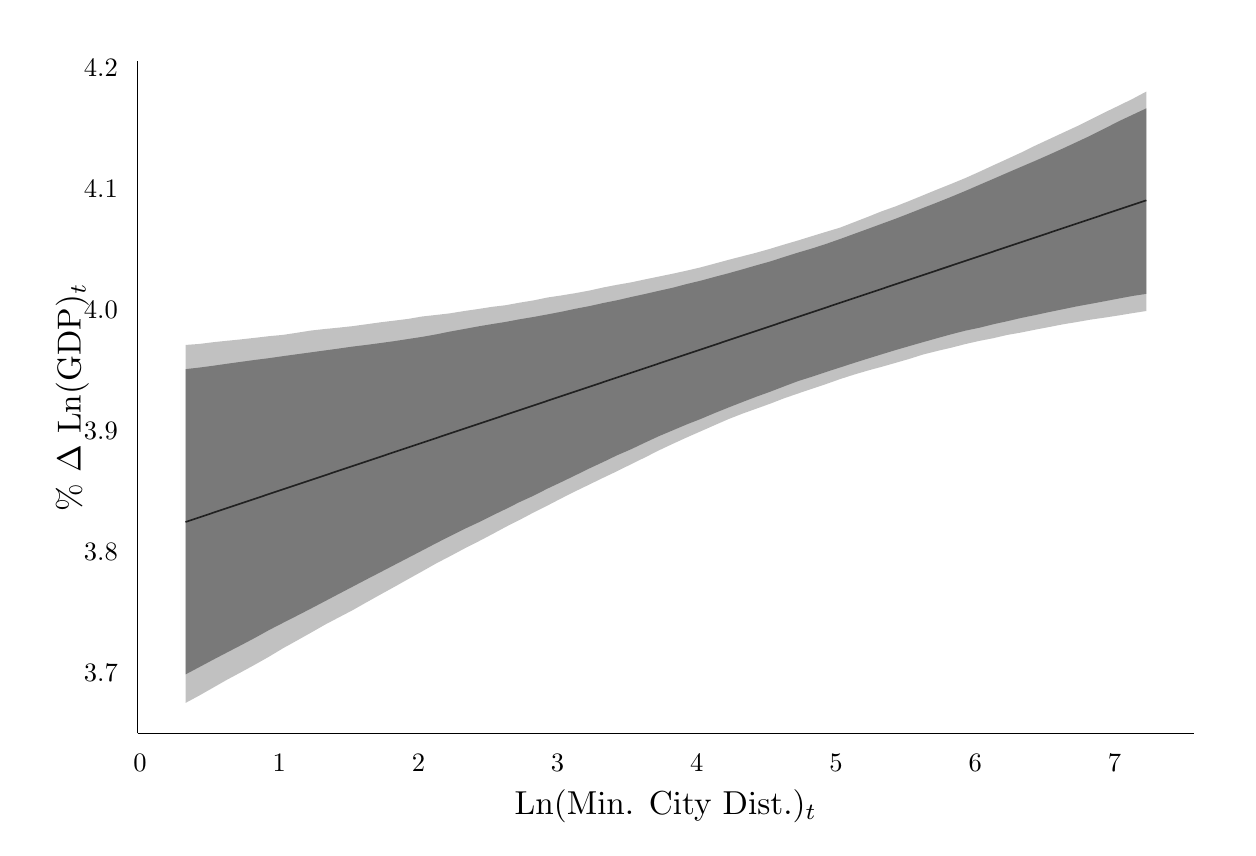
\begin{tikzpicture}[x=1pt,y=1pt]
\definecolor[named]{fillColor}{rgb}{1.00,1.00,1.00}
\path[use as bounding box,fill=fillColor,fill opacity=0.00] (0,0) rectangle (433.62,289.08);
\begin{scope}
\path[clip] (  0.00,  0.00) rectangle (433.62,289.08);
\definecolor[named]{drawColor}{rgb}{1.00,1.00,1.00}
\definecolor[named]{fillColor}{rgb}{1.00,1.00,1.00}

\path[draw=drawColor,line width= 0.6pt,line join=round,line cap=round,fill=fillColor] (  0.00,  0.00) rectangle (433.62,289.08);
\end{scope}
\begin{scope}
\path[clip] ( 39.69, 34.03) rectangle (421.57,277.03);
\definecolor[named]{fillColor}{rgb}{1.00,1.00,1.00}

\path[fill=fillColor] ( 39.69, 34.03) rectangle (421.57,277.03);
\definecolor[named]{drawColor}{rgb}{0.00,0.00,0.00}

\path[draw=drawColor,line width= 0.6pt,line join=round] ( 57.05,110.46) --
	( 62.08,112.14) --
	( 67.11,113.83) --
	( 72.14,115.51) --
	( 77.17,117.20) --
	( 82.20,118.88) --
	( 87.23,120.57) --
	( 92.27,122.25) --
	( 97.30,123.94) --
	(102.33,125.62) --
	(107.36,127.30) --
	(112.39,128.99) --
	(117.42,130.67) --
	(122.45,132.36) --
	(127.49,134.04) --
	(132.52,135.73) --
	(137.55,137.41) --
	(142.58,139.10) --
	(147.61,140.78) --
	(152.64,142.47) --
	(157.67,144.15) --
	(162.71,145.84) --
	(167.74,147.52) --
	(172.77,149.20) --
	(177.80,150.89) --
	(182.83,152.57) --
	(187.86,154.26) --
	(192.89,155.94) --
	(197.93,157.63) --
	(202.96,159.31) --
	(207.99,161.00) --
	(213.02,162.68) --
	(218.05,164.37) --
	(223.08,166.05) --
	(228.12,167.74) --
	(233.15,169.42) --
	(238.18,171.11) --
	(243.21,172.79) --
	(248.24,174.47) --
	(253.27,176.16) --
	(258.30,177.84) --
	(263.34,179.53) --
	(268.37,181.21) --
	(273.40,182.90) --
	(278.43,184.58) --
	(283.46,186.27) --
	(288.49,187.95) --
	(293.52,189.64) --
	(298.56,191.32) --
	(303.59,193.01) --
	(308.62,194.69) --
	(313.65,196.38) --
	(318.68,198.06) --
	(323.71,199.74) --
	(328.74,201.43) --
	(333.78,203.11) --
	(338.81,204.80) --
	(343.84,206.48) --
	(348.87,208.17) --
	(353.90,209.85) --
	(358.93,211.54) --
	(363.96,213.22) --
	(369.00,214.91) --
	(374.03,216.59) --
	(379.06,218.28) --
	(384.09,219.96) --
	(389.12,221.65) --
	(394.15,223.33) --
	(399.18,225.01) --
	(404.22,226.70);
\definecolor[named]{fillColor}{rgb}{0.20,0.20,0.20}

\path[fill=fillColor,fill opacity=0.30] ( 57.05,174.43) --
	( 62.08,174.80) --
	( 67.11,175.43) --
	( 72.14,175.95) --
	( 77.17,176.45) --
	( 82.20,177.01) --
	( 87.23,177.60) --
	( 92.27,178.07) --
	( 97.30,178.83) --
	(102.33,179.63) --
	(107.36,180.19) --
	(112.39,180.68) --
	(117.42,181.22) --
	(122.45,181.91) --
	(127.49,182.61) --
	(132.52,183.22) --
	(137.55,183.85) --
	(142.58,184.72) --
	(147.61,185.27) --
	(152.64,185.85) --
	(157.67,186.68) --
	(162.71,187.40) --
	(167.74,188.19) --
	(172.77,188.79) --
	(177.80,189.72) --
	(182.83,190.53) --
	(187.86,191.58) --
	(192.89,192.32) --
	(197.93,193.15) --
	(202.96,194.08) --
	(207.99,195.20) --
	(213.02,196.17) --
	(218.05,197.04) --
	(223.08,198.12) --
	(228.12,199.15) --
	(233.15,200.19) --
	(238.18,201.29) --
	(243.21,202.47) --
	(248.24,203.82) --
	(253.27,205.19) --
	(258.30,206.48) --
	(263.34,207.77) --
	(268.37,209.20) --
	(273.40,210.73) --
	(278.43,212.20) --
	(283.46,213.76) --
	(288.49,215.30) --
	(293.52,216.81) --
	(298.56,218.76) --
	(303.59,220.71) --
	(308.62,222.73) --
	(313.65,224.51) --
	(318.68,226.51) --
	(323.71,228.57) --
	(328.74,230.64) --
	(333.78,232.65) --
	(338.81,234.73) --
	(343.84,236.98) --
	(348.87,239.31) --
	(353.90,241.60) --
	(358.93,243.92) --
	(363.96,246.40) --
	(369.00,248.74) --
	(374.03,251.08) --
	(379.06,253.40) --
	(384.09,255.89) --
	(389.12,258.42) --
	(394.15,260.84) --
	(399.18,263.30) --
	(404.22,265.99) --
	(404.22,186.70) --
	(399.18,185.91) --
	(394.15,185.08) --
	(389.12,184.30) --
	(384.09,183.58) --
	(379.06,182.70) --
	(374.03,181.87) --
	(369.00,180.89) --
	(363.96,179.93) --
	(358.93,178.91) --
	(353.90,178.04) --
	(348.87,176.86) --
	(343.84,175.89) --
	(338.81,174.74) --
	(333.78,173.45) --
	(328.74,172.28) --
	(323.71,171.02) --
	(318.68,169.43) --
	(313.65,167.97) --
	(308.62,166.54) --
	(303.59,165.18) --
	(298.56,163.70) --
	(293.52,162.08) --
	(288.49,160.29) --
	(283.46,158.60) --
	(278.43,156.91) --
	(273.40,155.18) --
	(268.37,153.23) --
	(263.34,151.42) --
	(258.30,149.61) --
	(253.27,147.65) --
	(248.24,145.45) --
	(243.21,143.23) --
	(238.18,141.02) --
	(233.15,138.72) --
	(228.12,136.35) --
	(223.08,133.80) --
	(218.05,131.34) --
	(213.02,128.83) --
	(207.99,126.45) --
	(202.96,124.00) --
	(197.93,121.57) --
	(192.89,119.03) --
	(187.86,116.41) --
	(182.83,113.90) --
	(177.80,111.23) --
	(172.77,108.70) --
	(167.74,105.98) --
	(162.71,103.34) --
	(157.67,100.79) --
	(152.64, 98.10) --
	(147.61, 95.49) --
	(142.58, 92.64) --
	(137.55, 89.85) --
	(132.52, 87.02) --
	(127.49, 84.25) --
	(122.45, 81.44) --
	(117.42, 78.59) --
	(112.39, 75.96) --
	(107.36, 73.32) --
	(102.33, 70.44) --
	( 97.30, 67.62) --
	( 92.27, 64.83) --
	( 87.23, 61.80) --
	( 82.20, 58.96) --
	( 77.17, 56.21) --
	( 72.14, 53.52) --
	( 67.11, 50.65) --
	( 62.08, 47.79) --
	( 57.05, 45.08) --
	cycle;
\definecolor[named]{fillColor}{rgb}{0.20,0.20,0.20}

\path[fill=fillColor,fill opacity=0.50] ( 57.05,165.69) --
	( 62.08,166.26) --
	( 67.11,166.92) --
	( 72.14,167.65) --
	( 77.17,168.34) --
	( 82.20,169.03) --
	( 87.23,169.66) --
	( 92.27,170.38) --
	( 97.30,171.07) --
	(102.33,171.75) --
	(107.36,172.44) --
	(112.39,173.12) --
	(117.42,173.84) --
	(122.45,174.45) --
	(127.49,175.12) --
	(132.52,175.81) --
	(137.55,176.59) --
	(142.58,177.35) --
	(147.61,178.25) --
	(152.64,179.27) --
	(157.67,180.18) --
	(162.71,181.11) --
	(167.74,181.96) --
	(172.77,182.76) --
	(177.80,183.71) --
	(182.83,184.54) --
	(187.86,185.47) --
	(192.89,186.43) --
	(197.93,187.51) --
	(202.96,188.46) --
	(207.99,189.58) --
	(213.02,190.58) --
	(218.05,191.75) --
	(223.08,192.84) --
	(228.12,194.00) --
	(233.15,195.12) --
	(238.18,196.45) --
	(243.21,197.65) --
	(248.24,199.02) --
	(253.27,200.34) --
	(258.30,201.75) --
	(263.34,203.21) --
	(268.37,204.61) --
	(273.40,206.24) --
	(278.43,207.82) --
	(283.46,209.30) --
	(288.49,210.93) --
	(293.52,212.69) --
	(298.56,214.53) --
	(303.59,216.36) --
	(308.62,218.21) --
	(313.65,220.05) --
	(318.68,222.00) --
	(323.71,224.00) --
	(328.74,225.95) --
	(333.78,227.98) --
	(338.81,230.07) --
	(343.84,232.25) --
	(348.87,234.41) --
	(353.90,236.60) --
	(358.93,238.76) --
	(363.96,240.91) --
	(369.00,243.13) --
	(374.03,245.40) --
	(379.06,247.74) --
	(384.09,250.09) --
	(389.12,252.61) --
	(394.15,255.21) --
	(399.18,257.56) --
	(404.22,259.93) --
	(404.22,192.89) --
	(399.18,192.12) --
	(394.15,191.18) --
	(389.12,190.22) --
	(384.09,189.28) --
	(379.06,188.36) --
	(374.03,187.32) --
	(369.00,186.30) --
	(363.96,185.20) --
	(358.93,184.18) --
	(353.90,182.99) --
	(348.87,181.90) --
	(343.84,180.64) --
	(338.81,179.59) --
	(333.78,178.30) --
	(328.74,176.91) --
	(323.71,175.49) --
	(318.68,174.05) --
	(313.65,172.59) --
	(308.62,171.06) --
	(303.59,169.50) --
	(298.56,167.92) --
	(293.52,166.28) --
	(288.49,164.66) --
	(283.46,162.97) --
	(278.43,161.38) --
	(273.40,159.49) --
	(268.37,157.55) --
	(263.34,155.74) --
	(258.30,153.81) --
	(253.27,151.84) --
	(248.24,149.82) --
	(243.21,147.69) --
	(238.18,145.73) --
	(233.15,143.60) --
	(228.12,141.48) --
	(223.08,139.15) --
	(218.05,136.75) --
	(213.02,134.58) --
	(207.99,132.15) --
	(202.96,129.81) --
	(197.93,127.34) --
	(192.89,124.90) --
	(187.86,122.54) --
	(182.83,119.97) --
	(177.80,117.68) --
	(172.77,115.15) --
	(167.74,112.73) --
	(162.71,110.22) --
	(157.67,107.87) --
	(152.64,105.34) --
	(147.61,102.80) --
	(142.58,100.16) --
	(137.55, 97.55) --
	(132.52, 94.94) --
	(127.49, 92.32) --
	(122.45, 89.72) --
	(117.42, 87.08) --
	(112.39, 84.45) --
	(107.36, 81.80) --
	(102.33, 79.16) --
	( 97.30, 76.57) --
	( 92.27, 74.01) --
	( 87.23, 71.42) --
	( 82.20, 68.63) --
	( 77.17, 65.97) --
	( 72.14, 63.37) --
	( 67.11, 60.74) --
	( 62.08, 58.05) --
	( 57.05, 55.38) --
	cycle;
\end{scope}
\begin{scope}
\path[clip] (  0.00,  0.00) rectangle (433.62,289.08);
\definecolor[named]{drawColor}{rgb}{0.00,0.00,0.00}

\path[draw=drawColor,line width= 0.6pt,line join=round] ( 39.69, 34.03) --
	( 39.69,277.03);
\end{scope}
\begin{scope}
\path[clip] (  0.00,  0.00) rectangle (433.62,289.08);
\definecolor[named]{drawColor}{rgb}{0.00,0.00,0.00}

\node[text=drawColor,anchor=base east,inner sep=0pt, outer sep=0pt, scale=  0.96] at ( 32.57, 52.86) {3.7};

\node[text=drawColor,anchor=base east,inner sep=0pt, outer sep=0pt, scale=  0.96] at ( 32.57, 96.58) {3.8};

\node[text=drawColor,anchor=base east,inner sep=0pt, outer sep=0pt, scale=  0.96] at ( 32.57,140.30) {3.9};

\node[text=drawColor,anchor=base east,inner sep=0pt, outer sep=0pt, scale=  0.96] at ( 32.57,184.02) {4.0};

\node[text=drawColor,anchor=base east,inner sep=0pt, outer sep=0pt, scale=  0.96] at ( 32.57,227.74) {4.1};

\node[text=drawColor,anchor=base east,inner sep=0pt, outer sep=0pt, scale=  0.96] at ( 32.57,271.45) {4.2};
\end{scope}
\begin{scope}
\path[clip] (  0.00,  0.00) rectangle (433.62,289.08);
\definecolor[named]{drawColor}{rgb}{0.00,0.00,0.00}

\path[draw=drawColor,line width= 0.6pt,line join=round] ( 39.69, 34.03) --
	(421.57, 34.03);
\end{scope}
\begin{scope}
\path[clip] (  0.00,  0.00) rectangle (433.62,289.08);
\definecolor[named]{drawColor}{rgb}{0.00,0.00,0.00}

\node[text=drawColor,anchor=base,inner sep=0pt, outer sep=0pt, scale=  0.96] at ( 40.56, 20.31) {0};

\node[text=drawColor,anchor=base,inner sep=0pt, outer sep=0pt, scale=  0.96] at ( 90.87, 20.31) {1};

\node[text=drawColor,anchor=base,inner sep=0pt, outer sep=0pt, scale=  0.96] at (141.19, 20.31) {2};

\node[text=drawColor,anchor=base,inner sep=0pt, outer sep=0pt, scale=  0.96] at (191.50, 20.31) {3};

\node[text=drawColor,anchor=base,inner sep=0pt, outer sep=0pt, scale=  0.96] at (241.82, 20.31) {4};

\node[text=drawColor,anchor=base,inner sep=0pt, outer sep=0pt, scale=  0.96] at (292.13, 20.31) {5};

\node[text=drawColor,anchor=base,inner sep=0pt, outer sep=0pt, scale=  0.96] at (342.45, 20.31) {6};

\node[text=drawColor,anchor=base,inner sep=0pt, outer sep=0pt, scale=  0.96] at (392.76, 20.31) {7};
\end{scope}
\begin{scope}
\path[clip] (  0.00,  0.00) rectangle (433.62,289.08);
\definecolor[named]{drawColor}{rgb}{0.00,0.00,0.00}

\node[text=drawColor,anchor=base,inner sep=0pt, outer sep=0pt, scale=  1.20] at (230.63,  4.82) {Ln(Min. City Dist.)$_{t}$};
\end{scope}
\begin{scope}
\path[clip] (  0.00,  0.00) rectangle (433.62,289.08);
\definecolor[named]{drawColor}{rgb}{0.00,0.00,0.00}

\node[text=drawColor,rotate= 90.00,anchor=base,inner sep=0pt, outer sep=0pt, scale=  1.20] at ( 19.11,155.53) {\% $\Delta$ Ln(GDP)$_{t}$};
\end{scope}
\end{tikzpicture}
}
		\label{fig:cityCoef}}
	\end{tabular}
	\caption{Expected values for GDP growth based on scenarios where all variables are held to their constants but Ln(Min. Conflict Dist.) varies from its minimum to maximum. The 90\% interval of each distribution is shaded in dark grey and the 95\% in a lighter color.}
	\label{fig:simsPlot}
\end{figure}

Here we can clearly see that conflicts located farther away from major cities have almost no adverse impact on economic growth. On average, countries for which conflicts are farther away see almost no declines in economic growth and, in fact, are likely to still see positive growth. Where we see more variation, however, is on the effect of conflicts near to major cities. Although on average our model estimates that these more proximate conflicts are associated with negative levels of economic growth our estimate of this effect is highly uncertain. This just indicates to us that more work needs to be done in parsing out possible variation in economic growth levels for those countries that are experiencing conflicts proximate to their major cities. Nonetheless, overall our results are quite in line with our theoretical expectations.

\subsection{Model Performance}

To assess the accuracy and performance of these estimates we employ a simple two-fold cross validation procedure. We use this procedure both to determine the robustness of our coefficient estimates when estimated on different subsamples of our dataset, and to assess how well the results of our model would generalize to an independent dataset. To begin the cross-validation, we split the 653 sanction cases in our dataset into six approximately equal subsets. We then run each model shown in Table \ref{tab:regResults} six times, where in each iteration we left out one subsample to use as a test set. This allows us to compare the prediction accuracy of each model, thereby helping us to determine the gains from incorporating the reciprocity covariates that are key to our argument.

\begin{figure}
	\centering
	\resizebox{.8\textwidth}{!}{% Created by tikzDevice version 0.7.0 on 2014-09-25 14:01:12
% !TEX encoding = UTF-8 Unicode
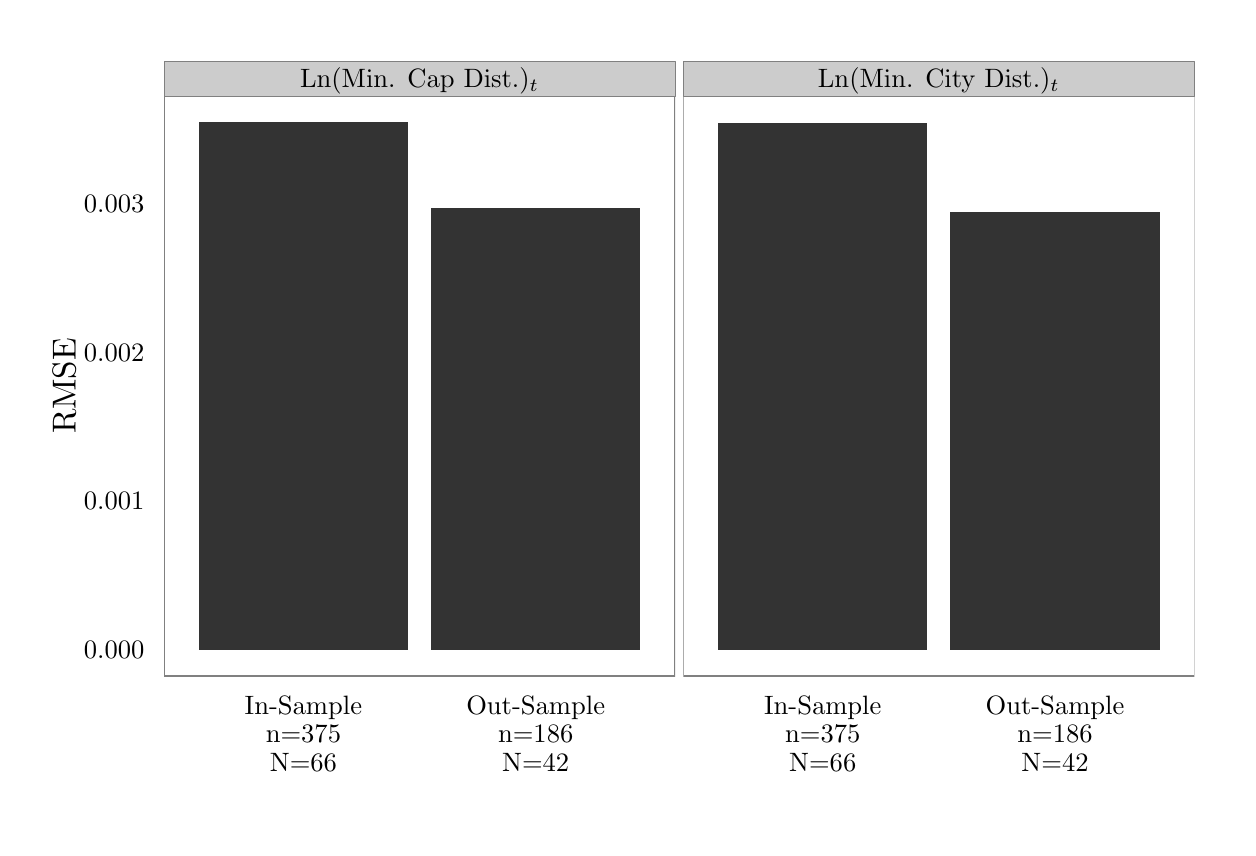
\begin{tikzpicture}[x=1pt,y=1pt]
\definecolor[named]{fillColor}{rgb}{1.00,1.00,1.00}
\path[use as bounding box,fill=fillColor,fill opacity=0.00] (0,0) rectangle (433.62,289.08);
\begin{scope}
\path[clip] (  0.00,  0.00) rectangle (433.62,289.08);
\definecolor[named]{drawColor}{rgb}{1.00,1.00,1.00}
\definecolor[named]{fillColor}{rgb}{1.00,1.00,1.00}

\path[draw=drawColor,line width= 0.6pt,line join=round,line cap=round,fill=fillColor] ( -0.00,  0.00) rectangle (433.62,289.08);
\end{scope}
\begin{scope}
\path[clip] ( 49.28, 54.77) rectangle (233.92,264.40);
\definecolor[named]{fillColor}{rgb}{1.00,1.00,1.00}

\path[fill=fillColor] ( 49.28, 54.77) rectangle (233.92,264.40);
\definecolor[named]{fillColor}{rgb}{0.20,0.20,0.20}

\path[fill=fillColor] ( 61.87, 64.30) rectangle (137.41,254.87);

\path[fill=fillColor] (145.80, 64.30) rectangle (221.33,223.96);
\definecolor[named]{drawColor}{rgb}{0.50,0.50,0.50}

\path[draw=drawColor,line width= 0.6pt,line join=round,line cap=round] ( 49.28, 54.77) rectangle (233.92,264.40);
\end{scope}
\begin{scope}
\path[clip] (236.94, 54.77) rectangle (421.58,264.40);
\definecolor[named]{fillColor}{rgb}{1.00,1.00,1.00}

\path[fill=fillColor] (236.94, 54.77) rectangle (421.58,264.40);
\definecolor[named]{fillColor}{rgb}{0.20,0.20,0.20}

\path[fill=fillColor] (249.52, 64.30) rectangle (325.06,254.81);

\path[fill=fillColor] (333.45, 64.30) rectangle (408.99,222.46);
\definecolor[named]{drawColor}{rgb}{0.50,0.50,0.50}

\path[draw=drawColor,line width= 0.6pt,line join=round,line cap=round] (236.94, 54.77) rectangle (421.58,264.40);
\end{scope}
\begin{scope}
\path[clip] (  0.00,  0.00) rectangle (433.62,289.08);
\definecolor[named]{drawColor}{rgb}{0.50,0.50,0.50}
\definecolor[named]{fillColor}{rgb}{0.80,0.80,0.80}

\path[draw=drawColor,line width= 0.2pt,line join=round,line cap=round,fill=fillColor] ( 49.28,264.40) rectangle (233.92,277.04);
\definecolor[named]{drawColor}{rgb}{0.00,0.00,0.00}

\node[text=drawColor,anchor=base,inner sep=0pt, outer sep=0pt, scale=  0.96] at (141.60,267.41) {Ln(Min. Cap Dist.)$_{t}$};
\end{scope}
\begin{scope}
\path[clip] (  0.00,  0.00) rectangle (433.62,289.08);
\definecolor[named]{drawColor}{rgb}{0.50,0.50,0.50}
\definecolor[named]{fillColor}{rgb}{0.80,0.80,0.80}

\path[draw=drawColor,line width= 0.2pt,line join=round,line cap=round,fill=fillColor] (236.94,264.40) rectangle (421.58,277.04);
\definecolor[named]{drawColor}{rgb}{0.00,0.00,0.00}

\node[text=drawColor,anchor=base,inner sep=0pt, outer sep=0pt, scale=  0.96] at (329.26,267.41) {Ln(Min. City Dist.)$_{t}$};
\end{scope}
\begin{scope}
\path[clip] (  0.00,  0.00) rectangle (433.62,289.08);
\definecolor[named]{drawColor}{rgb}{0.00,0.00,0.00}

\node[text=drawColor,anchor=base east,inner sep=0pt, outer sep=0pt, scale=  0.96] at ( 42.17, 60.99) {0.000};

\node[text=drawColor,anchor=base east,inner sep=0pt, outer sep=0pt, scale=  0.96] at ( 42.17,114.81) {0.001};

\node[text=drawColor,anchor=base east,inner sep=0pt, outer sep=0pt, scale=  0.96] at ( 42.17,168.63) {0.002};

\node[text=drawColor,anchor=base east,inner sep=0pt, outer sep=0pt, scale=  0.96] at ( 42.17,222.44) {0.003};
\end{scope}
\begin{scope}
\path[clip] (  0.00,  0.00) rectangle (433.62,289.08);
\definecolor[named]{drawColor}{rgb}{0.00,0.00,0.00}

\node[text=drawColor,anchor=base,inner sep=0pt, outer sep=0pt, scale=  0.96] at ( 99.64, 41.05) {In-Sample };

\node[text=drawColor,anchor=base,inner sep=0pt, outer sep=0pt, scale=  0.96] at ( 99.64, 30.68) { n=375 };

\node[text=drawColor,anchor=base,inner sep=0pt, outer sep=0pt, scale=  0.96] at ( 99.64, 20.31) { N=66};

\node[text=drawColor,anchor=base,inner sep=0pt, outer sep=0pt, scale=  0.96] at (183.57, 41.05) {Out-Sample };

\node[text=drawColor,anchor=base,inner sep=0pt, outer sep=0pt, scale=  0.96] at (183.57, 30.68) { n=186 };

\node[text=drawColor,anchor=base,inner sep=0pt, outer sep=0pt, scale=  0.96] at (183.57, 20.31) { N=42};
\end{scope}
\begin{scope}
\path[clip] (  0.00,  0.00) rectangle (433.62,289.08);
\definecolor[named]{drawColor}{rgb}{0.00,0.00,0.00}

\node[text=drawColor,anchor=base,inner sep=0pt, outer sep=0pt, scale=  0.96] at (287.29, 41.05) {In-Sample };

\node[text=drawColor,anchor=base,inner sep=0pt, outer sep=0pt, scale=  0.96] at (287.29, 30.68) { n=375 };

\node[text=drawColor,anchor=base,inner sep=0pt, outer sep=0pt, scale=  0.96] at (287.29, 20.31) { N=66};

\node[text=drawColor,anchor=base,inner sep=0pt, outer sep=0pt, scale=  0.96] at (371.22, 41.05) {Out-Sample };

\node[text=drawColor,anchor=base,inner sep=0pt, outer sep=0pt, scale=  0.96] at (371.22, 30.68) { n=186 };

\node[text=drawColor,anchor=base,inner sep=0pt, outer sep=0pt, scale=  0.96] at (371.22, 20.31) { N=42};
\end{scope}
\begin{scope}
\path[clip] (  0.00,  0.00) rectangle (433.62,289.08);
\definecolor[named]{drawColor}{rgb}{0.00,0.00,0.00}

\node[text=drawColor,rotate= 90.00,anchor=base,inner sep=0pt, outer sep=0pt, scale=  1.20] at ( 17.30,159.59) {RMSE};
\end{scope}
\end{tikzpicture}
}
	\caption{In and out of sample performance.}
	\label{fig:rmsePlot}
\end{figure}

First, however, we show the results for our reciprocity covariates when we rerun our survival analysis on each of the six folds from the cross-validation. This analysis helps us to understand whether some of the subsets in our dataset follow a different pattern than what is in the broader set.\footnote{\cite{beck2008time}} Figure \ref{fig:crossval} shows that this is not the case for the analysis we present here, the coefficient estimates for compliance and sanction reciprocity remain consistent across each of these subsamples.\footnote{The parameter estimates for the other covariates also remain consistent across each of the six folds but we leave them out here due to space constraints.}

\begin{figure}
	\centering
	\resizebox{.8\textwidth}{!}{% Created by tikzDevice version 0.7.0 on 2014-09-25 14:00:56
% !TEX encoding = UTF-8 Unicode
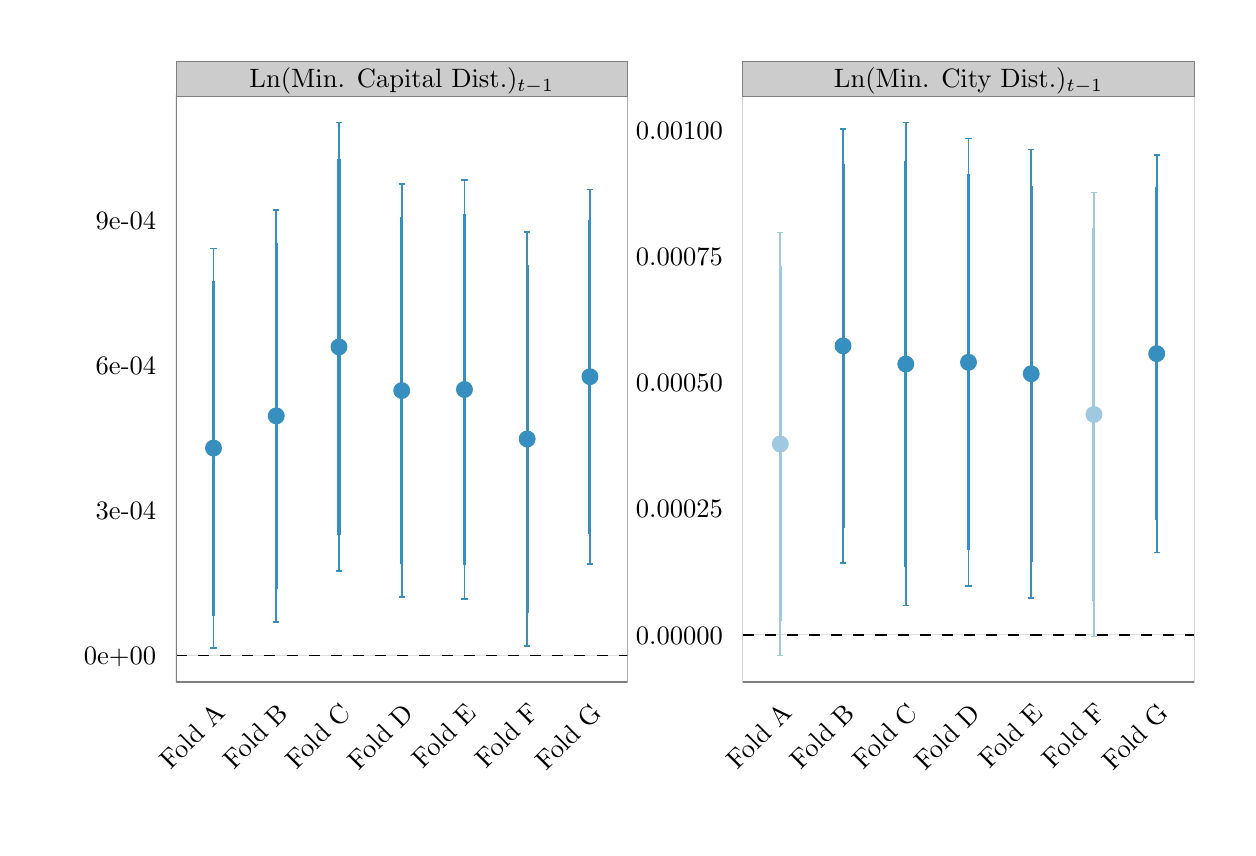
\begin{tikzpicture}[x=1pt,y=1pt]
\definecolor[named]{fillColor}{rgb}{1.00,1.00,1.00}
\path[use as bounding box,fill=fillColor,fill opacity=0.00] (0,0) rectangle (433.62,289.08);
\begin{scope}
\path[clip] (  0.00,  0.00) rectangle (433.62,289.08);
\definecolor[named]{drawColor}{rgb}{1.00,1.00,1.00}
\definecolor[named]{fillColor}{rgb}{1.00,1.00,1.00}

\path[draw=drawColor,line width= 0.6pt,line join=round,line cap=round,fill=fillColor] ( -0.00,  0.00) rectangle (433.62,289.08);
\end{scope}
\begin{scope}
\path[clip] ( 53.55, 52.60) rectangle (216.77,264.40);
\definecolor[named]{fillColor}{rgb}{1.00,1.00,1.00}

\path[fill=fillColor] ( 53.55, 52.60) rectangle (216.77,264.40);
\definecolor[named]{drawColor}{rgb}{0.21,0.56,0.75}
\definecolor[named]{fillColor}{rgb}{0.21,0.56,0.75}

\path[draw=drawColor,draw opacity=0.30,line width= 0.3pt,line join=round,fill=fillColor,fill opacity=0.30] ( 67.15, 65.03) -- ( 67.15,209.31);

\path[draw=drawColor,draw opacity=0.30,line width= 0.3pt,line join=round,fill=fillColor,fill opacity=0.30] ( 89.82, 74.37) -- ( 89.82,223.23);

\path[draw=drawColor,draw opacity=0.30,line width= 0.3pt,line join=round,fill=fillColor,fill opacity=0.30] (112.49, 92.67) -- (112.49,254.77);

\path[draw=drawColor,draw opacity=0.30,line width= 0.3pt,line join=round,fill=fillColor,fill opacity=0.30] (135.16, 83.37) -- (135.16,232.52);

\path[draw=drawColor,draw opacity=0.30,line width= 0.3pt,line join=round,fill=fillColor,fill opacity=0.30] (157.83, 82.70) -- (157.83,233.97);

\path[draw=drawColor,draw opacity=0.30,line width= 0.3pt,line join=round,fill=fillColor,fill opacity=0.30] (180.50, 65.59) -- (180.50,215.32);

\path[draw=drawColor,draw opacity=0.30,line width= 0.3pt,line join=round,fill=fillColor,fill opacity=0.30] (203.17, 95.32) -- (203.17,230.62);
\definecolor[named]{drawColor}{rgb}{0.21,0.56,0.75}
\definecolor[named]{fillColor}{rgb}{0.21,0.56,0.75}

\path[draw=drawColor,line width= 1.1pt,line join=round,fill=fillColor] ( 67.15, 76.63) -- ( 67.15,197.71);

\path[draw=drawColor,line width= 1.1pt,line join=round,fill=fillColor] ( 89.82, 86.34) -- ( 89.82,211.26);

\path[draw=drawColor,line width= 1.1pt,line join=round,fill=fillColor] (112.49,105.70) -- (112.49,241.74);

\path[draw=drawColor,line width= 1.1pt,line join=round,fill=fillColor] (135.16, 95.36) -- (135.16,220.53);

\path[draw=drawColor,line width= 1.1pt,line join=round,fill=fillColor] (157.83, 94.86) -- (157.83,221.81);

\path[draw=drawColor,line width= 1.1pt,line join=round,fill=fillColor] (180.50, 77.62) -- (180.50,203.28);

\path[draw=drawColor,line width= 1.1pt,line join=round,fill=fillColor] (203.17,106.20) -- (203.17,219.75);
\definecolor[named]{drawColor}{rgb}{0.00,0.00,0.00}
\definecolor[named]{fillColor}{rgb}{0.00,0.00,0.00}

\path[draw=drawColor,line width= 0.6pt,dash pattern=on 4pt off 4pt ,line join=round,fill=fillColor] ( 53.55, 62.23) -- (216.77, 62.23);
\definecolor[named]{drawColor}{rgb}{0.21,0.56,0.75}
\definecolor[named]{fillColor}{rgb}{0.21,0.56,0.75}

\path[draw=drawColor,line width= 0.4pt,line join=round,line cap=round,fill=fillColor] ( 67.15,137.17) circle (  2.85);

\path[draw=drawColor,line width= 0.4pt,line join=round,line cap=round,fill=fillColor] ( 89.82,148.80) circle (  2.85);

\path[draw=drawColor,line width= 0.4pt,line join=round,line cap=round,fill=fillColor] (112.49,173.72) circle (  2.85);

\path[draw=drawColor,line width= 0.4pt,line join=round,line cap=round,fill=fillColor] (135.16,157.94) circle (  2.85);

\path[draw=drawColor,line width= 0.4pt,line join=round,line cap=round,fill=fillColor] (157.83,158.33) circle (  2.85);

\path[draw=drawColor,line width= 0.4pt,line join=round,line cap=round,fill=fillColor] (180.50,140.45) circle (  2.85);

\path[draw=drawColor,line width= 0.4pt,line join=round,line cap=round,fill=fillColor] (203.17,162.97) circle (  2.85);

\path[draw=drawColor,line width= 0.6pt,line join=round] ( 66.02,209.31) --
	( 68.29,209.31);

\path[draw=drawColor,line width= 0.6pt,line join=round] ( 67.15,209.31) --
	( 67.15, 65.03);

\path[draw=drawColor,line width= 0.6pt,line join=round] ( 66.02, 65.03) --
	( 68.29, 65.03);

\path[draw=drawColor,line width= 0.6pt,line join=round] ( 88.69,223.23) --
	( 90.95,223.23);

\path[draw=drawColor,line width= 0.6pt,line join=round] ( 89.82,223.23) --
	( 89.82, 74.37);

\path[draw=drawColor,line width= 0.6pt,line join=round] ( 88.69, 74.37) --
	( 90.95, 74.37);

\path[draw=drawColor,line width= 0.6pt,line join=round] (111.36,254.77) --
	(113.62,254.77);

\path[draw=drawColor,line width= 0.6pt,line join=round] (112.49,254.77) --
	(112.49, 92.67);

\path[draw=drawColor,line width= 0.6pt,line join=round] (111.36, 92.67) --
	(113.62, 92.67);

\path[draw=drawColor,line width= 0.6pt,line join=round] (134.03,232.52) --
	(136.29,232.52);

\path[draw=drawColor,line width= 0.6pt,line join=round] (135.16,232.52) --
	(135.16, 83.37);

\path[draw=drawColor,line width= 0.6pt,line join=round] (134.03, 83.37) --
	(136.29, 83.37);

\path[draw=drawColor,line width= 0.6pt,line join=round] (156.70,233.97) --
	(158.96,233.97);

\path[draw=drawColor,line width= 0.6pt,line join=round] (157.83,233.97) --
	(157.83, 82.70);

\path[draw=drawColor,line width= 0.6pt,line join=round] (156.70, 82.70) --
	(158.96, 82.70);

\path[draw=drawColor,line width= 0.6pt,line join=round] (179.37,215.32) --
	(181.63,215.32);

\path[draw=drawColor,line width= 0.6pt,line join=round] (180.50,215.32) --
	(180.50, 65.59);

\path[draw=drawColor,line width= 0.6pt,line join=round] (179.37, 65.59) --
	(181.63, 65.59);

\path[draw=drawColor,line width= 0.6pt,line join=round] (202.04,230.62) --
	(204.30,230.62);

\path[draw=drawColor,line width= 0.6pt,line join=round] (203.17,230.62) --
	(203.17, 95.32);

\path[draw=drawColor,line width= 0.6pt,line join=round] (202.04, 95.32) --
	(204.30, 95.32);
\definecolor[named]{drawColor}{rgb}{0.50,0.50,0.50}

\path[draw=drawColor,line width= 0.6pt,line join=round,line cap=round] ( 53.55, 52.60) rectangle (216.77,264.40);
\end{scope}
\begin{scope}
\path[clip] (258.35, 52.60) rectangle (421.58,264.40);
\definecolor[named]{fillColor}{rgb}{1.00,1.00,1.00}

\path[fill=fillColor] (258.35, 52.60) rectangle (421.57,264.40);
\definecolor[named]{drawColor}{rgb}{0.62,0.79,0.88}
\definecolor[named]{fillColor}{rgb}{0.62,0.79,0.88}

\path[draw=drawColor,draw opacity=0.30,line width= 0.3pt,line join=round,fill=fillColor,fill opacity=0.30] (271.96, 62.23) -- (271.96,215.06);
\definecolor[named]{drawColor}{rgb}{0.21,0.56,0.75}
\definecolor[named]{fillColor}{rgb}{0.21,0.56,0.75}

\path[draw=drawColor,draw opacity=0.30,line width= 0.3pt,line join=round,fill=fillColor,fill opacity=0.30] (294.63, 95.75) -- (294.63,252.44);

\path[draw=drawColor,draw opacity=0.30,line width= 0.3pt,line join=round,fill=fillColor,fill opacity=0.30] (317.30, 80.30) -- (317.30,254.77);

\path[draw=drawColor,draw opacity=0.30,line width= 0.3pt,line join=round,fill=fillColor,fill opacity=0.30] (339.96, 87.24) -- (339.96,249.09);

\path[draw=drawColor,draw opacity=0.30,line width= 0.3pt,line join=round,fill=fillColor,fill opacity=0.30] (362.63, 83.04) -- (362.63,245.02);
\definecolor[named]{drawColor}{rgb}{0.62,0.79,0.88}
\definecolor[named]{fillColor}{rgb}{0.62,0.79,0.88}

\path[draw=drawColor,draw opacity=0.30,line width= 0.3pt,line join=round,fill=fillColor,fill opacity=0.30] (385.30, 69.14) -- (385.30,229.47);
\definecolor[named]{drawColor}{rgb}{0.21,0.56,0.75}
\definecolor[named]{fillColor}{rgb}{0.21,0.56,0.75}

\path[draw=drawColor,draw opacity=0.30,line width= 0.3pt,line join=round,fill=fillColor,fill opacity=0.30] (407.97, 99.45) -- (407.97,243.12);
\definecolor[named]{drawColor}{rgb}{0.62,0.79,0.88}
\definecolor[named]{fillColor}{rgb}{0.62,0.79,0.88}

\path[draw=drawColor,line width= 1.1pt,line join=round,fill=fillColor] (271.96, 74.51) -- (271.96,202.78);
\definecolor[named]{drawColor}{rgb}{0.21,0.56,0.75}
\definecolor[named]{fillColor}{rgb}{0.21,0.56,0.75}

\path[draw=drawColor,line width= 1.1pt,line join=round,fill=fillColor] (294.63,108.35) -- (294.63,239.84);

\path[draw=drawColor,line width= 1.1pt,line join=round,fill=fillColor] (317.30, 94.33) -- (317.30,240.75);

\path[draw=drawColor,line width= 1.1pt,line join=round,fill=fillColor] (339.96,100.25) -- (339.96,236.08);

\path[draw=drawColor,line width= 1.1pt,line join=round,fill=fillColor] (362.63, 96.06) -- (362.63,232.00);
\definecolor[named]{drawColor}{rgb}{0.62,0.79,0.88}
\definecolor[named]{fillColor}{rgb}{0.62,0.79,0.88}

\path[draw=drawColor,line width= 1.1pt,line join=round,fill=fillColor] (385.30, 82.03) -- (385.30,216.58);
\definecolor[named]{drawColor}{rgb}{0.21,0.56,0.75}
\definecolor[named]{fillColor}{rgb}{0.21,0.56,0.75}

\path[draw=drawColor,line width= 1.1pt,line join=round,fill=fillColor] (407.97,111.00) -- (407.97,231.57);
\definecolor[named]{drawColor}{rgb}{0.00,0.00,0.00}
\definecolor[named]{fillColor}{rgb}{0.00,0.00,0.00}

\path[draw=drawColor,line width= 0.6pt,dash pattern=on 4pt off 4pt ,line join=round,fill=fillColor] (258.35, 69.66) -- (421.58, 69.66);
\definecolor[named]{drawColor}{rgb}{0.62,0.79,0.88}
\definecolor[named]{fillColor}{rgb}{0.62,0.79,0.88}

\path[draw=drawColor,line width= 0.4pt,line join=round,line cap=round,fill=fillColor] (271.96,138.64) circle (  2.85);
\definecolor[named]{drawColor}{rgb}{0.21,0.56,0.75}
\definecolor[named]{fillColor}{rgb}{0.21,0.56,0.75}

\path[draw=drawColor,line width= 0.4pt,line join=round,line cap=round,fill=fillColor] (294.63,174.10) circle (  2.85);

\path[draw=drawColor,line width= 0.4pt,line join=round,line cap=round,fill=fillColor] (317.30,167.54) circle (  2.85);

\path[draw=drawColor,line width= 0.4pt,line join=round,line cap=round,fill=fillColor] (339.96,168.16) circle (  2.85);

\path[draw=drawColor,line width= 0.4pt,line join=round,line cap=round,fill=fillColor] (362.63,164.03) circle (  2.85);
\definecolor[named]{drawColor}{rgb}{0.62,0.79,0.88}
\definecolor[named]{fillColor}{rgb}{0.62,0.79,0.88}

\path[draw=drawColor,line width= 0.4pt,line join=round,line cap=round,fill=fillColor] (385.30,149.31) circle (  2.85);
\definecolor[named]{drawColor}{rgb}{0.21,0.56,0.75}
\definecolor[named]{fillColor}{rgb}{0.21,0.56,0.75}

\path[draw=drawColor,line width= 0.4pt,line join=round,line cap=round,fill=fillColor] (407.97,171.29) circle (  2.85);
\definecolor[named]{drawColor}{rgb}{0.62,0.79,0.88}

\path[draw=drawColor,line width= 0.6pt,line join=round] (270.82,215.06) --
	(273.09,215.06);

\path[draw=drawColor,line width= 0.6pt,line join=round] (271.96,215.06) --
	(271.96, 62.23);

\path[draw=drawColor,line width= 0.6pt,line join=round] (270.82, 62.23) --
	(273.09, 62.23);
\definecolor[named]{drawColor}{rgb}{0.21,0.56,0.75}

\path[draw=drawColor,line width= 0.6pt,line join=round] (293.49,252.44) --
	(295.76,252.44);

\path[draw=drawColor,line width= 0.6pt,line join=round] (294.63,252.44) --
	(294.63, 95.75);

\path[draw=drawColor,line width= 0.6pt,line join=round] (293.49, 95.75) --
	(295.76, 95.75);

\path[draw=drawColor,line width= 0.6pt,line join=round] (316.16,254.77) --
	(318.43,254.77);

\path[draw=drawColor,line width= 0.6pt,line join=round] (317.30,254.77) --
	(317.30, 80.30);

\path[draw=drawColor,line width= 0.6pt,line join=round] (316.16, 80.30) --
	(318.43, 80.30);

\path[draw=drawColor,line width= 0.6pt,line join=round] (338.83,249.09) --
	(341.10,249.09);

\path[draw=drawColor,line width= 0.6pt,line join=round] (339.96,249.09) --
	(339.96, 87.24);

\path[draw=drawColor,line width= 0.6pt,line join=round] (338.83, 87.24) --
	(341.10, 87.24);

\path[draw=drawColor,line width= 0.6pt,line join=round] (361.50,245.02) --
	(363.77,245.02);

\path[draw=drawColor,line width= 0.6pt,line join=round] (362.63,245.02) --
	(362.63, 83.04);

\path[draw=drawColor,line width= 0.6pt,line join=round] (361.50, 83.04) --
	(363.77, 83.04);
\definecolor[named]{drawColor}{rgb}{0.62,0.79,0.88}

\path[draw=drawColor,line width= 0.6pt,line join=round] (384.17,229.47) --
	(386.44,229.47);

\path[draw=drawColor,line width= 0.6pt,line join=round] (385.30,229.47) --
	(385.30, 69.14);

\path[draw=drawColor,line width= 0.6pt,line join=round] (384.17, 69.14) --
	(386.44, 69.14);
\definecolor[named]{drawColor}{rgb}{0.21,0.56,0.75}

\path[draw=drawColor,line width= 0.6pt,line join=round] (406.84,243.12) --
	(409.11,243.12);

\path[draw=drawColor,line width= 0.6pt,line join=round] (407.97,243.12) --
	(407.97, 99.45);

\path[draw=drawColor,line width= 0.6pt,line join=round] (406.84, 99.45) --
	(409.11, 99.45);
\definecolor[named]{drawColor}{rgb}{0.50,0.50,0.50}

\path[draw=drawColor,line width= 0.6pt,line join=round,line cap=round] (258.35, 52.60) rectangle (421.57,264.40);
\end{scope}
\begin{scope}
\path[clip] (  0.00,  0.00) rectangle (433.62,289.08);
\definecolor[named]{drawColor}{rgb}{0.50,0.50,0.50}
\definecolor[named]{fillColor}{rgb}{0.80,0.80,0.80}

\path[draw=drawColor,line width= 0.2pt,line join=round,line cap=round,fill=fillColor] ( 53.55,264.40) rectangle (216.77,277.04);
\definecolor[named]{drawColor}{rgb}{0.00,0.00,0.00}

\node[text=drawColor,anchor=base,inner sep=0pt, outer sep=0pt, scale=  0.96] at (135.16,267.41) {Ln(Min. Capital Dist.)$_{t-1}$};
\end{scope}
\begin{scope}
\path[clip] (  0.00,  0.00) rectangle (433.62,289.08);
\definecolor[named]{drawColor}{rgb}{0.50,0.50,0.50}
\definecolor[named]{fillColor}{rgb}{0.80,0.80,0.80}

\path[draw=drawColor,line width= 0.2pt,line join=round,line cap=round,fill=fillColor] (258.35,264.40) rectangle (421.57,277.04);
\definecolor[named]{drawColor}{rgb}{0.00,0.00,0.00}

\node[text=drawColor,anchor=base,inner sep=0pt, outer sep=0pt, scale=  0.96] at (339.96,267.41) {Ln(Min. City Dist.)$_{t-1}$};
\end{scope}
\begin{scope}
\path[clip] (  0.00,  0.00) rectangle (433.62,289.08);
\definecolor[named]{drawColor}{rgb}{0.00,0.00,0.00}

\node[text=drawColor,anchor=base east,inner sep=0pt, outer sep=0pt, scale=  0.96] at ( 46.44, 58.92) {0e+00};

\node[text=drawColor,anchor=base east,inner sep=0pt, outer sep=0pt, scale=  0.96] at ( 46.44,111.38) {3e-04};

\node[text=drawColor,anchor=base east,inner sep=0pt, outer sep=0pt, scale=  0.96] at ( 46.44,163.84) {6e-04};

\node[text=drawColor,anchor=base east,inner sep=0pt, outer sep=0pt, scale=  0.96] at ( 46.44,216.30) {9e-04};
\end{scope}
\begin{scope}
\path[clip] (  0.00,  0.00) rectangle (433.62,289.08);
\definecolor[named]{drawColor}{rgb}{0.00,0.00,0.00}

\node[text=drawColor,anchor=base east,inner sep=0pt, outer sep=0pt, scale=  0.96] at (251.24, 66.35) {0.00000};

\node[text=drawColor,anchor=base east,inner sep=0pt, outer sep=0pt, scale=  0.96] at (251.24,111.91) {0.00025};

\node[text=drawColor,anchor=base east,inner sep=0pt, outer sep=0pt, scale=  0.96] at (251.24,157.46) {0.00050};

\node[text=drawColor,anchor=base east,inner sep=0pt, outer sep=0pt, scale=  0.96] at (251.24,203.02) {0.00075};

\node[text=drawColor,anchor=base east,inner sep=0pt, outer sep=0pt, scale=  0.96] at (251.24,248.58) {0.00100};
\end{scope}
\begin{scope}
\path[clip] (  0.00,  0.00) rectangle (433.62,289.08);
\definecolor[named]{drawColor}{rgb}{0.00,0.00,0.00}

\node[text=drawColor,rotate= 45.00,anchor=base east,inner sep=0pt, outer sep=0pt, scale=  0.96] at ( 71.83, 40.81) {Fold A};

\node[text=drawColor,rotate= 45.00,anchor=base east,inner sep=0pt, outer sep=0pt, scale=  0.96] at ( 94.50, 40.81) {Fold B};

\node[text=drawColor,rotate= 45.00,anchor=base east,inner sep=0pt, outer sep=0pt, scale=  0.96] at (117.17, 40.81) {Fold C};

\node[text=drawColor,rotate= 45.00,anchor=base east,inner sep=0pt, outer sep=0pt, scale=  0.96] at (139.84, 40.81) {Fold D};

\node[text=drawColor,rotate= 45.00,anchor=base east,inner sep=0pt, outer sep=0pt, scale=  0.96] at (162.51, 40.81) {Fold E};

\node[text=drawColor,rotate= 45.00,anchor=base east,inner sep=0pt, outer sep=0pt, scale=  0.96] at (185.17, 40.81) {Fold F};

\node[text=drawColor,rotate= 45.00,anchor=base east,inner sep=0pt, outer sep=0pt, scale=  0.96] at (207.84, 40.81) {Fold G};
\end{scope}
\begin{scope}
\path[clip] (  0.00,  0.00) rectangle (433.62,289.08);
\definecolor[named]{drawColor}{rgb}{0.00,0.00,0.00}

\node[text=drawColor,rotate= 45.00,anchor=base east,inner sep=0pt, outer sep=0pt, scale=  0.96] at (276.63, 40.81) {Fold A};

\node[text=drawColor,rotate= 45.00,anchor=base east,inner sep=0pt, outer sep=0pt, scale=  0.96] at (299.30, 40.81) {Fold B};

\node[text=drawColor,rotate= 45.00,anchor=base east,inner sep=0pt, outer sep=0pt, scale=  0.96] at (321.97, 40.81) {Fold C};

\node[text=drawColor,rotate= 45.00,anchor=base east,inner sep=0pt, outer sep=0pt, scale=  0.96] at (344.64, 40.81) {Fold D};

\node[text=drawColor,rotate= 45.00,anchor=base east,inner sep=0pt, outer sep=0pt, scale=  0.96] at (367.31, 40.81) {Fold E};

\node[text=drawColor,rotate= 45.00,anchor=base east,inner sep=0pt, outer sep=0pt, scale=  0.96] at (389.98, 40.81) {Fold F};

\node[text=drawColor,rotate= 45.00,anchor=base east,inner sep=0pt, outer sep=0pt, scale=  0.96] at (412.65, 40.81) {Fold G};
\end{scope}
\end{tikzpicture}
}
	\caption{Each row here shows the coefficient estimate of distance from rerunning the model on eight random subsamples within the dataset. All the covariates used in the initial models were included as well.}
	\label{fig:crossPlot}
\end{figure}